%===============================================================================
% LaTeX sjabloon voor de bachelorproef toegepaste informatica aan HOGENT
% Meer info op https://github.com/HoGentTIN/bachproef-latex-sjabloon
%===============================================================================

\documentclass[dvipsnames]{bachproef-tin}

\usepackage{hogent-thesis-titlepage} % Titelpagina conform aan HOGENT huisstijl

\usepackage{caption}
\usepackage{xcolor}
\usepackage{biblatex}
\addbibresource{bachproef-tin.bib}


%%---------- Documenteigenschappen ---------------------------------------------

% De titel van het rapport/bachelorproef
\title{Het bepalen van een optimale opstelling voor de registratie van de locatie en de verplaatsing van locatie van een voorwerp binnen een gebouw}

% Je eigen naam
\author{Cedric Delaruelle}

% De naam van je promotor (lector van de opleiding)
\promotor{Johan Van Schoor}

% De naam van je co-promotor. Als je promotor ook je opdrachtgever is en je
% dus ook inhoudelijk begeleidt (en enkel dan!), mag je dit leeg laten.
\copromotor{Pieter Suanet}

% Indien je bachelorproef in opdracht van/in samenwerking met een bedrijf of
% externe organisatie geschreven is, geef je hier de naam. Zoniet laat je dit
% zoals het is.
\instelling{Aucxis}

% Academiejaar
\academiejaar{2021-2022}

% Examenperiode
%  - 1e semester = 1e examenperiode => 1
%  - 2e semester = 2e examenperiode => 2
%  - tweede zit  = 3e examenperiode => 3
\examenperiode{2}

%===============================================================================
% Inhoud document
%===============================================================================

\begin{document}

%---------- Taalselectie -------------------------------------------------------
% Als je je bachelorproef in het Engels schrijft, haal dan onderstaande regel
% uit commentaar. Let op: de tekst op de voorkaft blijft in het Nederlands, en
% dat is ook de bedoeling!

%\selectlanguage{english}

%---------- Titelblad ----------------------------------------------------------
\inserttitlepage

%---------- Samenvatting, voorwoord --------------------------------------------
\usechapterimagefalse
%%=============================================================================
%% Voorwoord
%%=============================================================================

\chapter*{\IfLanguageName{dutch}{Woord vooraf}{Preface}}
\label{ch:voorwoord}

%% TODO:
%% Het voorwoord is het enige deel van de bachelorproef waar je vanuit je
%% eigen standpunt (``ik-vorm'') mag schrijven. Je kan hier bv. motiveren
%% waarom jij het onderwerp wil bespreken.
%% Vergeet ook niet te bedanken wie je geholpen/gesteund/... heeft


%%=============================================================================
%% Samenvatting
%%=============================================================================

% TODO: De "abstract" of samenvatting is een kernachtige (~ 1 blz. voor een
% thesis) synthese van het document.
%
% Deze aspecten moeten zeker aan bod komen:
% - Context: waarom is dit werk belangrijk?
% - Nood: waarom moest dit onderzocht worden?
% - Taak: wat heb je precies gedaan?
% - Object: wat staat in dit document geschreven?
% - Resultaat: wat was het resultaat?
% - Conclusie: wat is/zijn de belangrijkste conclusie(s)?
% - Perspectief: blijven er nog vragen open die in de toekomst nog kunnen
%    onderzocht worden? Wat is een mogelijk vervolg voor jouw onderzoek?
%
% LET OP! Een samenvatting is GEEN voorwoord!

%%---------- Nederlandse samenvatting -----------------------------------------
%
% TODO: Als je je bachelorproef in het Engels schrijft, moet je eerst een
% Nederlandse samenvatting invoegen. Haal daarvoor onderstaande code uit
% commentaar.
% Wie zijn bachelorproef in het Nederlands schrijft, kan dit negeren, de inhoud
% wordt niet in het document ingevoegd.

\IfLanguageName{english}{%
\selectlanguage{dutch}
\chapter*{Samenvatting}
\lipsum[1-4]
\selectlanguage{english}
}{}

%%---------- Samenvatting -----------------------------------------------------
% De samenvatting in de hoofdtaal van het document

\chapter*{\IfLanguageName{dutch}{Samenvatting}{Abstract}}

\lipsum[1-4]


%---------- Inhoudstafel -------------------------------------------------------
\pagestyle{empty} % Geen hoofding
\tableofcontents  % Voeg de inhoudstafel toe
\cleardoublepage  % Zorg dat volgende hoofstuk op een oneven pagina begint
\pagestyle{fancy} % Zet hoofding opnieuw aan

%---------- Lijst figuren, afkortingen, ... ------------------------------------

% Indien gewenst kan je hier een lijst van figuren/tabellen opgeven. Geef in
% dat geval je figuren/tabellen altijd een korte beschrijving:
%
%  \caption[korte beschrijving]{uitgebreide beschrijving}
%
% De korte beschrijving wordt gebruikt voor deze lijst, de uitgebreide staat bij
% de figuur of tabel zelf.

\listoffigures
\listoftables

% Als je een lijst van afkortingen of termen wil toevoegen, dan hoort die
% hier thuis. Gebruik bijvoorbeeld de ``glossaries'' package.
% https://www.overleaf.com/learn/latex/Glossaries

%---------- Kern ---------------------------------------------------------------

% De eerste hoofdstukken van een bachelorproef zijn meestal een inleiding op
% het onderwerp, literatuurstudie en verantwoording methodologie.
% Aarzel niet om een meer beschrijvende titel aan deze hoofstukken te geven of
% om bijvoorbeeld de inleiding en/of stand van zaken over meerdere hoofdstukken
% te verspreiden!

%%=============================================================================
%% Inleiding
%%=============================================================================

\chapter{Inleiding}
\label{ch:inleiding}

\section{Probleemstelling}
\label{sec:probleemstelling}

Momenteel is Aucxis, de opdrachtgever en partner voor dit onderzoek, bezig met het uitwerken en ontwikkelen van hun Polaris platform. Het voornaamste doel van dit platform is het kunnen volgen van voorwerpen binnen en buiten bedrijven. Dit aan de hand van verschillende technologieën, voornamelijk RFID en BLE binnen het bedrijf, en GPS daarbuiten. 
Het concept van dit platform is dat er logische locaties bestaan (zoals warenhuis 1 of keuken), waar de voorwerpen zich bevinden. Voor een goede werking van dit systeem is het duidelijk nodig dat uit de data bekomen uit de hardware kan afgeleid worden op welke logische locatie een voorwerp zich bevind en wanneer het zich verplaatst tussen locaties. Dit is geen normaal softwareprobleem want logischerwijs zal de manier waarop de hardware staat opgesteld een grote invloed hebben op de nauwkeurigheid en correctheid van deze lokalisaties en verplaatsingen. Hierdoor is het van groot belang voor de correcte werking van dit platform dat er een goede opstelling wordt gekozen. Om dit te kunnen doen is er een onderzoek nodig naar wat deze optimale opstelling zou kunnen zijn. Dit is ook de reden dat dit onderzoek in het leven is geroepen.

\section{Wie is Aucxis}
\label{sec:wie-is-aucxis}
Aucxis is een bedrijf gevestigd te Stekene, welke actief is sinds 1983. Bij oprichting was het een bedrijf dat zich toespitste op het ontwikkelen van eenderzijds de bewaring (Procescontrole), en anderzijds de veilinginfrastructuur (E-trade) voor groenten en fruit. Het werd hier vrij snel een toonaangevend bedrijf en werd wereldleider tegen 2000. Later, in 2007 richtten ze een 3e businessunit op, namelijk de RFID divisie, welke zich focust op het onderzoek naar en ontwikkeling van RFID toepassingen. Vandaag is het nog steeds een toonaangevend bedrijf met in-house oplossingen voor allerhande toepassingen binnen deze sectoren en zijn ze nog steeds actief bezig aan de optimalisering en uitbreiding hiervan. Recentelijk zijn ze ook geïnteresseerd geworden in het uitbreiden van hun praktijken naar BLE toepassingen.\autocite{Aucxis2020}

\section{Onderzoeksvraag}
\label{sec:onderzoeksvraag}

Zoals duidelijk is geworden in de probleemstelling is er nood aan een onderzoek voor het vinden van een zo optimaal mogelijke opstelling voor het bepalen van de locatie waar een voorwerp zich bevind. Verder is ook de detectie van een verplaatsing belangrijk, dit gebeurt als de locatie van het voorwerp verandert. Met oog op deze probleemstelling luidt de onderzoeksvraag voor deze bachelorproef als volgt:
\begin{center}
	\textbf{Welke hardwareopstelling, bestaande uit RFID of BLE componenten, is optimaal voor de plaats- en verplaatsingsbepaling van een voorwerp binnen een gebouw.}
\end{center}
Deze vraag omvangt goed de essentie van de situatie die dient onderzocht te worden, namelijk de beste opstelling voor het volgen van een voorwerp binnen een gebouw, en dit met RFID of BLE technologie. Binnen de probleemstelling werd echter ook aangegeven dat binnen de scope van Polaris ook gps lokalisatie voor voorwerpen buiten het bedrijf aanwezig was. Locatiebepaling met behulp van gps is echter al goed ingeburgerd, waardoor er voldoende bronnen zijn en dit ook duidelijk en precies is. Door deze reden is er geen nut om dit ook te onderzoeken en wordt dit onderdeel buiten de scope van dit onderzoek gehouden. Plaatsbepalingen binnen zijn echter niet zo optimaal voor gps aangezien de meeste gebouwen/kantoren beschikken over verdiepen (waar er meerdere locaties dezelfde geografische coördinaat hebben), en gps ook een bepaalde onzekerheid heeft op de meting.

\section{Onderzoeksdoelstelling}
\label{sec:onderzoeksdoelstelling}

Het hoofddoel van dit onderzoek is het vergelijken van een aantal opstellingen, met RFID of met BLE, en met verschillende concepten achter hun werking. De verschillende opstellingen met hun theoretische achtergrond volgen verder in dit verslag. Zoals de onderzoeksvraag echter al doet vermoeden is het doel niet louter een vergelijkende studie, aangezien het ook de bedoeling is dat er een optimale opstelling uit de bus komt. 
In praktijk zal er nooit een opstelling zijn die de beste is, aangezien er altijd een afweging zal zijn tussen de nauwkeurigheid en de kostprijs van de opstelling. Ook zullen sommige opstellingen beter zijn in bepaalde situaties dan andere. Wel zal het mogelijk zijn om totaal onpraktische en onnauwkeurige opstellingen uit te branden. De conclusie zal eerder een afweging geven tussen de verschillende opstellingen, maar zal zeker geen louter vergelijkende aard hebben.

\section{Opzet van dit onderzoek}
\label{sec:opzet-bachelorproef}

De rest van dit onderzoek is als volgt opgebouwd:

In Hoofdstuk~\ref{ch:literatuurstudie} wordt een overzicht gegeven van de theoretische achtergrond die nodig is voor het begrijpen van het onderzoek en de rest van dit onderzoek. Het bevat informatie over de werking van de RFID en BLE technologieën, definities van veelvoorkomende begrippen en diverse andere benodigde uitleg.

In Hoofdstuk~\ref{ch:opstellingen} worden de onderzochte opstellingen opgesomd, samen met een theoretische achtergrond. Het is een projectie van de kennis opgedaan tijdens de literatuurstudie op de te onderzoeken opstellingen.

In Hoofdstuk~\ref{ch:methodologie} wordt de methodologie toegelicht en worden de gebruikte onderzoekstechnieken besproken om een antwoord te kunnen formuleren op de onderzoeksvraag.

In Hoofdstuk~\ref{ch:testen} worden de uitgevoerde tests beschreven, de resultaten verwerkt en geconcludeerd.

In Hoofdstuk~\ref{ch:conclusie}, tenslotte, wordt eerst de voornaamste informatie gebundeld, waarna deze gebruikt wordt om een algemene conclusie te gegeven en een antwoord te formuleren op de onderzoeksvraag. Daarna wordt ook een aanzet gegeven voor toekomstig onderzoek binnen dit domein.
%%=============================================================================
%% Literatuurstudie
%%=============================================================================

\chapter{Literatuurstudie}
\label{ch:literatuurstudie}

Dit hoofdstuk zal een overzicht geven van de theoretische achtergrond van de hardware, protocollen, programma's en andere concepten die gebruikt worden bij het gevoerde onderzoek voor het beantwoorden van bovengenoemde onderzoeksvraag.

\section{Definities}
\label{sec:lit-definities}
Deze sectie zal enkele belangrijke begrippen introduceren die belangrijk zullen zijn bij het verdere lezen van dit hoofdstuk en de rest van het document.

\subsubsection{RSSI}
De RSSI, of voluit Received Signal Strength Indicator, is een maat voor de signaalsterkte die een ontvanger ontvangt van bijhorende zender. Ze wordt typisch gebruikt als het over radio-/elektromagnetische golven gaat.\autocite{Admin2022} Ze wordt uitgedrukt in dBm (Decibel per milliwatt).\autocite{Tseard2016} Het is een zeer kleine en logaritmische maat, de waarden in dit document zullen in de grootteorde -10 dBm liggen.

\subsubsection{IoT}
IoT, of voluit Internet Of Things, is een systeem van samenwerkende devices die met elkaar verbonden zijn via het internet, en zo, zonder menselijke tussenkomst, taken uitvoeren. Elk device is geïdentificeerd door een unieke identifier, of UID. Een device in deze context is alles wat met het internet kan verbonden zijn.\autocite{Gillis2022}

\subsubsection{MQTT}
MQTT, of voluit Message Queuing Telemetry Transport, is een protocol voor het versturen van berichten gemaakt door IoT devices over het internet. Belangrijke voordelen van het protocol zijn dat het licht en efficiënt is, en gemakkelijk schaalbaar naar grote hoeveelheden devices.\autocite{MQTT2022}

\subsubsection{FSPL}
FSPL, of voluit Free Space Path Loss, is het theoretische verlies in signaalsterkte over een bepaalde afstand in open ruimte. Deze kan berekend worden, gegeven de afstand tussen de 2 antennes (d), de frequentie van de EM golf (f), en de gain op de zendende en ontvangende antenne (Gz en Go respectievelijk). Ze wordt berekend via onderstaande formule: 
\[FSPL = 20\log_{10}(d) + 20\log_{10}(f) + 20\log_{10}(\frac{4\pi}{c}) - G_z - G_o \]
\autocite{Pasternack2020}

In deze formule staat \(c\) voor de lichtsnelheid \(\approx3x10^5 \frac{m}{s}\)
\autocite{SOL2022}

\subsubsection{Trilateratie}
Trilateratie is de berekening voor de bepaling van de coördinaten van een punt uit 2 geweten punten, en de afstanden van die punten tot het te berekenen punt. Uit deze berekening blijven 2 punten over, 1 boven en 1 onder de lijn tussen de 2 geweten punten. Hiervan is er steeds 1 mogelijk en 1 onmogelijk, dit onmogelijke punt kan hierdoor logisch uitgebrand worden. De formules voor berekening zijn als volgt:
 \[x = \frac{d_1^2 - d_2^2 + (x_2 - x_1)}{2(x_2 - x_1)} + x_1\]
 \[y = \sqrt{d_1^2 - x^2} \pm y_1\]
 Met \((x,  y)\) de coördinaten van het onbekende punt,  \((x_1, y_1)\) en \((x_2, y_1)\) de coördinaten van de geweten punten en \(d_1\) en \(d_2\) de bekende afstanden.
 \autocite{TRM2022}

\section{Hardware}
\label{sec:lit-hardware}
Deze sectie zal de gebruikte hardwaretechnologieën toelichten, deze zijn RFID en BLE.

\subsection{RFID}
\label{subsec:lit-rfid}
RFID, of voluit Radio Frequency IDentification, is een draadloos communicatie systeem welke gebruik maakt van elektromagnetische golven\footnote{Verder in dit document worden deze afgekort als EM golven}. Een typische RFID opstelling bestaat uit 3 delen, nl. een zender/ontvanger combinatie, ook transceiver genoemd, een antenne, en een transponder, ook wel RFID-tag  genoemd.\autocite{Auxcis2022}\autocite{SICK2022} In essentie werkt dit als volgt: de transmitter laat de antenne een EM veld opwekken. Alle RFID-tags die zich in dit veld bevind zullen dit registreren en zij zullen ook een veld opwekken. Deze zal op zijn beurt terug opgevangen worden door de antenne, waarna dit zal doorgegeven worden aan de receiver.
In essentie zal de transmitter een signaal uitsturen, waarop alle RFID-tags binnen bereik zullen antwoorden, waarna dit antwoord terug zal belanden bij de receiver. De combinatie van de transceiver en de antenne wordt vaak een RFID lezer of reader genoemd, aangezien deze onderdelen steeds samen moeten werken en hardwarematig op 1 locatie zullen staan.\autocite{Amster2021}
Deze transceiver is echter meestal niet gelimiteerd tot slechts 1 aangesloten antenne, afhankelijk van de gebruikte hardware kan deze ook 2 of 4 antennes aankoppelen. De data die de transceiver ontvangt van de RFID-tags kan vervolgens via diverse kanalen verzonden worden naar een computer of server die deze dan verder kan afhandelen.

Alhoewel alle onderdelen in de opstelling in vele verschillende geuren en kleuren beschikbaar zijn, verschilt de functionaliteit bij de antenne en transceiver niet zozeer. De antennes kunnen verschillen in oppervlakte en vorm. Dit heeft invloed op de zone waaruit RFID-tags antwoorden zullen sturen. Een vlakke antenne stuurt voor zich uit en verwacht antwoorden van uit die richting, terwijl een staafvormige rondom zich straalt maar niet naar zijn uiteinden. De vorm van antenne beïnvloed ook de polarisatie van het EM veld, welke ook een invloed heeft op de RSSI. De keuze keuze tussen deze verschillende mogelijkheden is duidelijk afhankelijk van het toepassingsgebied. Ook de zendstekte kan variëren, maar deze is instelbaar (binnen grenzen bepaald door de transmitter). Echter blijven de voornaamste verschillen hiertoe beperkt. De RFID-tag daarentegen heeft veel meer fundamentele verschillen en types, welke ook een uitgebreide uitleg nodig hebben wil de lezer het komende onderzoek kunnen volgen.

\subsubsection{De RFID-tag}
Een RFID-tag, in zijn eenvoudigste vorm, bestaat uit 2 delen, nl. een IC of computerchip, en een antenne. Deze vorm wordt een passieve RFID-tag genoemd. Sommige tags beschikken ook over een interne batterij, deze actieve RFID-tags worden echter niet gebruikt tijdens dit onderzoek, en worden verder buiten beschouwing gelaten.\autocite{atlasrfidstore2022} 

De IC in de antenne is het brein van de chip. Natuurlijk heeft hij, door zijn kleine gestalte, niet veel functionaliteit. De chip bevat 4 memory banks (slots voor data), van variabele lengte (verschillende producenten produceren chips met verschillende groottes per dataslot). Deze slots zijn als volgt: de EPC (Electronic Product Code), welke een code bevat die geplaatst is door de producent maar veranderbaar is door de gebruiker. De TID (Tag Identifier), welke een uniek, read-only tagnummer bevat. De User memory, waar de gebruiker data kan opslaan, en de Reserved Memory bank, welke beveiligingsdata bevat voor het veranderen van de user memory.\autocite{Smiley2017} Deze laatste 2 zullen ongebruikt blijven bij dit onderzoek aangezien de data in de chip niet belangrijk is, maar vooral de locatie en de identificatie van de chip.

Het 2e deel van de tag, de antenne, beslaat fysiek de grootste oppervlakte van de tag. De taak van dit onderdeel is de EM signalen, uitgezonden door de transmitter, op te vangen. Waarna dit signaal gemoduleerd wordt in functie van de opgeslagen data in de dataslots en ze daarna teruggezonden wordt. Aangezien deze tags niet over een interne batterij beschikken, kaatsen ze de energie van de transmitter terug (in een licht andere golflengte en ritme door het moduleren). Dit wordt backscattering genoemd. Door deze relatie is de signaalsterkte van de transmitter even verantwoordelijk voor de RSSI, als de afstand tussen de tag en de antenne.\autocite{atlasrfidstore2022a}

\subsubsection{RSSI beïnvloedende factoren}
In de voorgaande paragrafen zijn al enkele factoren opgesomd die de RSSI beïnvloeden, echter zijn dit niet de enige. Zo bestaat de zogenaamde SOAP: Size, Orientation, Angle en Placement.
\begin{itemize}
	\item \underline{Size}:
	De grootte van een tag, of specifieker van de antenne, is zeer belangrijk voor de RSSI die de receiver terug ontvangt. Hoe groter het antenneoppervlak, hoe meer energie van de originele golf wordt opgenomen, en hoe sterker het teruggezonden signaal zal zijn.
	\item \underline{Orientation en Angle}:
	Deze 2 hangen grotendeels samen. Over het algemeen zal de opgenomen energie door de antenne, en de RSSI van de terugzending, het hoogst zijn als het EM veld recht op de antenne staat. Hoe meer van deze staat afgeweken wordt hoe minder de RSSI zal zijn. Het verdraaien van de tag zal een grote invloed hebben op de RSSI. 
	\item \underline{Placement}:
	Waar de tag (op) geplaatst wordt heeft ook een grote invloed. Allereerst is heeft alles wat tussen de tag en de reader wordt geplaatst heeft een negatieve invloed op de RSSI, dit kan gaan van stof (bv. een RFID toegangskaart in een broekzak) welke een verwaarloosbare invloed heeft, tot een ijzeren plaat, welke zo'n grote invloed heeft dat er quasi geen signaal meer zal zijn. Dit is een belangrijke beschouwing naargelang de use case. Verder is het zo dat RFID-tags die op een metalen oppervlakte of een waterhoudende container (water heeft ook een grote invloed) worden geplaatst (ook al hangen ze richting de antenne) een speciale isolerende plaklaag moeten hebben om interferentie te voorkomen.
\end{itemize}

Buiten deze voorgaande factoren zijn er nog enkele factoren die minder te beïnvloeden zijn, zoals tussenliggende kabels en andere hardware (zoals een multiplexer) tussen de antenne en de receiver. Elk onderdeel waar het signaal door moet heeft een invloed op de RSSI, ook al is deze meestal verwaarloosbaar klein.\autocite{Armstrong2013}

De oplettende lezer heeft al opgemerkt dat deze factoren een grote invloed kunnen hebben op de resultaten van dit onderzoek. Deze factoren zullen ofwel moeten worden gestandaardiseerd, ofwel worden onderzocht. Dit gebeurt in respectievelijk hoofdstukken~\ref{ch:methodologie} en~\ref{ch:testen}.

\subsection{BLE}
\label{subsec:lit-ble}
BLE, of voluit Bluetooth Low Energy, is een opvolger van de klassieke Bluetooth (meer specifiek is het versie 4.0). Het is zoals zijn voorganger ook een standaard voor korte afstand datatransfer. Waarin het echter verschilt is dat het minder energie verbruikt, vandaar het low energy gedeelte van de naam. Het bereikt dit door lagere transfer snelheden, en het feit dat het data verzend in korte packets, hierdoor kan de zender tussen de zendingen in slaapstand gaan. Dit in tegenstelling tot klassieke Bluetooth, welke een blijvende connectie onderhoud en nooit slaapt. Dit betekend dat BLE tot wel 100x minder energie kan verbruiken dan klassieke Bluetooth. \autocite{Nesbo2021}

In de context van dit onderzoek zal deze vorm van datatransfer gebruikt worden in een set-up die bestaat uit 2 delen (waarvan er van elk 1 of meerdere aanwezig zijn), nl. BLE beacons en IoT gateways.

\subsubsection{De BLE beacon}
BLE beacons zijn de devices die het feitelijke BLE signaal zullen versturen. Dit zijn actieve sensors, wat inhoud dat ze beschikken over een interne batterij en dat ze, ongeacht wie of wat er luistert, berichten versturen, en dit met een bepaald tijdsinterval. Deze intervallen zijn vrij kort en worden uitgedrukt in ms.\autocite{Adarsh2022}
De berichten die verstuurd worden bevatten het UID van de beacon, alsook mogelijk diverse andere informatie. De informatie die verzonden wordt hangt echter af van het protocol welke gebruikt wordt. Momenteel zijn de 3 voornaamste protocollen op de markt de volgende:
\begin{itemize}
	\item \underline{IBeacon}:
	Chronologisch het eerst uitgekomen BLE hardware en transferprotocol. Uitgebracht door Apple in 2013. 
	\item \underline{AltBeacon}:
	Een open-source tegenhanger voor het IBeacon platform van Apple, uitgebracht in 2014.
	\item \underline{Eddystone}:
	Het antwoord van Google op de BLE protocol markt, uitgebracht in 2015. Dit is het gebruikte protocol tijdens dit onderzoek en wordt verder in detail uiteengezet.
\end{itemize}
Hoewel deze protocols zijn uitgebracht door verschillende (rivaliserende) bedrijven, zijn ze allen beschikbaar voor zowel Android als IOS.\autocite{Smart2022}

Het aanbod beacons op de markt is vrij uitgebreid, en de meeste zijn ook samen bruikbaar in een systeem mits ze zijn ingesteld met hetzelfde protocol. Tegenwoordig beginnen sommige fabrikanten echter eigen protocollen uit te werken, welke in sommige situaties eventueel beter zouden werken maar deze worden hier buiten beschouwing gelaten aangezien dit risico's brengt naar uitbreiding van systemen toe. Dit onderzoek maakt daarom gebruik van een standaard protocol.

Aangezien deze beacons een batterij bevatten, is batterijduur ook een belangrijk aandachtspunt. Dit omdat dit een rechtstreekse invloed heeft op de onderhoudskost van systemen die vertrouwen op deze beacons. Deze duur wordt voornamelijk beinvloed door de zendfrequentie en de grootte van de gestuurde berichten, ook kan het een optie zijn een tag met een grotere batterij te gebruiken, maar deze zijn groter en duurder. Qua performance heeft dit geen invloed maar wel op de kostprijs. De zendfrequentie kan echter niet zomaar worden verlaagd zonder invloed te hebben op de performantie, dit zal dus ook moeten worden onderzocht. Dit zal gebeuren in hoofdstuk~\ref{ch:testen}.

\subsubsection{Een IoT Gateway}
Zoals de naam doet vermoeden is deze gateway niet specifiek voor BLE, maar is het een intelligente hub voor IoT toepassingen algemeen. Het is een device dat IoT devices kan verbinden met het internet en is in een IoT systeem onmisbaar. Een BLE beacon is echter ook een IoT device dit is een perfecte toepassing voor zo'n Gateway.\autocite{MultiTech2022} Een Gateway kan ook filteren en enige datamanipulatie doen, dit is nodig aangezien niet enkel de BLE beacons een signaal verzenden, maar zowat elk modern draadloos device dit doet. Zonder filtering zijn door het bos de bomen niet meer zichtbaar. Parallel aan dit feit wilt dit ook zeggen dat de meeste hedendaagse devices, zoals smartphones, tablets en pc's gebruikt kunnen worden als gateway of om BLE signalen op te vangen, door middel van een programma zoals nRF Connect.\autocite{Semiconductor2022}.

\subsubsection{Het Eddystone protocol}
Zoals eerder vermeld is Eddystone het protocol welke gebruikt wordt voor de testen, en wordt hier verder in detail besproken. Eddystone is een BLE protocol ontworpen door Google en wordt onderhouden sinds 2015. Het bestaat uit berichten met 3 verschillende frame types. 
\begin{itemize}
	\item \underline{UID}:
	Dit frame (frametype x00) is het frame voor de broadcasting van het unieke beacon ID, of UID. Het bevat ook een veld genaamd 'Tx Power at 0m', dit is bedoeld om de RSSI waarde op 0m van de beacon mee te geven. Dit kan voor sommige toepassingen belangrijk zijn aangezien de standaard RSSI verschilt tussen verschillende beacon types, en er ook de mogelijkheid bestaat om een offset aan deze RSSI in te stellen.
	\item \underline{URL}:
	Dit frame (frametype x10) is bedoeld voor de broadcasting van een URL. Bij de ontwikkeling was het de bedoeling om notificaties met advertenties te laten zien op smartphones bij het voorbij wandelen van een BLE beacon via een bestemmings-URL verzonden via dit frame. Dit is echter nooit commercieel aangeslagen en Google ondersteund deze functie niet meer sinds december 2018.\autocite{Estimote2018} Deze frames zijn echter niet geheel nutteloos aangezien de verzonden URL ingesteld kan worden en kan gebruikt worden om custom data door te sturen.
	\item \underline{TLM}:
	TLM is kort voor Telemetry, dit frame (frametype x20) wordt gebruikt voor het verzenden van data over de beacon. Meer bepaald over de stand van de batterij, de temperatuur van de beacon, en het aantal verzonden berichten en verstreken tijd sinds het in gebruik nemen. Eddystone is het enige protocol dat dit doet en dit is een van de voordelen van dit protocol. Het frametype x20 wordt ook nog voor andere berichten gebruikt die niet in het oorspronkelijke protocol zaten, zoals EID (Ephemeral IDentifier), welke gebruikt wordt voor beveiliging en encryptie.
\end{itemize}\autocite{Google2018}

\section{Software}
\label{sec:lit-software}
Deze sectie zal de voornaamste software die gebruikt zal worden tijdens het onderzoek toelichten.

\subsubsection{ARTA}
ARTA, of voluit Aucxis RFID Testing Application, is het custom testprogramma van Aucxis. Deze zal gebruikt worden voor het testen van de RFID opstellingen, en het visualiseren van de data.

\subsubsection{RabbitMQ}
RabbitMQ is een Open source message broker. Het is een programma welke berichten binnenkrijgt, deze in een lijst steekt, en deze doorstuurt naar een ontvanger. Hoe, naar waar en de transformaties op de berichten zijn instelbaar. In praktijk zal dit gebruikt worden bij de BLE opstellingen om de BLE berichten van die verkregen worden door de IoT gateway gebundeld door te sturen naar een bepaald adres op het web via het MQTT protocol, waar deze dan zichtbaar zijn voor onderzoek.\autocite{RabbitMQ2022}

\subsubsection{MQTT Explorer}
MQTT Explorer is een programma voor het accepteren en visualiseren van berichten verstuurd over MQTT, deze zal gebruikt worden om de berichten verstuurd door RabbitMQ op te vangen zodat ze zichtbaar zijn voor visualisatie.\autocite{Nordquist2019}

\chapter{\IfLanguageName{dutch}{Opstellingen}{Opstellingen}}
\label{ch:opstellingen}

In dit hoofdstuk zullen de 12 verschillende opstellingen die in het volgende hoofdstuk onderzocht worden opgelijst worden, samen met een ruwe schets van hoe deze opstelling eruit zal zien en een korte uitleg over hoe deze opstelling theoretisch zou moeten werken en de voor- en nadelen ervan.
De verschillende opstellingen zullen onderverdeeld worden per categorie, allereerst op technologie, maar verder ook volgens het statische of het dynamische principe. 
Deze laatste onderverdeling houd als volgt in:
\begin{itemize}
	\item \underline{Statisch}:
	In een statische opstelling wordt elk voorwerp gekenmerkt door 1 RFID Tag of BLE beacon, en de locatie waarop deze zich bevind wordt gekenmerkt door een bepaald aantal readers (RFID-antennes of IoT Gateways), die de signalen van deze voorwerpen opvangen. Aan de hand van deze data wordt de locatie idealiter bekend.
	\item \underline{Dynamisch}:
	Bij een dynamische opstelling worden zowel de voorwerpen als de locaties gedefinieerd door RFID tags of BLE beacons. Hierbij is het concept dat er met de readers (RFID-antennes of IoT Gateways) wordt rondgegaan in het gebouw. De info die hieruit vloeit zal verder geaggregeerd worden en daaruit zullen de locaties van de voorwerpen bepaald worden. Dit systeem is minder real-time dan een statische opstelling, maar het is kostendrukkend aangezien een reader veel meer kost dan een tag of beacon, dus als hun aantal geminimaliseerd kan worden is dit voordelig.
	In theorie kunnen deze readers overal rondgaan, welke voor een RFID opstelling ook zo zal zijn. Echter is er, in samenspraak met Aucxis en het in beschouwing nemen van hun noden, beslist dat de IoT Gateways voor de BLE scenario's enkel in de gang tussen de locaties zullen rondgaan.
\end{itemize}

\subsubsection{De Illustratie}
\begin{minipage}{0.65\textwidth}
Elk van volgende opstellingen zal gebruik maken van een bijhorende figuur, gebaseerd op degene bijgevoegd hier. Dit is een schematische weergave van een systeem dat opgebouwd is volgens de te onderzoeken opstelling, ze heeft als doel hulp te bieden bij het begrijpen van hoe de opstelling en de definiëring van locaties eruit ziet, maar is niet noodzakelijk de testopstelling tijdens het onderzoek. Ook is hier elke logische locatie een kamer, maar dit is in praktijk niet noodzakelijk het geval (Een magazijn kan bv. opgedeeld zijn in meerdere zones zonder muren). Op volgende voorbeeldfiguur is de opbouw van de voorbeeldschets te zien, ze bestaat uit 5 locaties (weergegeven in kleur), en een gang (weergegeven in grijs). De gang is geen locatie, en is de plek waar doorgelopen zal worden met de readers bij een dynamische BLE opstelling.
\end{minipage}
\hfill
\begin{minipage}{0.30\textwidth}
	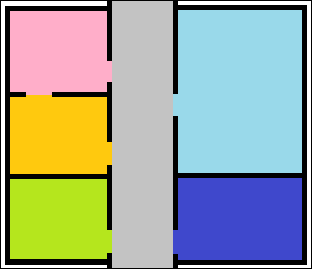
\includegraphics[width=\linewidth]{layout_alg}
\end{minipage}

\section[RFID]{De RFID opstellingen}
\label{ch:rfid}

\subsection{Statisch}

\subsubsection{1 antenne aan deurlijst}
\begin{minipage}{0.65\textwidth}
Deze opstelling is de eenvoudigste en 1 van de opstellingen die momenteel wordt gebruikt door Aucxis, ze is voornamelijk opgenomen in dit onderzoek als referentie. Het concept bij deze opstelling is dat aan elke deurlijst 1 RFID antenne hangt. Als er een tag voorbij de antenne gaat registreert deze dit en weten we dar er een beweging heeft plaatsgevonden. Of deze in of uit de locatie is kan niet uit deze data alleen afgeleid worden, dit kan enkel in combinatie met de informatie wat zijn locatie was voor de verplaatsing. Dit is een nadeel aan deze opstelling.
\end{minipage}
\hfill
\begin{minipage}{0.30\textwidth}
	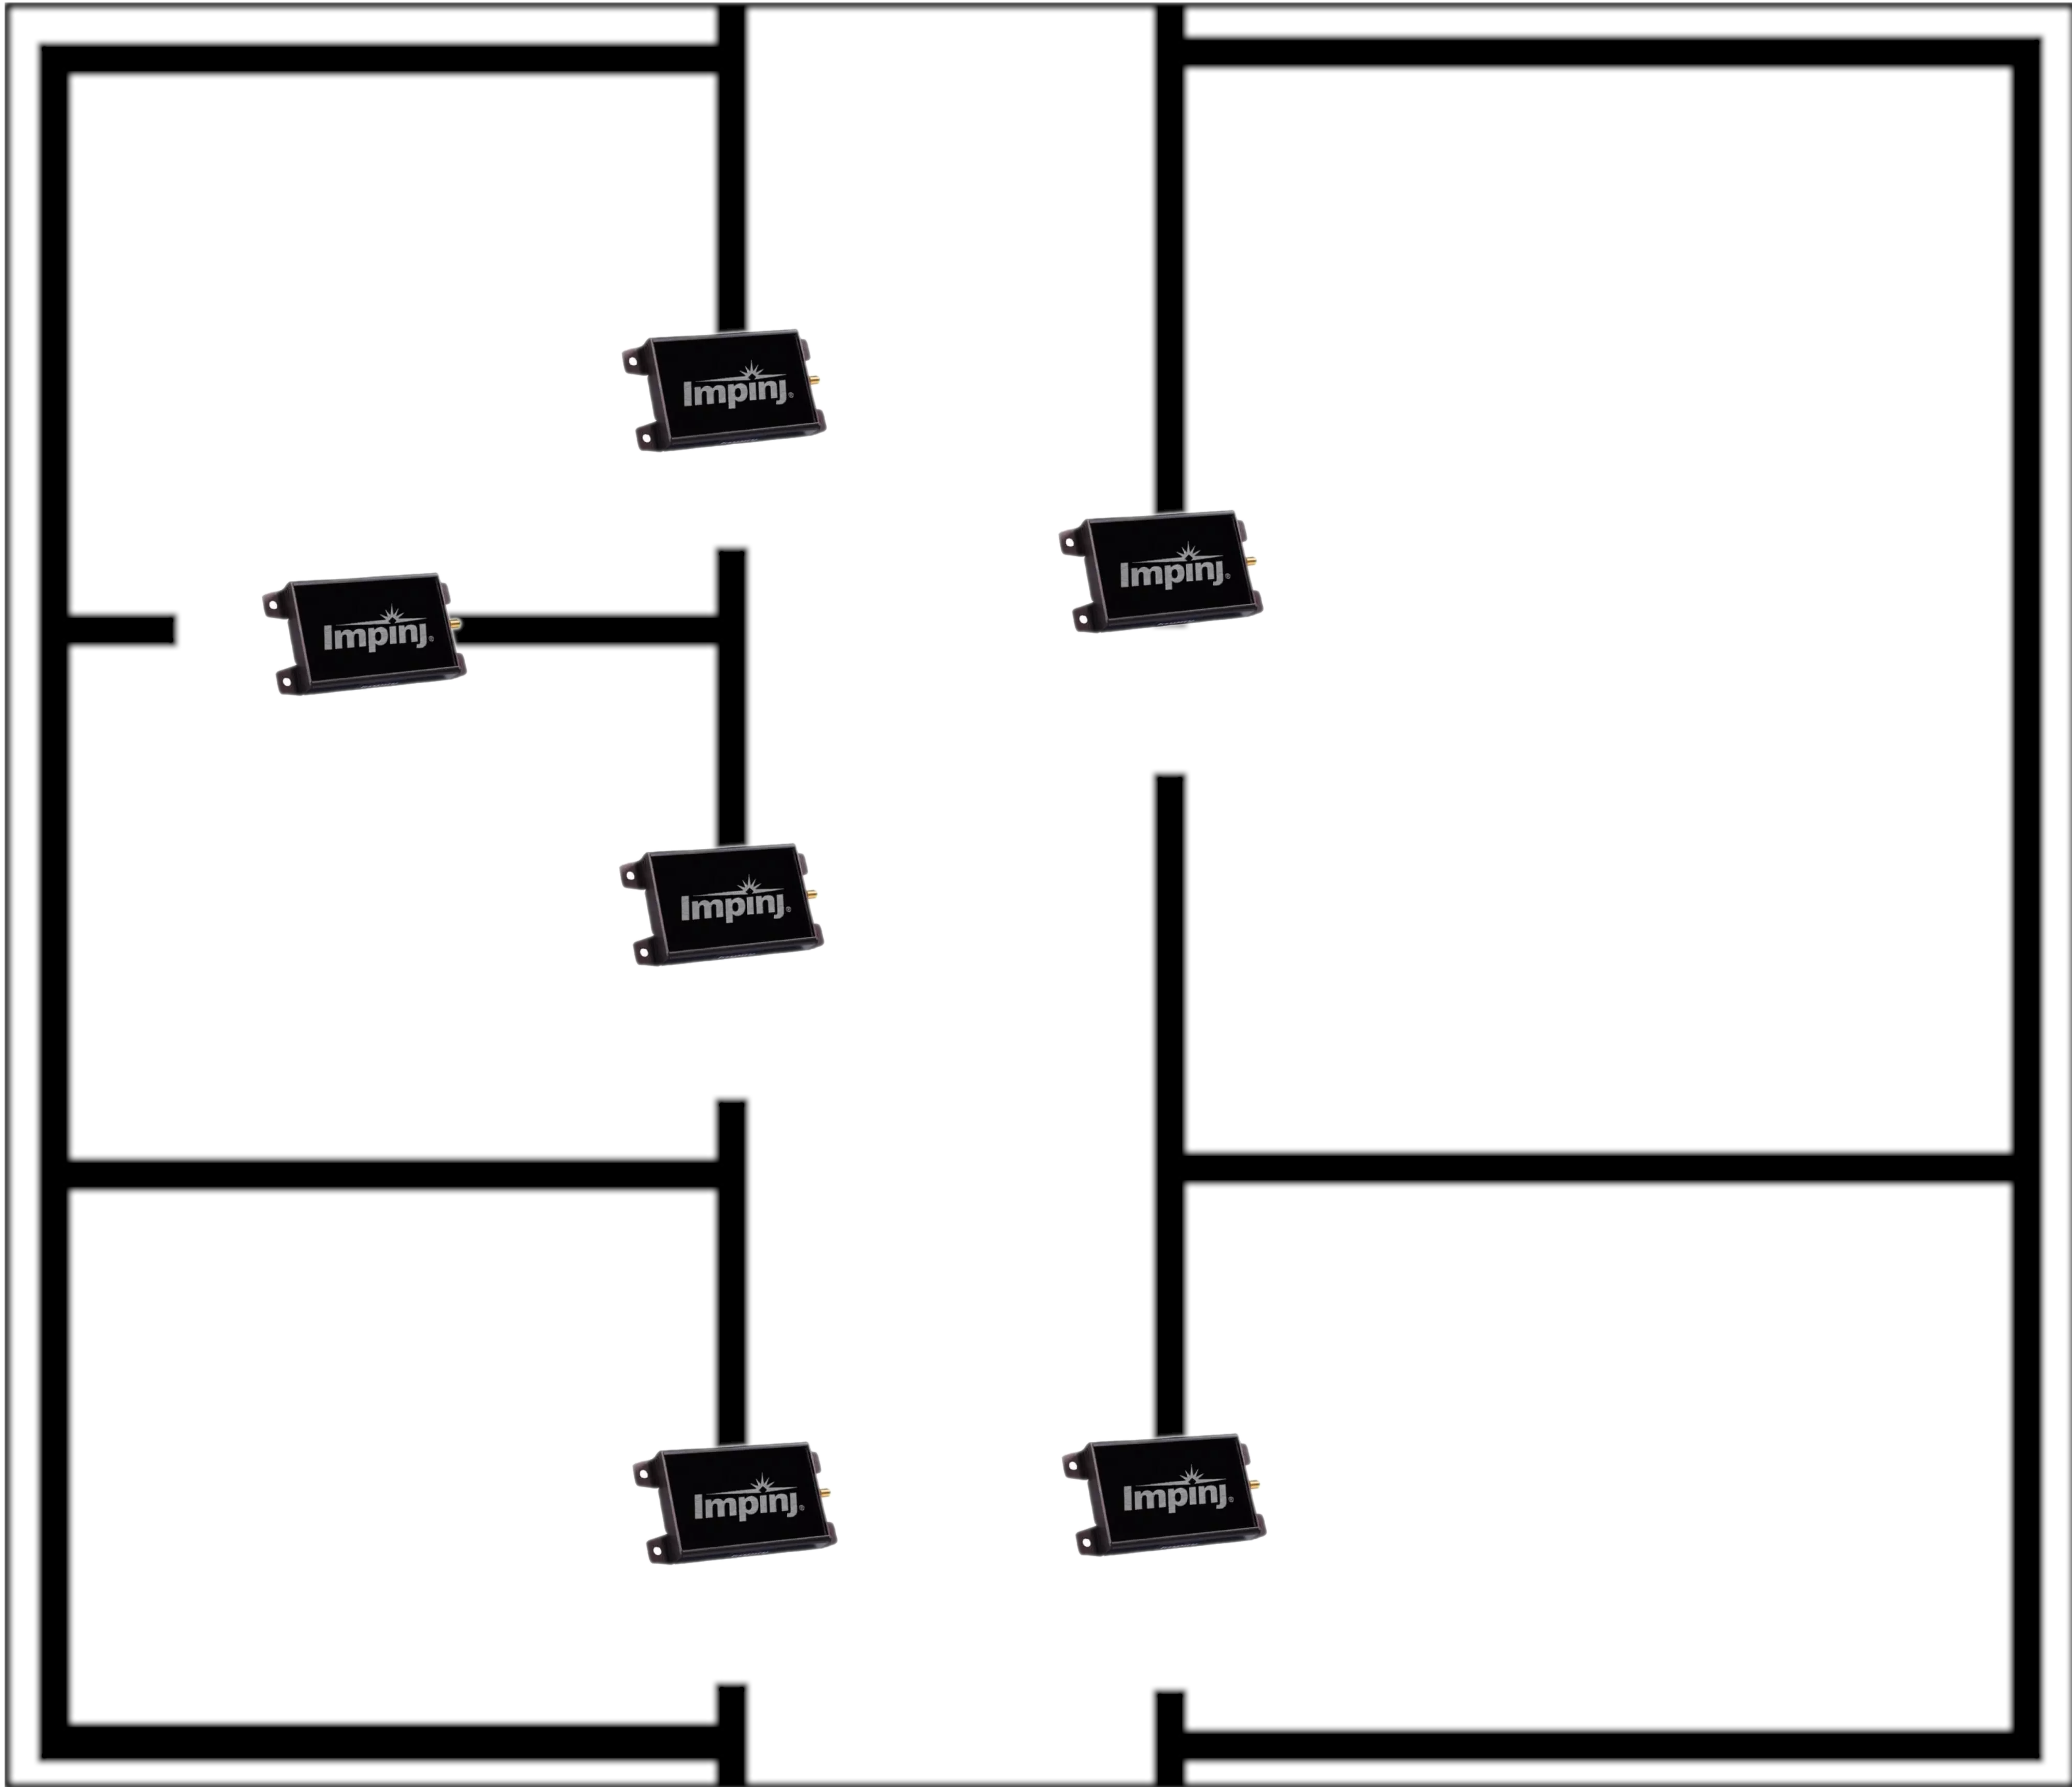
\includegraphics[width=\linewidth]{rfid_static_1}
\end{minipage}

\subsubsection{2 antenne aan deurlijst}
\begin{minipage}{0.65\textwidth}
Dit is ook 1 van de opstellingen die momenteel wordt gebruikt door Aucxis en dus ook voornamelijk een referentiepunt. Het principe is ongeveer hetzelfde als bij de vorige opstelling, echter is hier het voordeel dat de richting van de verplaatsing wel bekend is aan de hand van het tijdsverschil tussen de detecties van de tag. In dit opzicht is het dus beter dan de vorige opstelling, maar is uiteraard duurder door de hogere aantallen benodigde antennes. 
\end{minipage}
\hfill
\begin{minipage}{0.30\textwidth}
	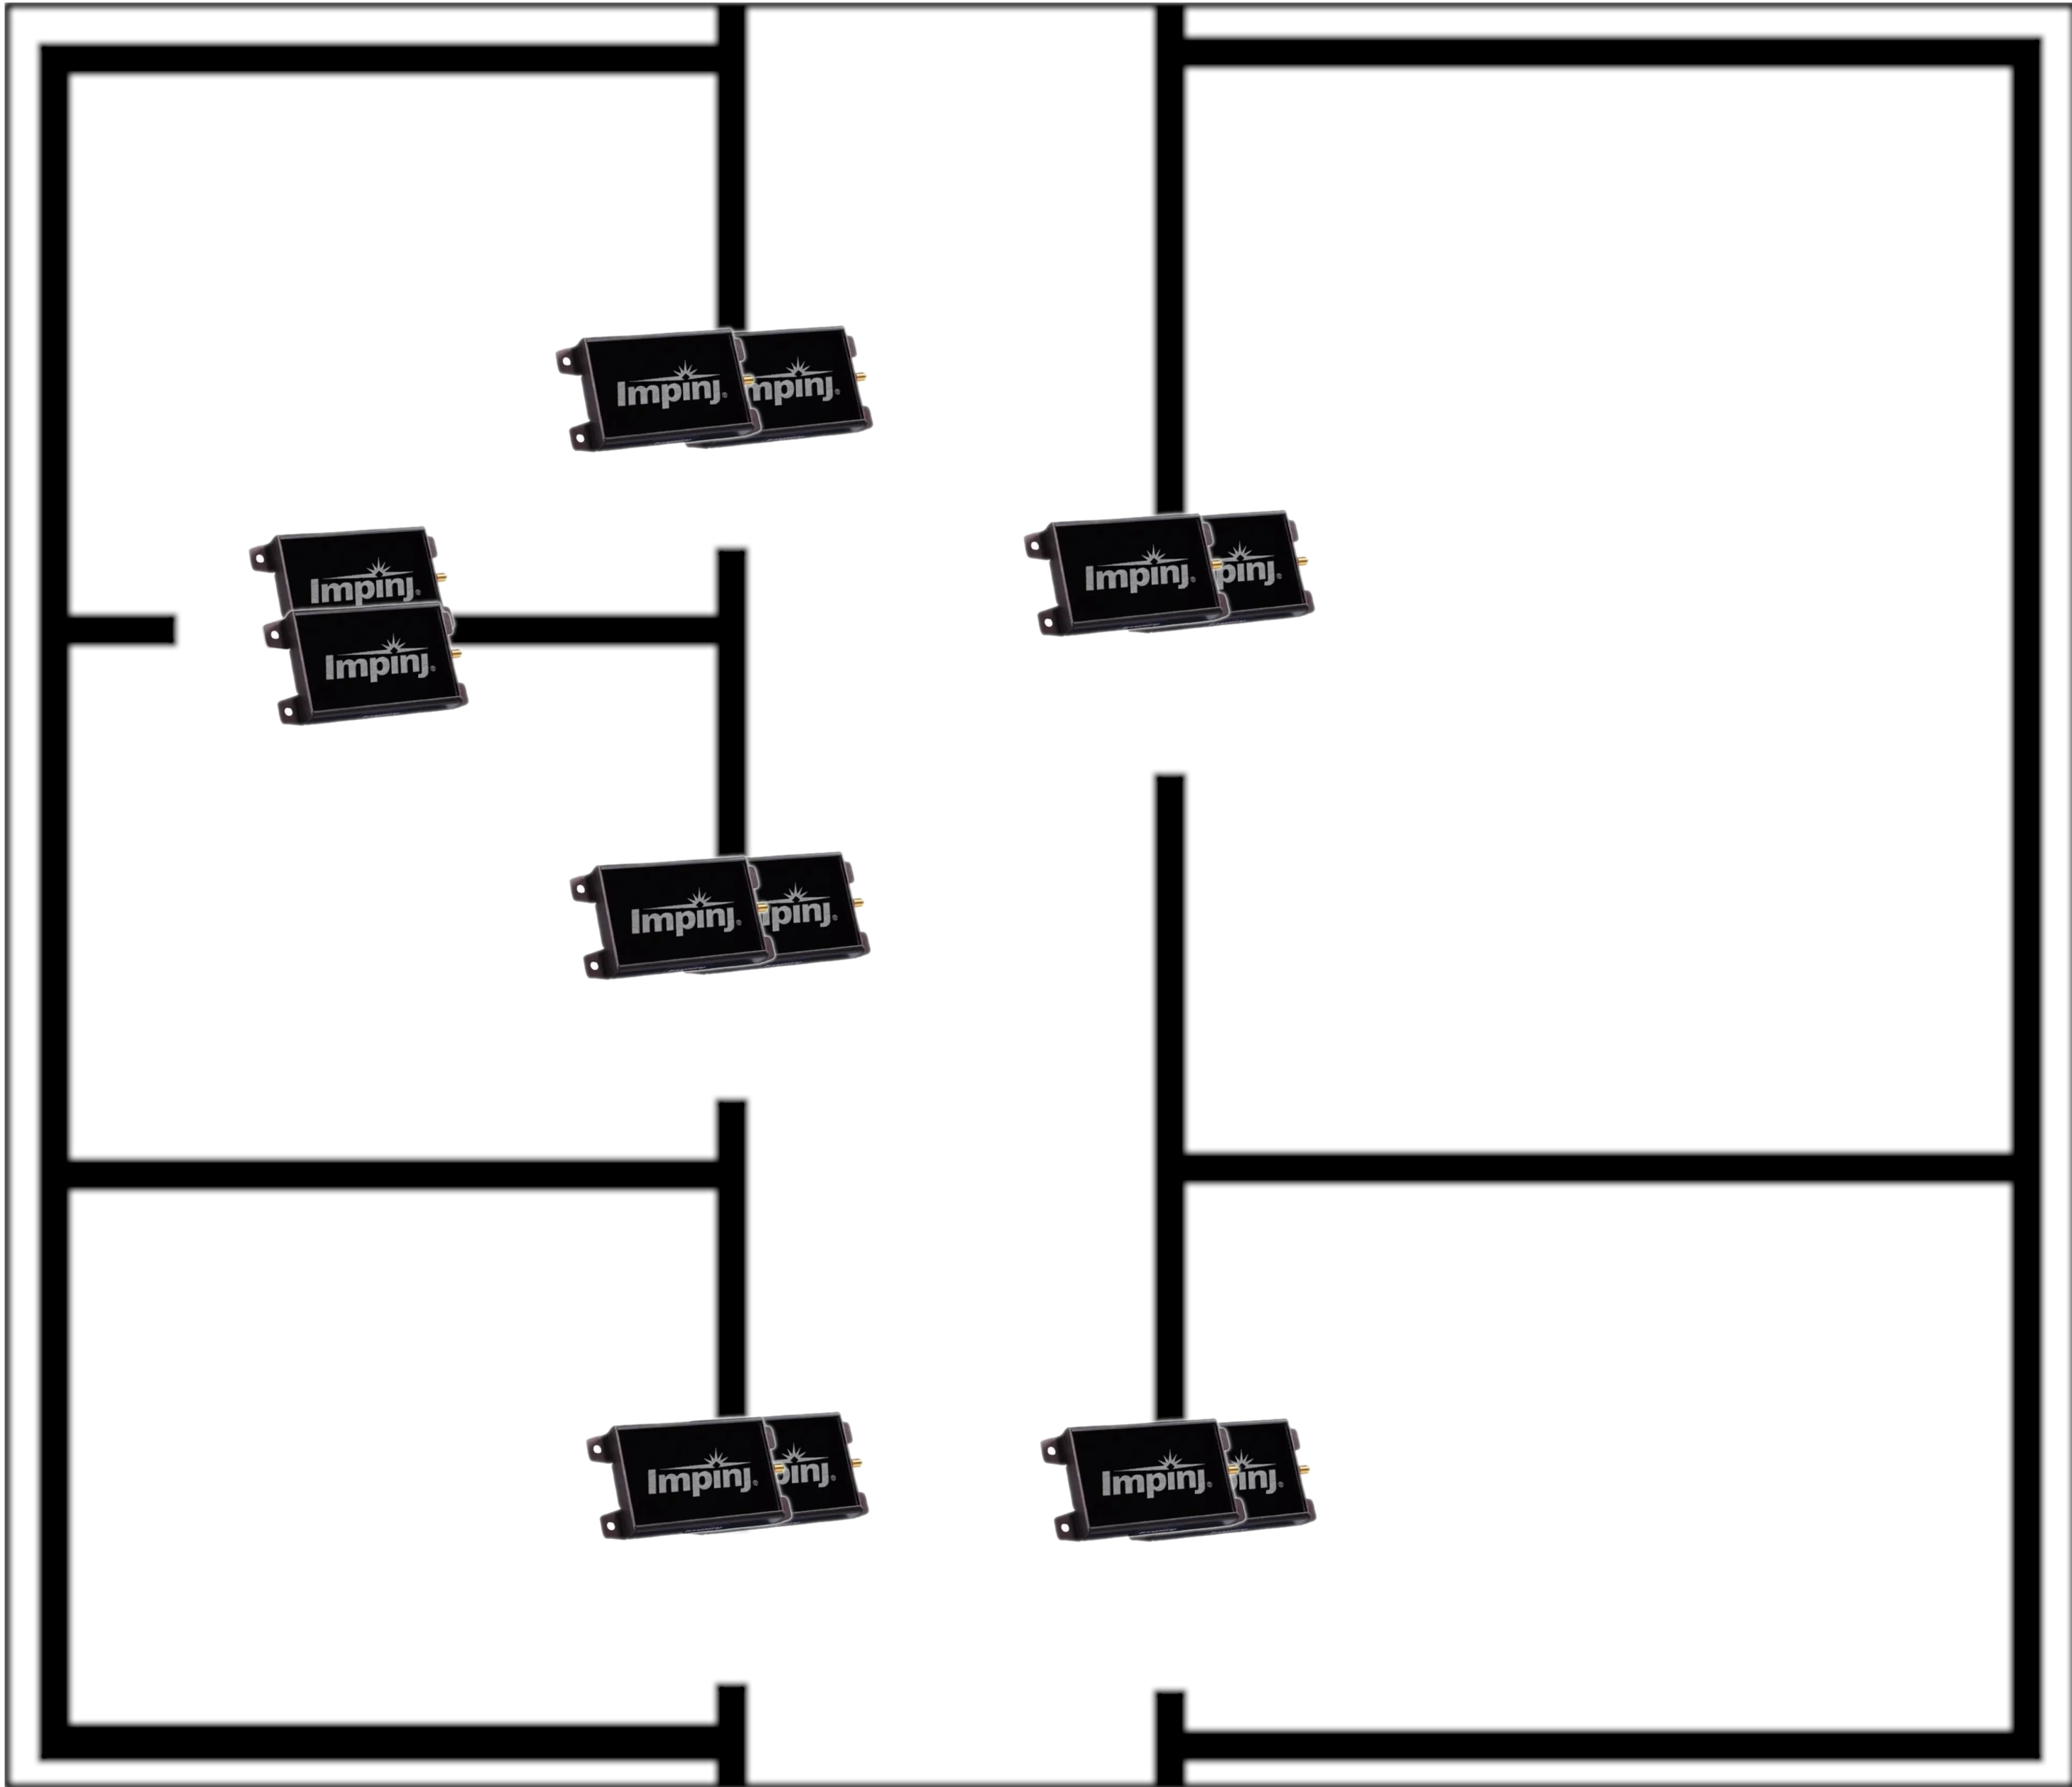
\includegraphics[width=\linewidth]{rfid_static_2}
\end{minipage}

\subsubsection{1 antenne tegenover deur}
\begin{minipage}{0.65\textwidth}
Bij deze opstelling wordt een RFID antenne tegenover de deur geplaatst, het idee hierachter is het feit dat, aangezien de RSSI afhankelijk is van de afstand tussen de antenne en de tag, het in theorie zichtbaar is aan de verandering in RSSI in welke richting de tag gaat. Ook geeft de antenne een doppler waarde mee, welke in theorie ook veranderd naargelang de richting. Als dit in praktijk blijkt te werken wilt dit zeggen dat er richtingsdetectie mogelijk is met 1 antenne, waardoor het sowieso al beter is dan de vorige 2 opstellingen. Nadeel is wel dat de kamer niet te breed mag zijn zodat de antenne ook tegenover de deur kan worden gemonteerd.
\end{minipage}
\hfill
\begin{minipage}{0.30\textwidth}
	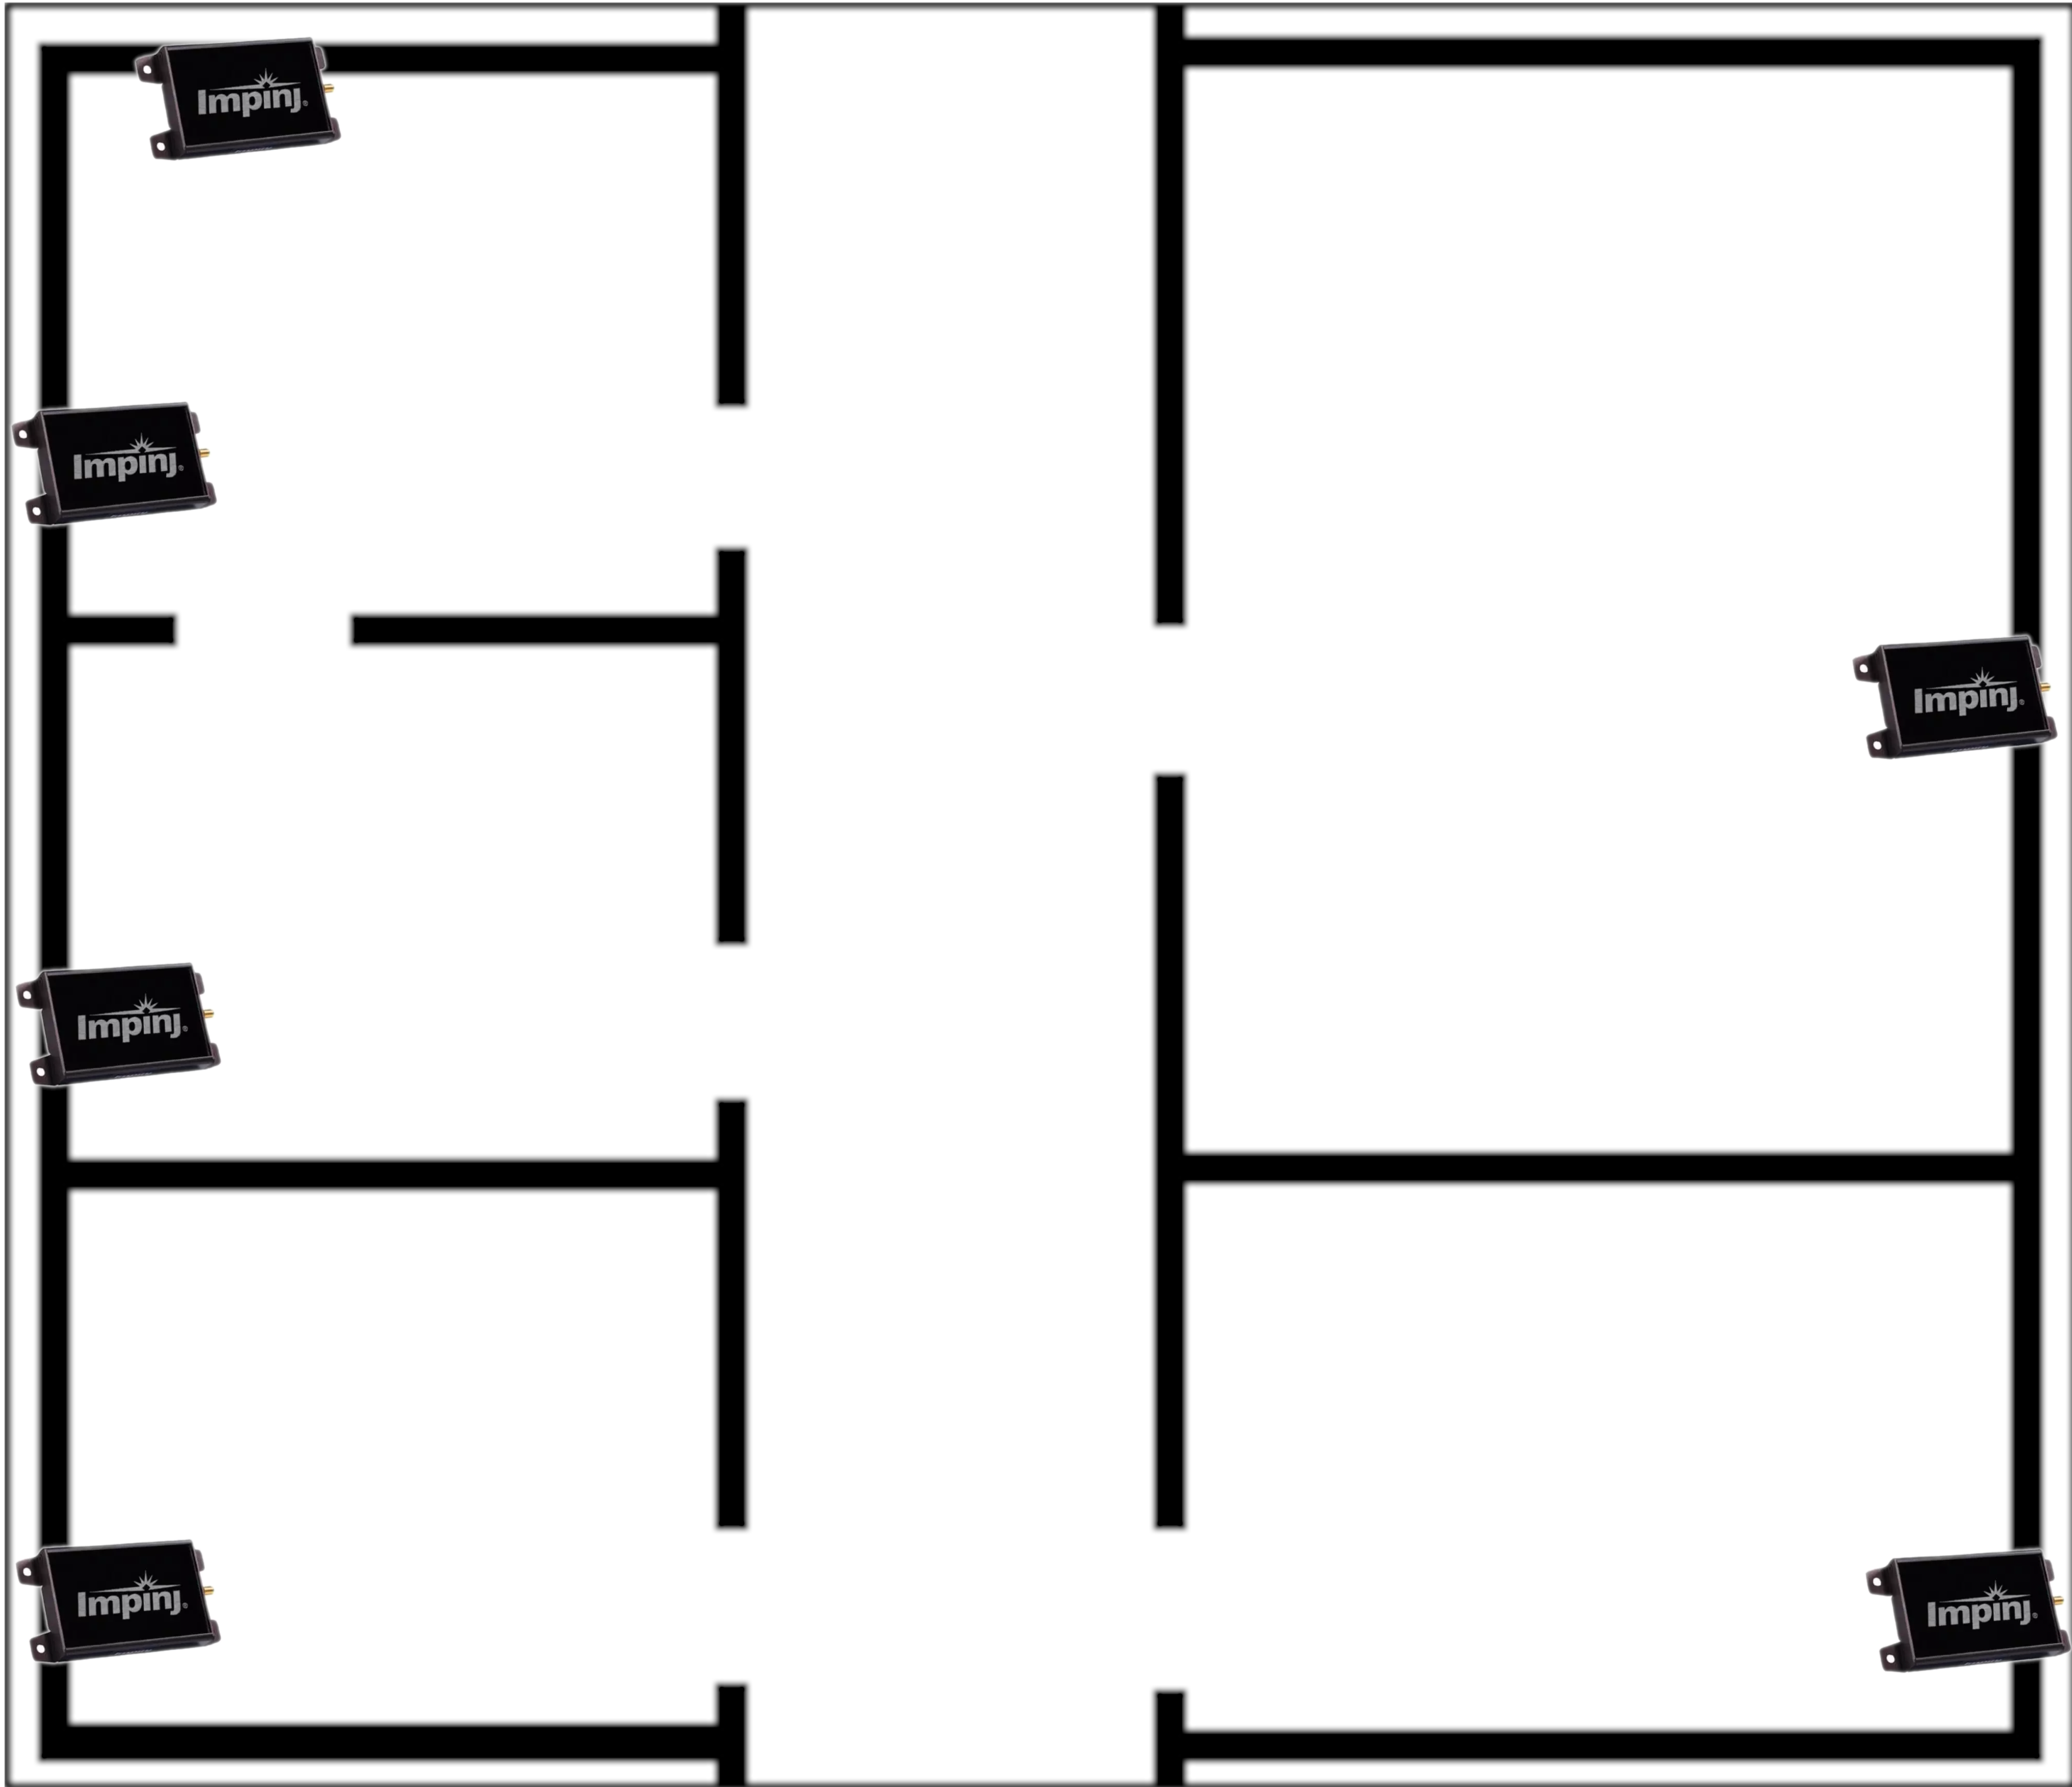
\includegraphics[width=\linewidth]{rfid_static_3}
\end{minipage}
\subsection{Dynamisch}

\subsubsection{1 tag aan deurlijst}
\begin{minipage}{0.65\textwidth}
Hier hangt er een RFID-tag aan de deurlijst (analoog aan de antenne bij de eerste statische opstelling). Als de antenne passeert aan de deur weet het aggregatieprogramma in theorie dat alle tags tussen nu en het passeren van deze of een andere locatie RFID-tag tot deze locatie behoren.
\end{minipage}
\hfill
\begin{minipage}{0.30\textwidth}
	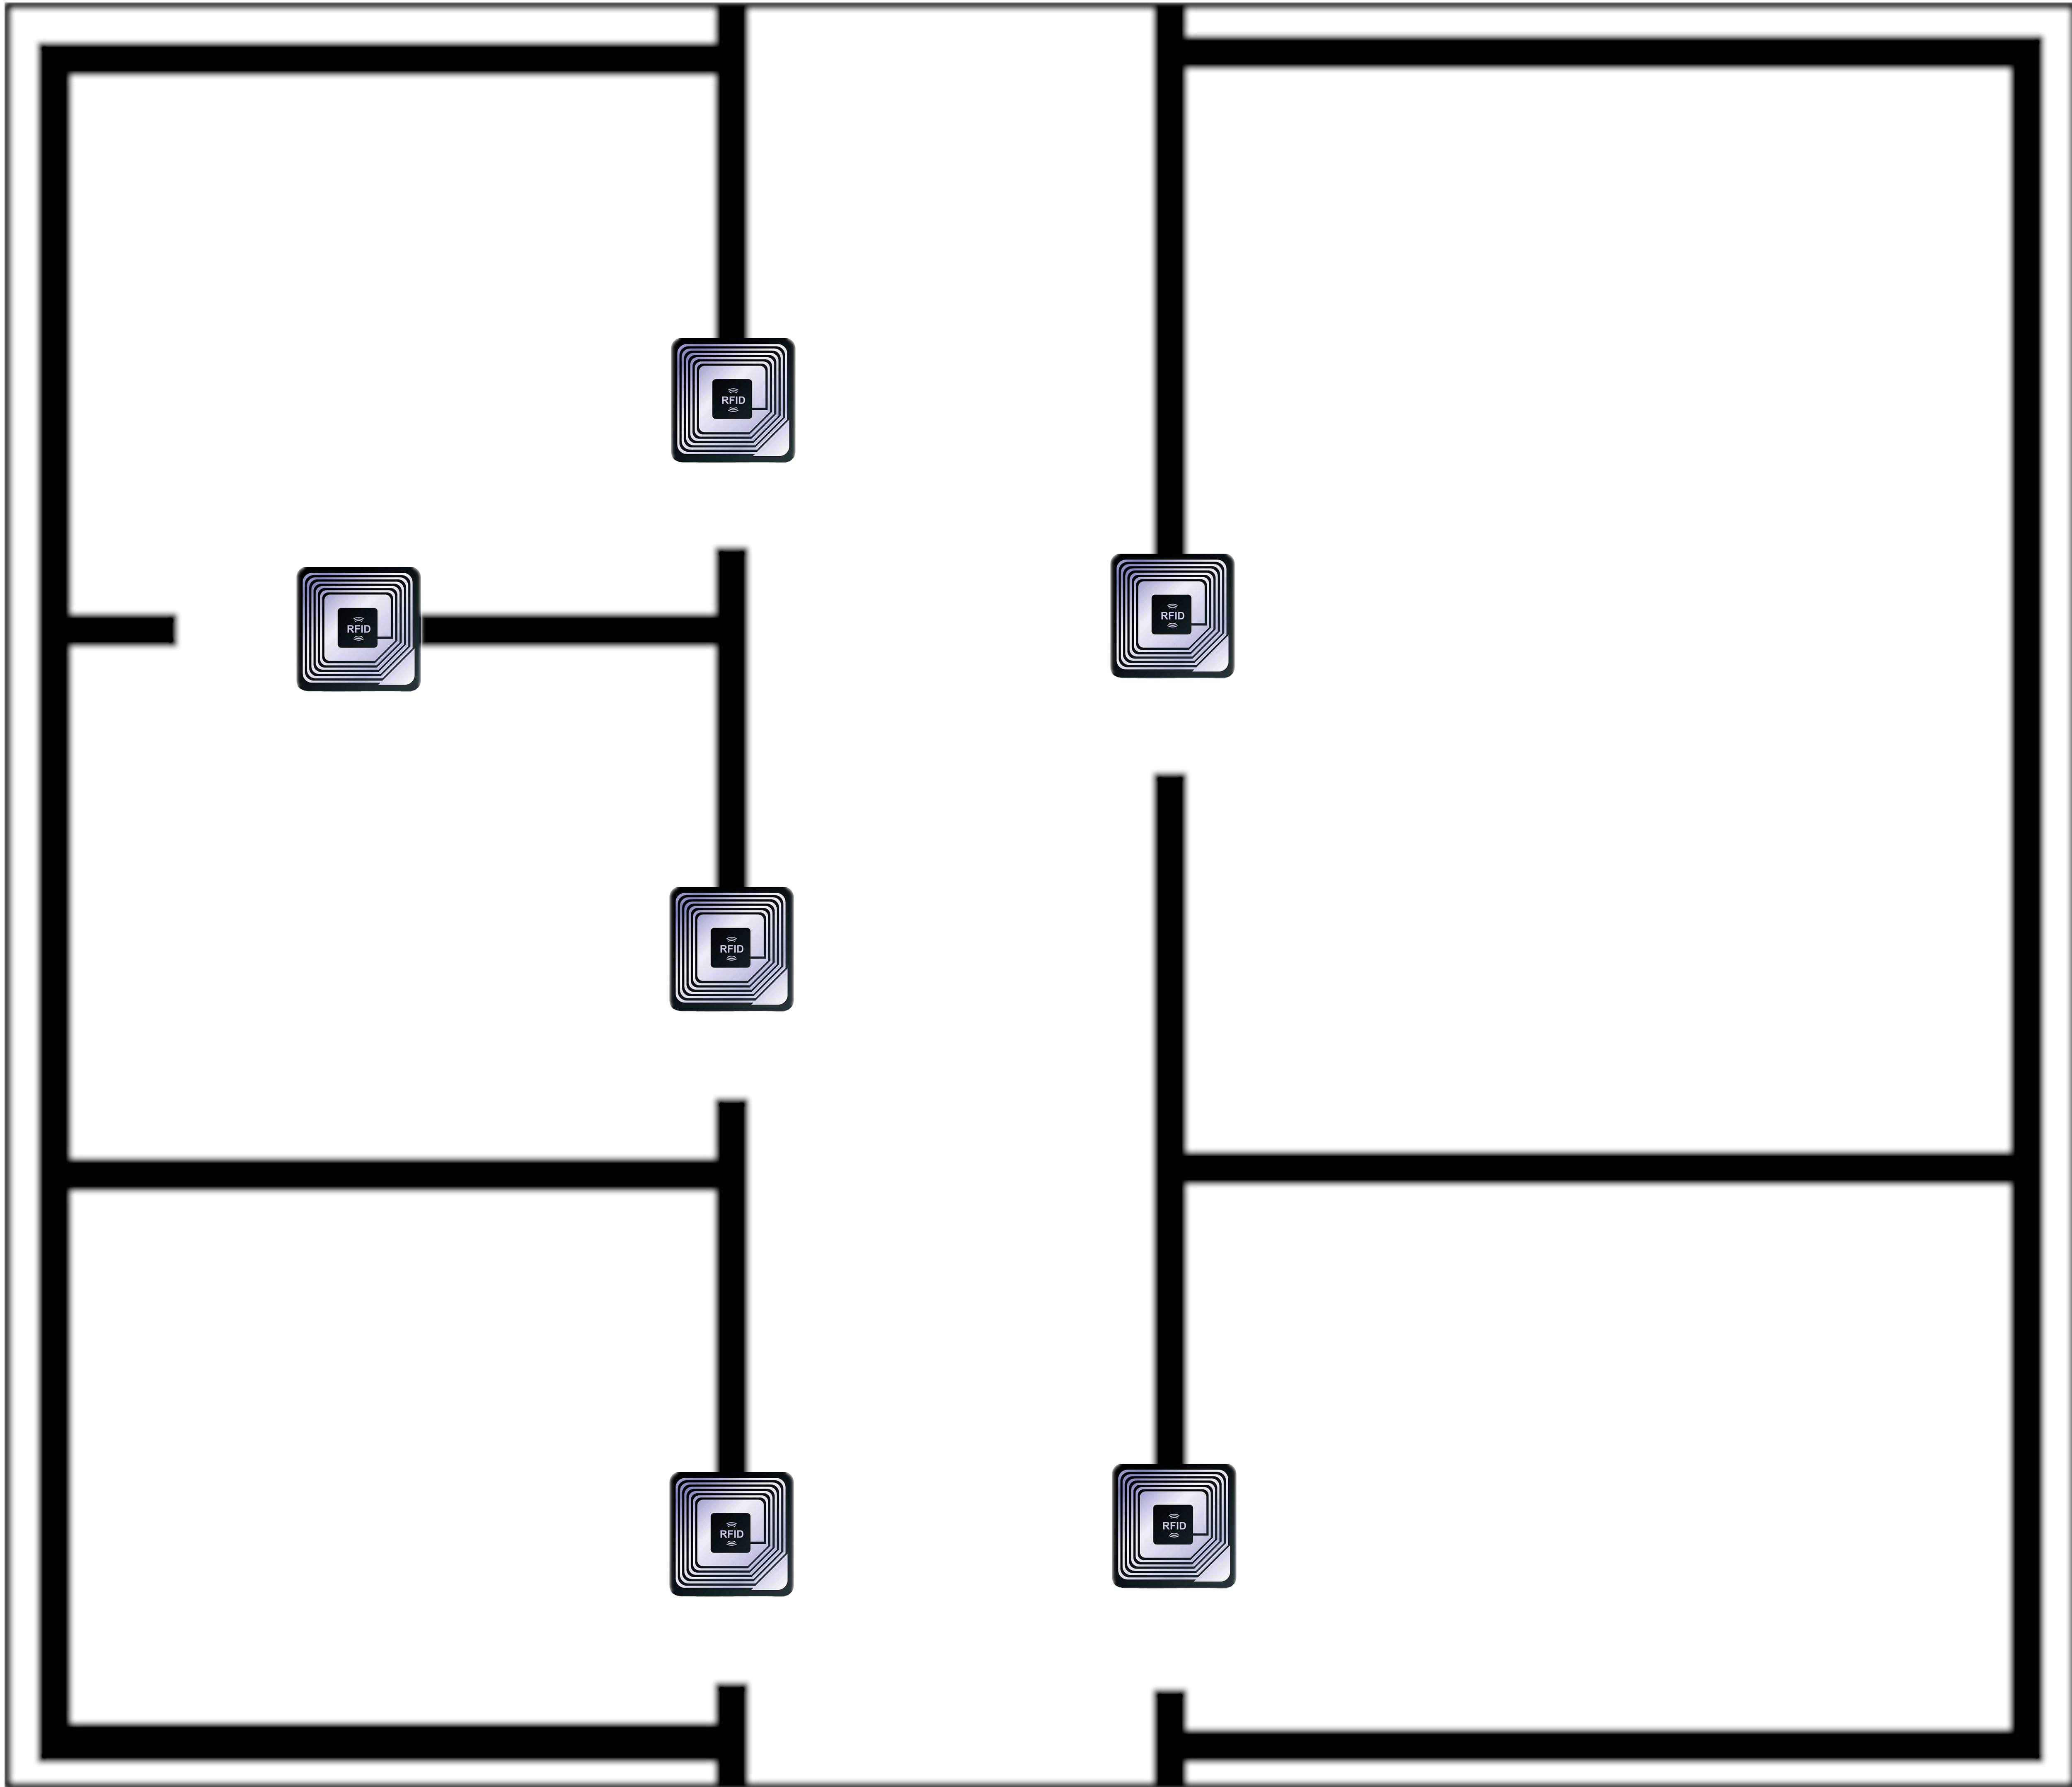
\includegraphics[width=\linewidth]{rfid_dynamic_1}
\end{minipage}

In theorie is het ook mogelijk de 2 andere statische scenario's een dynamische variant te geven, echter valt hun voordeel van richtingbepalend zijn weg hierbij aangezien de richting niet meer relevant is bij dynamisch. Deze worden dus buiten beschouwing gelaten.

\section[BLE]{De BLE opstellingen}
\label{ch:ble}

\subsection{Statisch}

\subsubsection{1 gateway per locatie}
\begin{minipage}{0.65\textwidth}
Deze opstelling is de eenvoudigste en meest intuïtieve van de BLE opstellingen. Elke locatie komt overeen met 1 IoT Gateway, die gepositioneerd wordt ongeveer in het middelpunt van de locatie. Het idee hierachter is dat de Gateway waar de beacon het dichtste bij is (de beste RSSI heeft), hoogstwaarschijnlijk de locatie is waar het voorwerp zich bevind. Dit is echter niet 100\% correct, en deze onnauwkeurigheid zal enkel maar groeien als de gateways/locaties onevenredig verdeeld zijn over de oppervlakte van het gebouw. 
\end{minipage}
\hfill
\begin{minipage}{0.30\textwidth}
	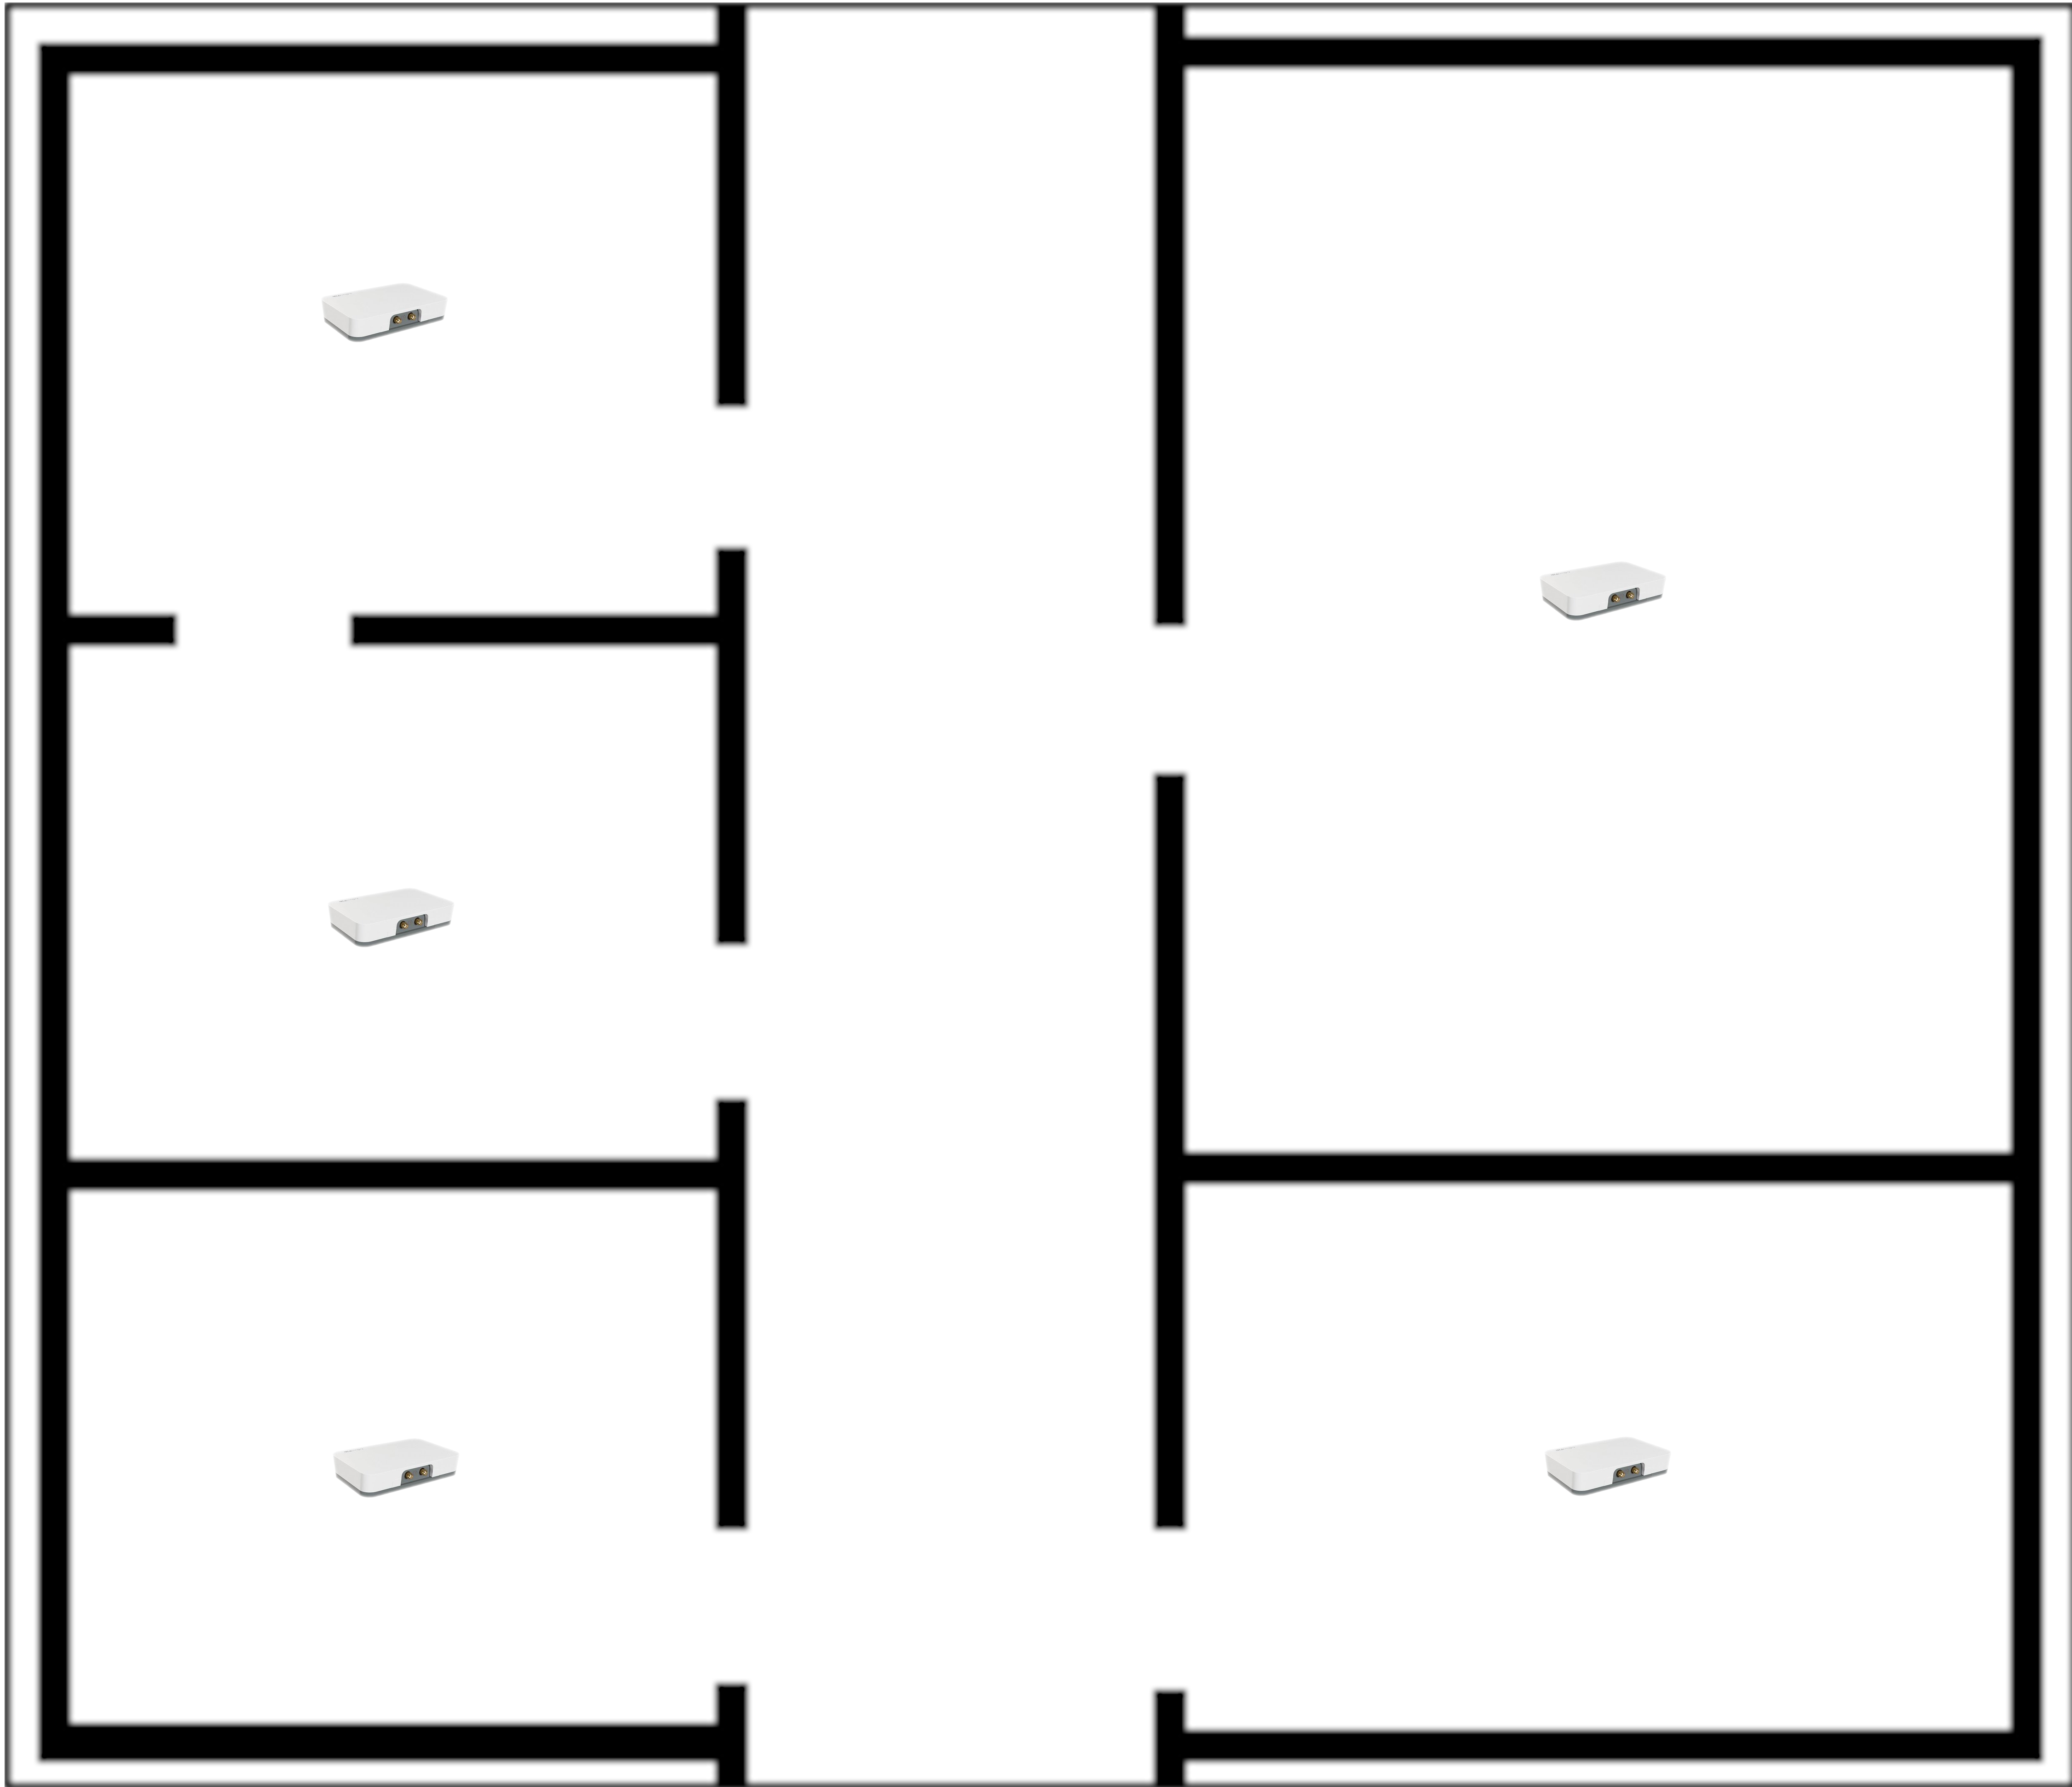
\includegraphics[width=\linewidth]{ble_statisch_1}
\end{minipage}

\subsubsection{Meerdere gateways per locatie}
\begin{minipage}{0.65\textwidth}
In deze opstelling wordt een locatie gedefinieerd door meer dan 1 gateway, nl. een gateway per hoek van de locatie, zodat de locatie wordt omringd door een kader van gateways. Hiermee kan in theorie zeer gedetailleerd worden afgeleid waar de beacon zich bevind, maar de kost voor de opstelling vliegt vrij snel de hoogte in als er veel locaties zijn. Wel kunnen gedeelde hoeken van locaties door een gedeelde beacon worden bezet.
\end{minipage}
\hfill
\begin{minipage}{0.30\textwidth}
	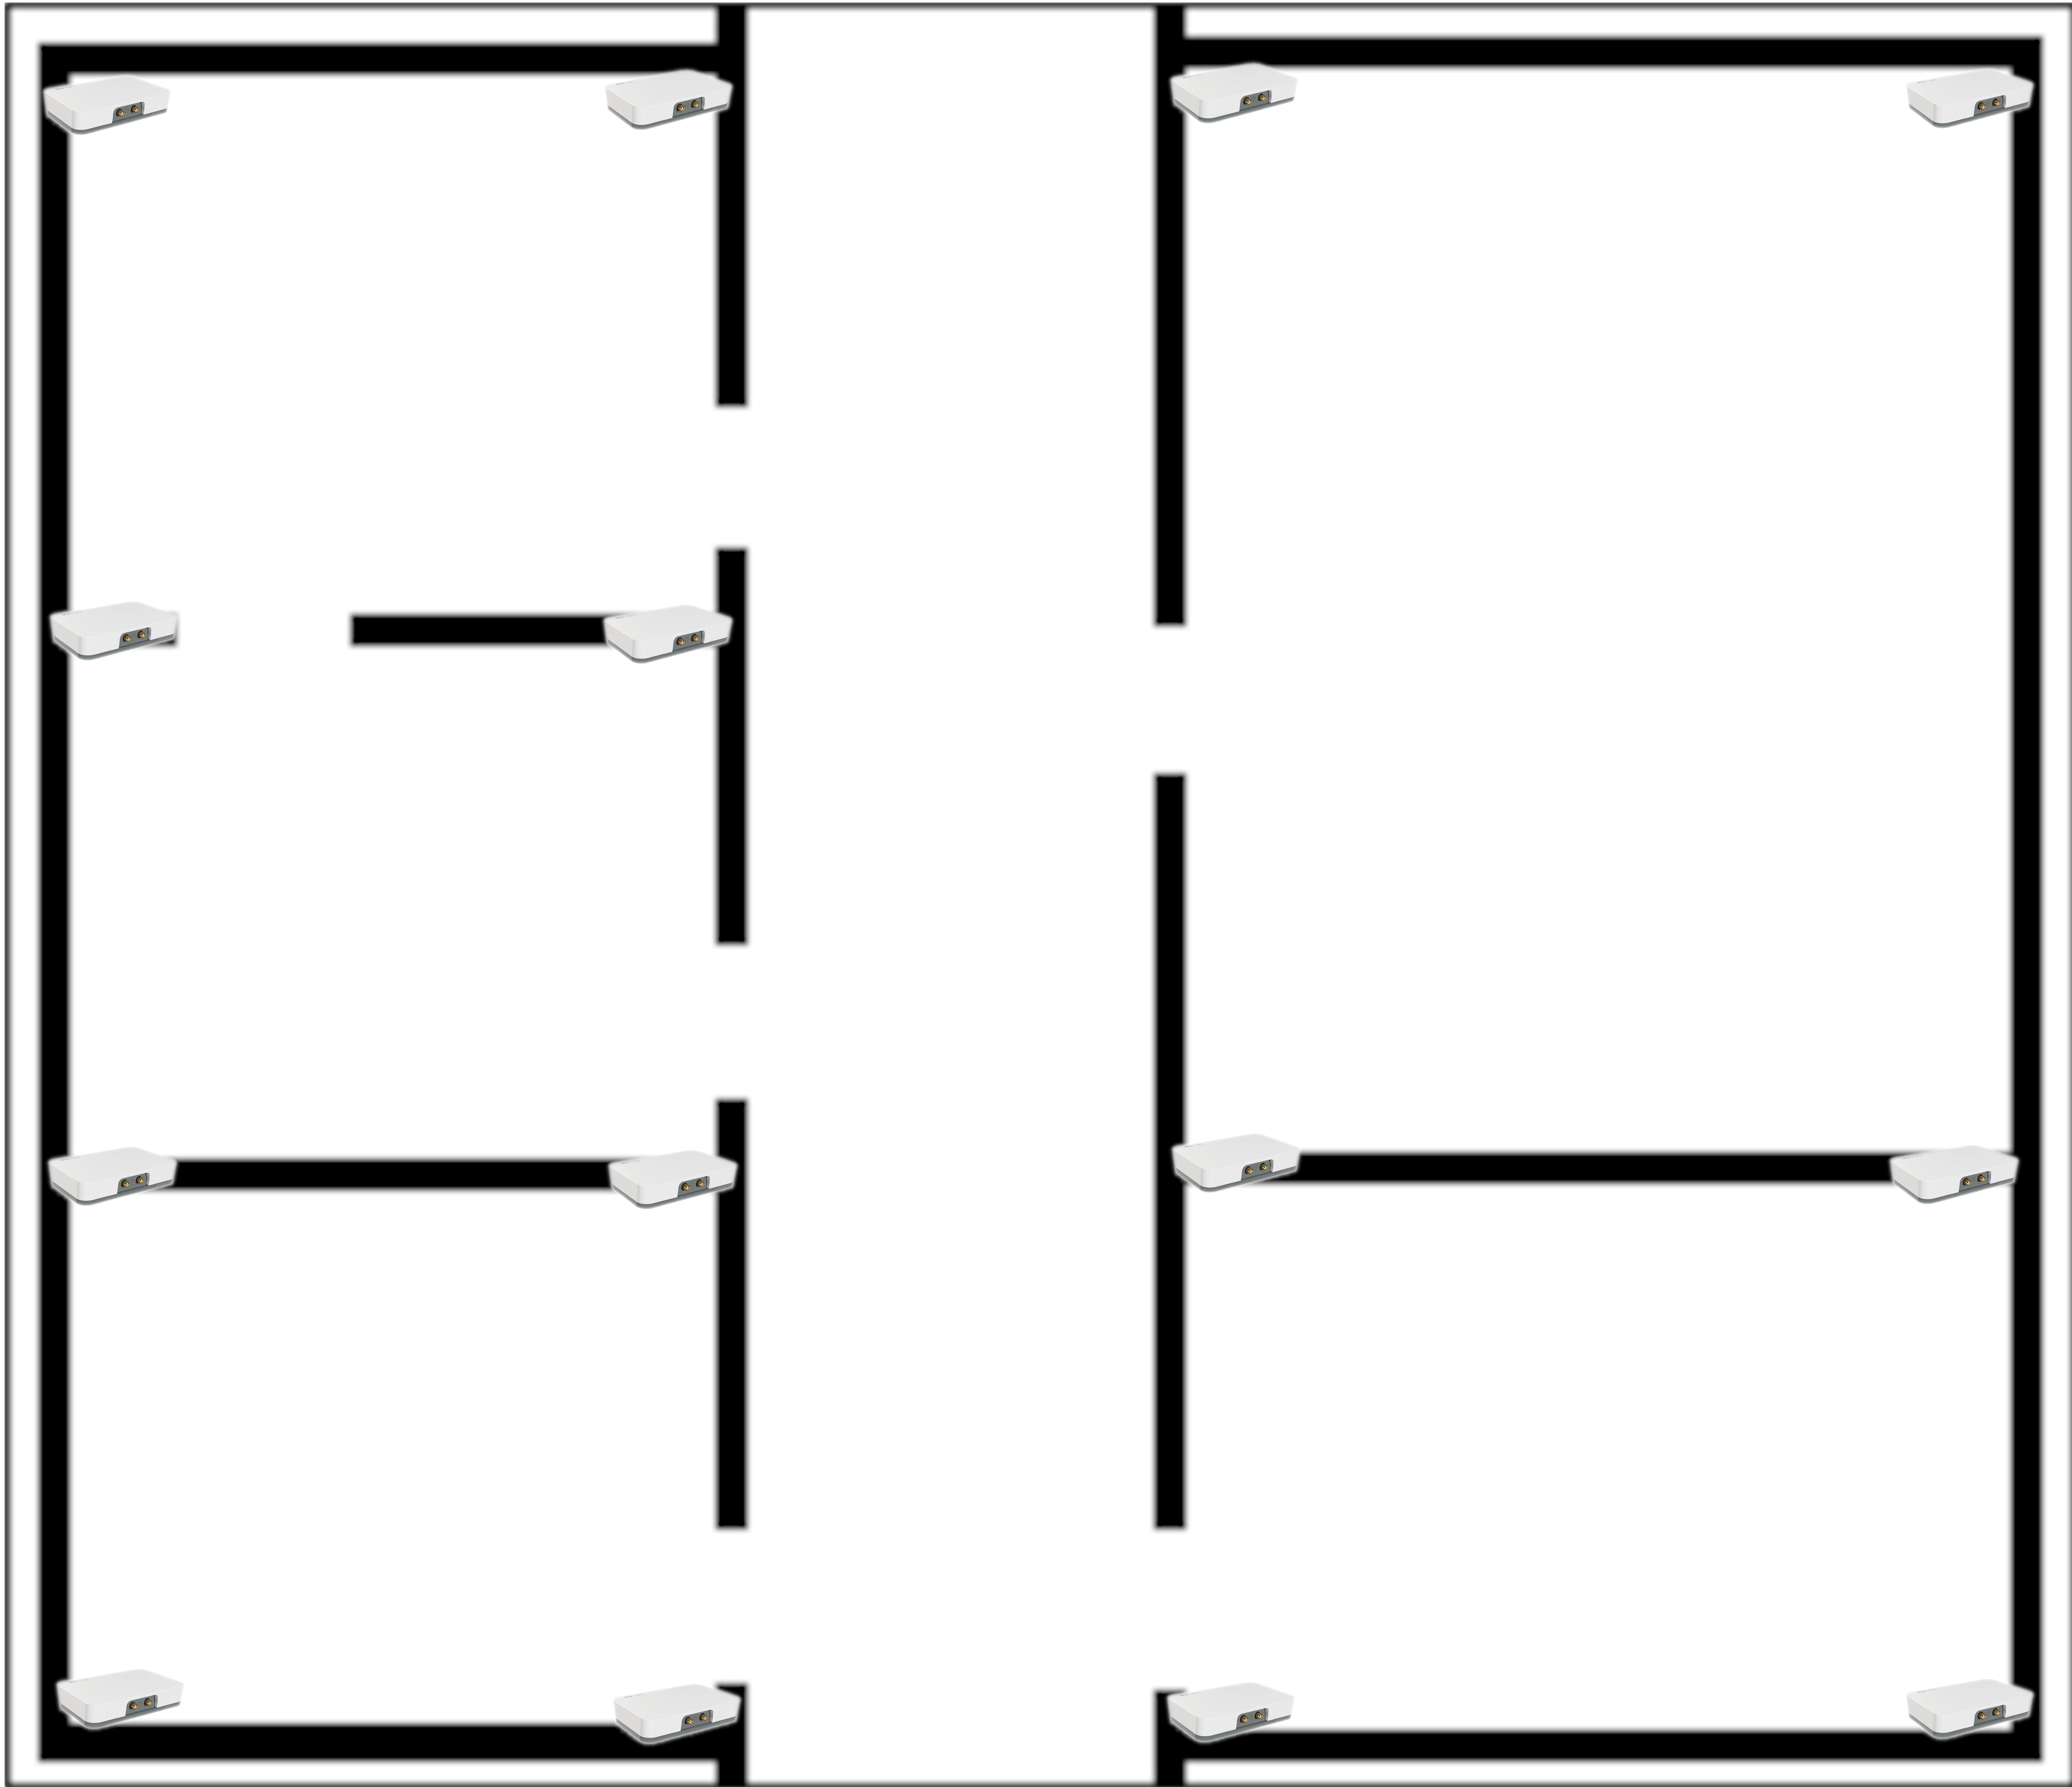
\includegraphics[width=\linewidth]{ble_statisch_2}
\end{minipage}

\subsubsection{Rasteropstelling}
\begin{minipage}{0.65\textwidth}
Deze opstelling bestaat uit een raster welke volledig het gebouw omvat. Als de locaties van deze gateways bekend zijn kan via trigonometrie en de gemeten RSSI waardes berekend worden waar de voorwerpen zich bevinden, wat dan gelinkt kan worden aan een locatie. Dit is vrij precies en schaalt goed, maar nadelig is wel dat de locaties volledig gespecificeerd en bijgehouden moeten worden want er kan niet enkel op data van de gateways worden afgegaan om de locatie te bepalen aangezien de gateways en de locaties niks meer met elkaar te maken hebben.
\end{minipage}
\hfill
\begin{minipage}{0.30\textwidth}
	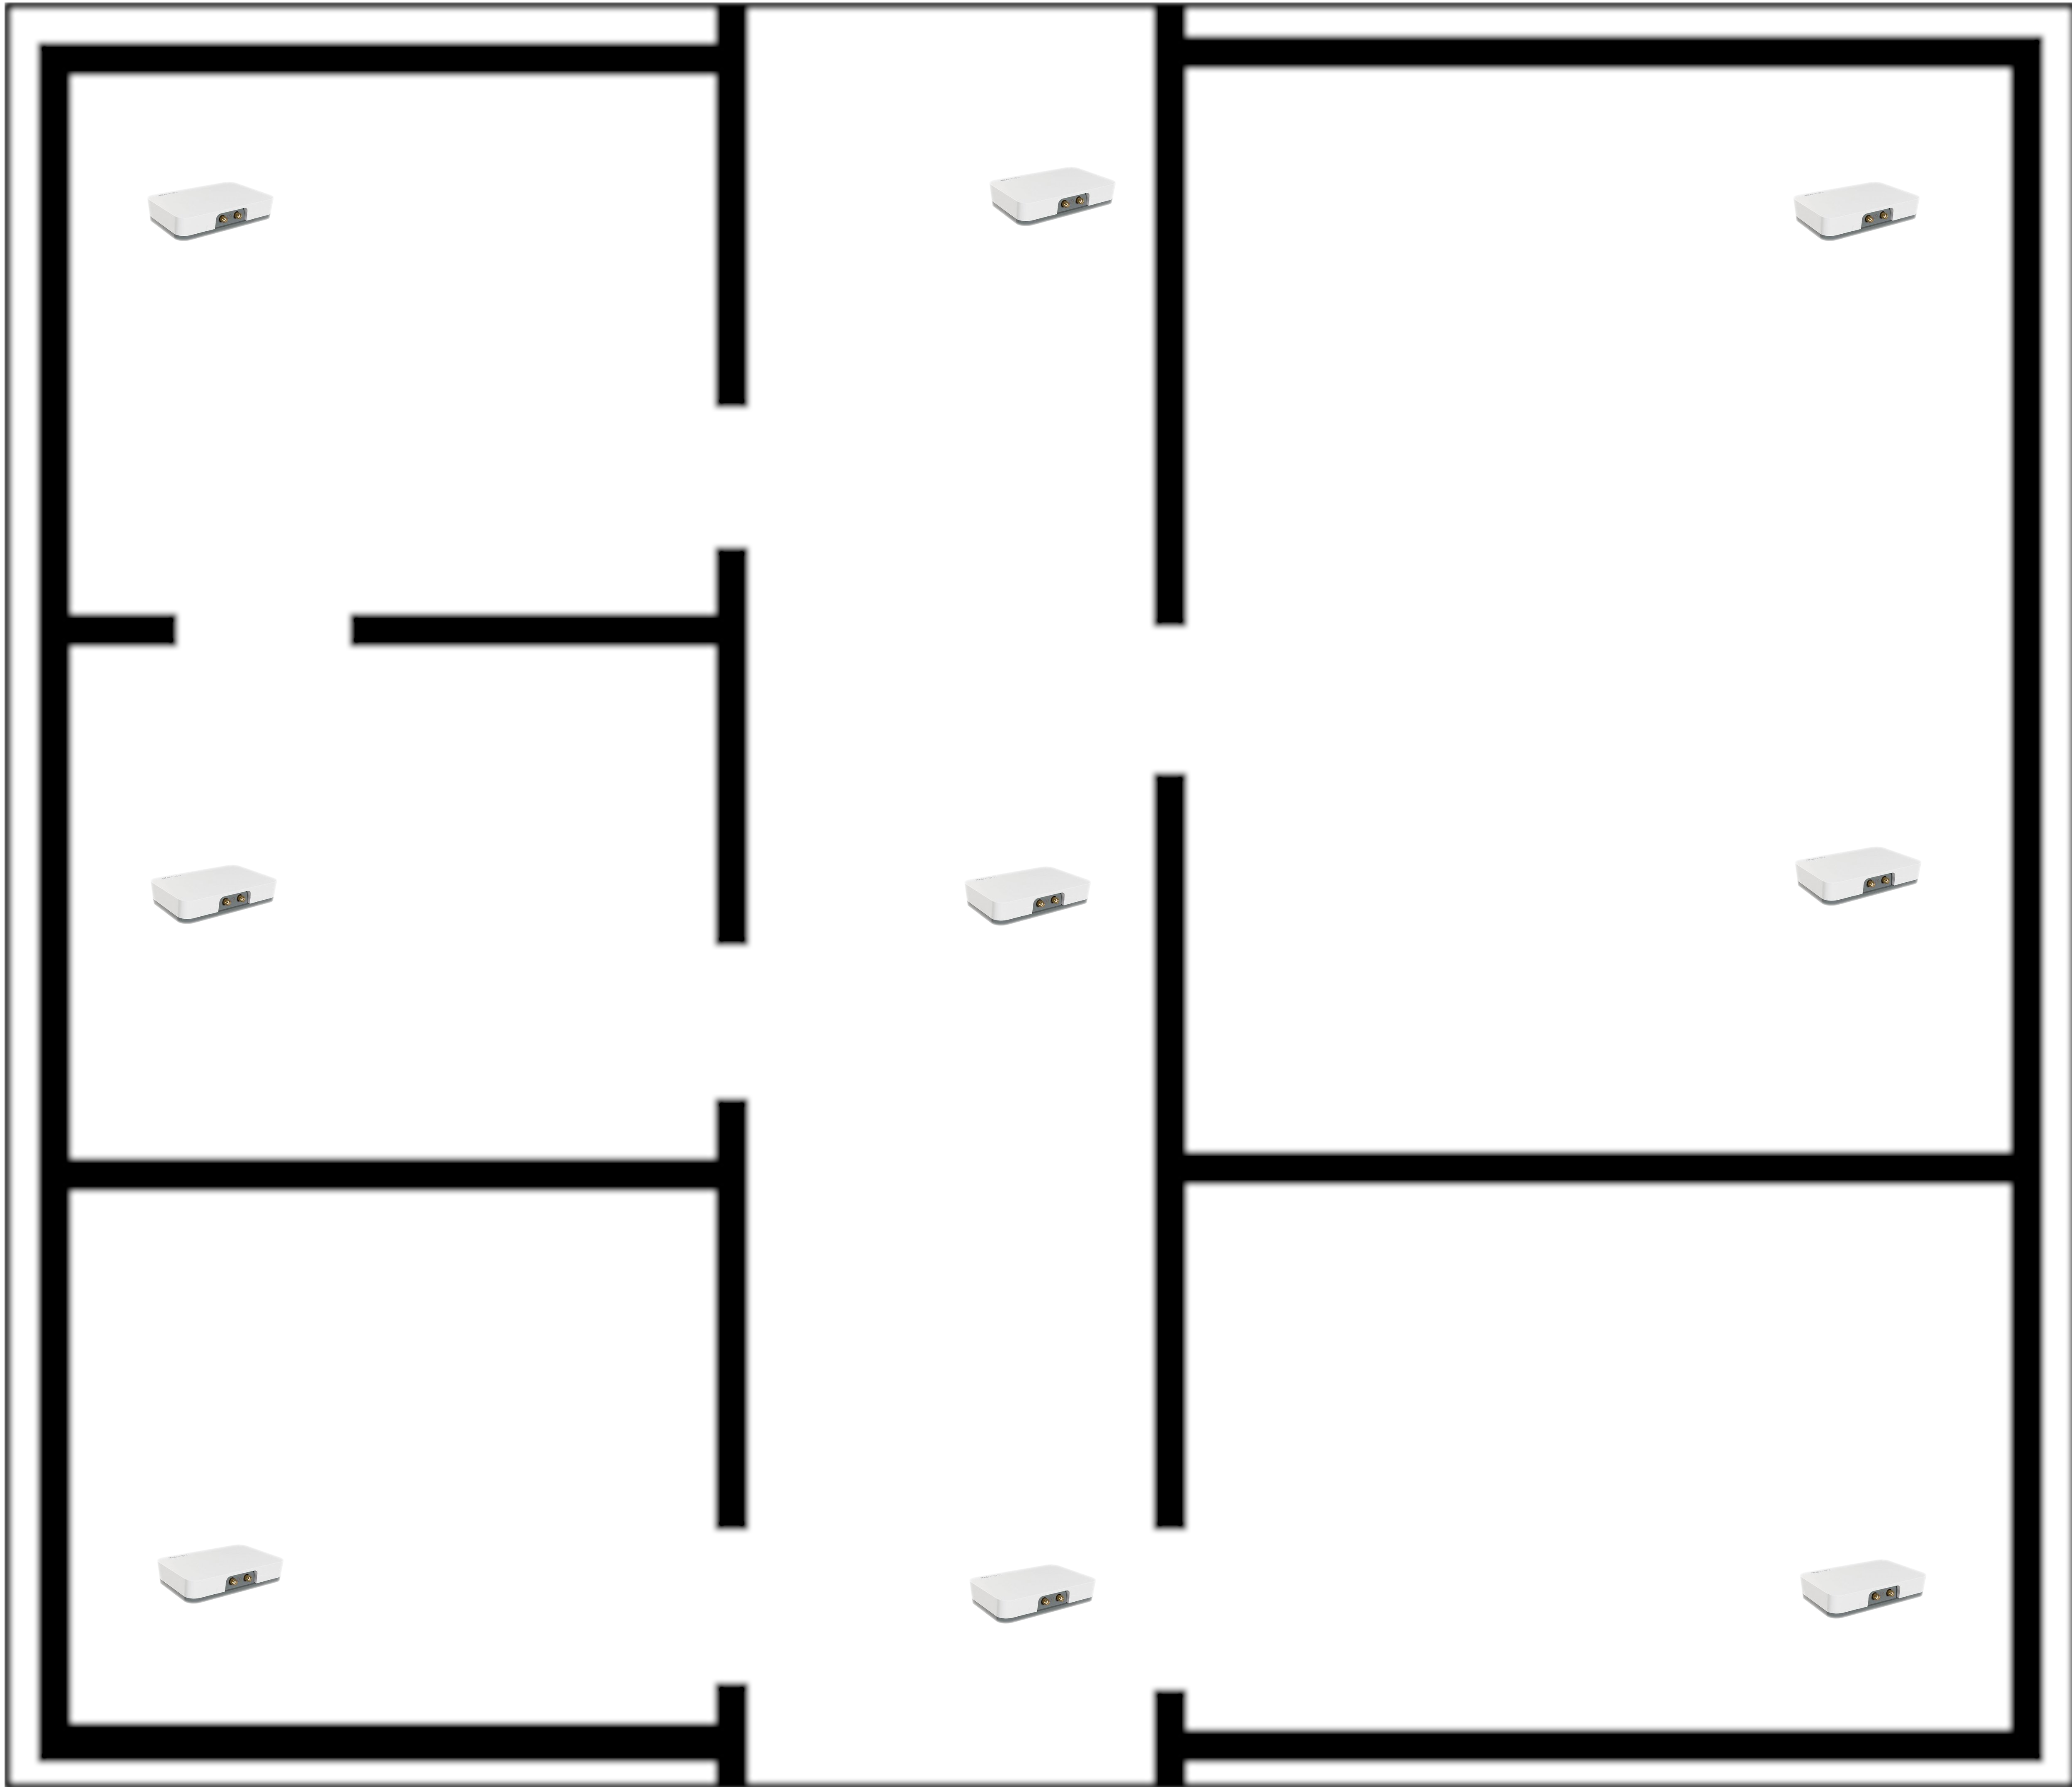
\includegraphics[width=\linewidth]{ble_statisch_3}
\end{minipage}


\subsection{Dynamisch}

\subsubsection{1 beacon per locatie, midden van kamer}
%TODO

\subsubsection{1 beacon per locatie, aan deur}
%TODO

\subsubsection{< 1 beacon per locatie}
%TODO

\subsubsection{> 1 beacon per locatie}
%TODO

\subsubsection{beacons op intervallen in de gang}
%TODO

% Voeg hier je eigen hoofdstukken toe die de ``corpus'' van je bachelorproef
% vormen. De structuur en titels hangen af van je eigen onderzoek. Je kan bv.
% elke fase in je onderzoek in een apart hoofdstuk bespreken.

%%=============================================================================
%% Methodologie
%%=============================================================================

\chapter{\IfLanguageName{dutch}{Methodologie}{Methodology}}
\label{ch:methodologie}

%% TODO: Hoe ben je te werk gegaan? Verdeel je onderzoek in grote fasen, en
%% licht in elke fase toe welke stappen je gevolgd hebt. Verantwoord waarom je
%% op deze manier te werk gegaan bent. Je moet kunnen aantonen dat je de best
%% mogelijke manier toegepast hebt om een antwoord te vinden op de
%% onderzoeksvraag.

Het hoofddoel, namelijk het bepalen van een optimale hardwareopstelling, zal in eerste instantie opgedeeld worden in enkele deelonderzoeken, 1 deelonderzoek per hardwareopstelling. Elk deelonderzoek zal verder onderverdeeld worden in een deelhypothese (Hoe de opstelling in theorie zou moeten presteren, opgebouwd uit veronderstellingen en theoretische waarheden aangehaald in Hoofdstuk~\ref{ch:literatuurstudie}), enkele experimenten, en een deelconclusie. Deze deelconclusie zal een vergelijking zijn tussen de hypothese en de eigenlijke uitkomst, een opsomming van de voor- en nadelen, een categorisatiescore (Hoeveel procent van de gemeten beacons kan juist geplaatst worden aan de hand van de data en het lokalisatieprincipe) en een uiteenzetting over de factoren die al dan niet aanwezig moeten zijn om het principe acceptabel te maken. Ten slotte zullen de deelconclusies vergeleken worden en zal er een algemene conclusie bepaald worden. De onderzochte opstellingen, 12 in totaal, zijn hoogstwaarschijnlijk niet alle mogelijke manieren waarop de onderzoeksopzet, namelijk het registreren van verplaatsingen, kan gebeuren. De bepaling van deze set zijn het resultaat van een overleg met Aucxis welke opstellingen het meest kans hebben om te werken, en het interessantst zijn voor hen om onderzocht te zien. Voor de oplijsting van deze opstellingen, samen met een korte theoretische achtergrond verwijs ik de lezer naar Hoofdstuk~\ref{ch:opstellingen}.

Voordat er experimenten kunnen gebeuren is het belangrijk een oplijsting te maken van enkele constanten doorheen het onderzoek. Voornamelijk op het vlak van de gebruikte hardware en de standaardinstellingen waarmee dit onderzoek zal gebeuren. Deze constanten zijn geldig gedurende het volledige onderzoek, tenzij anders aangegeven.

\section{RFID}
Voor de RFID opstellingen wordt gebruik gemaakt van KEONN Advantenna-p11 antennes, dit zijn vlakke, wide beam antennes. Ze stralen dus voor zich uit met een relatief wijd veld van 90° volgens zowel de x- als y-as \autocite{Keonn}. Deze zijn dus ideaal om te bepalen of er een tag voor de antenne passeert.
Als tranceiver wordt een 4-port IMPINJ Speedway Revolution gebruikt, deze maakt het mogelijk om 4 antennes tegelijk aan te sluiten. De gebruikte tags zijn standaard RFID tags van ~9 x 1.5cm, met 1 antenne in 1 richting. Verder zenden de antennes een EM veld uit met Tx = 20dB. De resultaten van de test worden opgevangen en gevisualiseerd met ARTA.

\section{BLE}
In de BLE opstellingen wordt gebruik gemaakt van MIKROTIK Knot IoT Gateways, welke hun data over de waargenomen BLE beacons elke 30s zullen doorsturen via een MQTT queue naar een custom tussenprogramma, welke deze data zal exporteren naar een .xlsx bestand, waarna het kan geanalyseerd en gevisualiseerd worden. Als beacon worden er verschillende modellen MOKOSMART beacons gebruikt, welke zullen benoemd worden per experiment. Deze staan ingesteld op een Tx Power van -12dB, en sturen 1 bericht per seconde.






%%=============================================================================
%% Onderzoek
%%=============================================================================

\chapter{Testen}
\label{ch:testen}

In dit hoofdstuk zullen de uitgevoerde experimenten en testen uiteengezet en besproken worden, volgens de richtlijnen aangehaald in Hoofdstuk~\ref{ch:methodologie}. Ze zullen gesorteerd staan volgens opstelling en gerangschikt in dezelfde volgorde als in Hoofdstuk~\ref{ch:opstellingen}.

\section{RFID}
Voor elk van volgende testen bestaat data over zowel de RSSI als het relatieve faseverschil. Het verloop van het relatieve faseverschil is gelijkaardig aan de RSSI, aangezien beide afhankelijk zijn van de afstand tussen de antenne en de tag. Alhoewel de grafieken van het relatieve faseverschil veelal een mooier verloop hebben, is er gekozen de conclusies van volgende testen te nemen op basis van de RSSI grafieken, dit aangezien de relatieve fase een berekende waarde is, berekend uit het absolute faseverschil. Deze berekening is echter niet in alle gevallen volledig correct, waardoor er onvoorziene fenomenen zouden kunnen optreden in algoritmes gebaseerd op deze data. Echter is het in theorie mogelijk dezelfde conclusies te bekomen gebaseerd op (correcte) absolute fasedata.
Verder is er bij alle statische testen data over de in en de uit richting van de locatie, hiervan zal slechts 1 worden getoond aangezien beide richtingen dezelfde info verschaffen, dit uiteraard tenzij beide tonen een meerwaarde geeft.
Alle volgende grafieken zijn gegenereerd door ARTA, waarin het helaas niet mogelijk is om een asbenaming te doen. In alle RSSI grafieken vertegenwoordigd de x-as te tijd (in seconden) en de y-as de RSSI waarde (in dBm).

\subsection{1 antenne aan deurlijst}
\subsubsection{Deelhypothese}
Deze opstelling kan het voorbijkomen van een getagd asset waarnemen.

\subsubsection{Test: PoC}
Deze eerste en enige test voor deze opstelling is een Proof of concept test. Hier zal worden nagegaan of en hoe een voorbijkomende tag zal geregistreerd worden. Voor de opstelling is 1 antenne gebruikt die vlak aan een deurkader is gehangen, en de tag zal op een afstand van ~30 cm voorbij komen door het deurgat, dit in een horizontale positie in een evenwijdig vlak aan de antenne.

\begin{minipage}{0.55\textwidth}
In bijhorende grafiek is zichtbaar dat een voorbijkomende tag wordt geregistreerd door de reader met een piek in de RSSI waarde.
\end{minipage}
\hfill
\begin{minipage}{0.42\textwidth}
	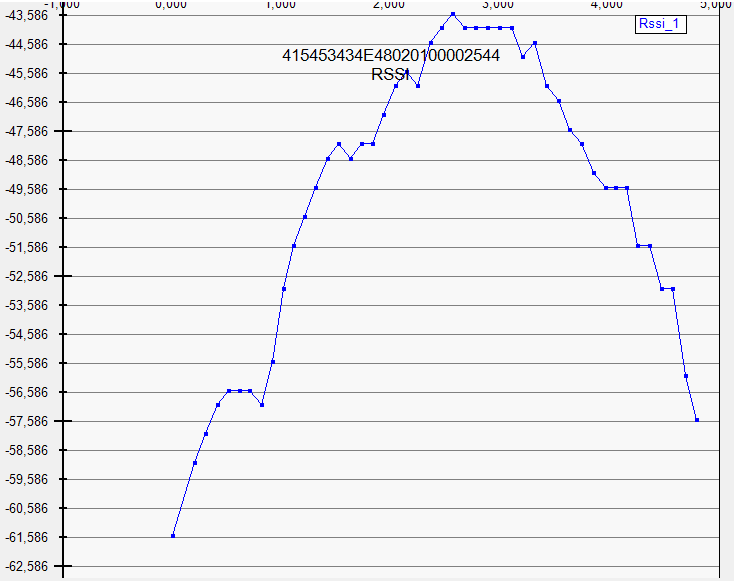
\includegraphics[width=\linewidth]{0_RSSI}
	\captionof{figure}{1 antenne aan deurlijst - Testresultaat}
	\label{fig:ond-rfid-static-0-res}
\end{minipage}

\subsubsection{Deelconclusie}
Uit deze test is duidelijk dat een voorbijkomende tag, bij uitbreiding een getagd asset die de locatie binnenkomt, correct geregistreerd zal worden door het systeem. De hypothese is dus bevestigd. Buiten deze simpele registratietest is er ook nood aan het testen van de invloed van tag oriëntatie en afstand tegenover de antenne. Deze fenomenen worden echter ook onderzocht in de volgende opstelling en zijn hier dus niet apart onderzocht. De beschouwingen en conclusies van test 1 en 2 in de opstelling met 2 antennes zijn dus ook toepasselijk op deze opstelling, uiteraard vereenvoudigd naar 1 antenne.

\subsection{2 antennes aan deurlijst}
\subsubsection{Deelhypothese}
Deze opstelling kan het voorbijkomen en de richting van een getagd asset waarnemen, genomen dat de afstand tussen de tag en de antenne voldoende klein is.

\subsubsection{Test 1: Oriëntatie van de tag}
In deze eerste test wordt de invloed van de oriëntatie van de tag tegenover de antennes bepaald, aangezien deze oriëntatie in theorie een invloed heeft op de gemeten RSSI waarde. De opstelling voor deze test is als volgt: 2 antennes zijn in een deuropening geplaatst, naast elkaar. Bij het binnenkomen wordt eerst antenne 1, en daarna antenne 2 gepasseerd. Er worden 4 oriëntaties onderzocht, nl. horizontaal (a) en verticaal (b) in een evenwijdig vlak aan de antennes, en horizontaal (c) en verticaal (d) loodrecht op het vlak van de antennes. Voor elk van deze deeltesten geld een afstand tussen de tag en de antenne van ~30cm. Bij elk scenario is zowel de richting in als uit getest, echter zullen deze resultaten enkel beide worden getoond als er een meerwaarde is.
In theorie zouden a en b ruwweg dezelfde resultaten moeten geven, terwijl c en d een lagere RSSI zouden moeten geven. Echter zou het in elk geval detecteerbaar moeten zijn.

\paragraph{a) Horizontaal in antennevlak}
\begin{minipage}{0.55\textwidth}
Uit bijhorende grafiek, die de tag toont die uit de locatie ging, is duidelijk een opeenvolging van pieken te zien. Dit met volgorde 2 (groen) -> 1 (blauw), wat inderdaad uit de locatie gaan is. Deze detectie is dus geslaagd. De piekhoogte is niet gelijk, ondanks dat de antennes hetzelfde type zijn. Dit is kalibreerbaar maar zoals zichtbaar is dit niet nodig voor een toepassing als deze.
\end{minipage}
\hfill
\begin{minipage}{0.42\textwidth}
	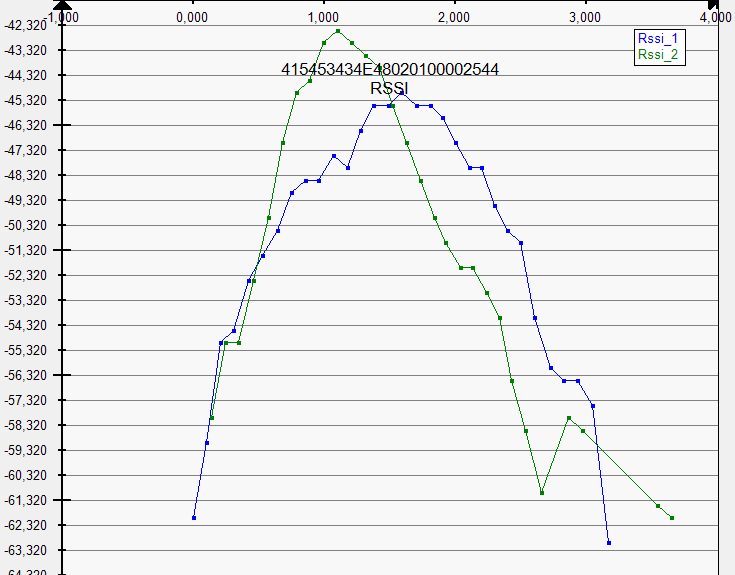
\includegraphics[width=\linewidth]{1a_uit_RSSI}
	\captionof{figure}{2 antennes aan deurlijst - Testresultaat 1a}
	\label{fig:ond-rfid-static-1a-res}
\end{minipage}

\paragraph{b) Verticaal in antennevlak}
\begin{minipage}{0.55\textwidth}
In deze grafiek is vrij gelijkaardig aan de vorige, wat theoretisch ook zou moeten. Er zijn duidelijk 2 pieken zichtbaar, in de juiste volgorde volgend de tag die uit de locatie gaat. Ook is de RSSI gelijkaardig (rond de -40 à -45 dBm).
\end{minipage}
\hfill
\begin{minipage}{0.42\textwidth}
	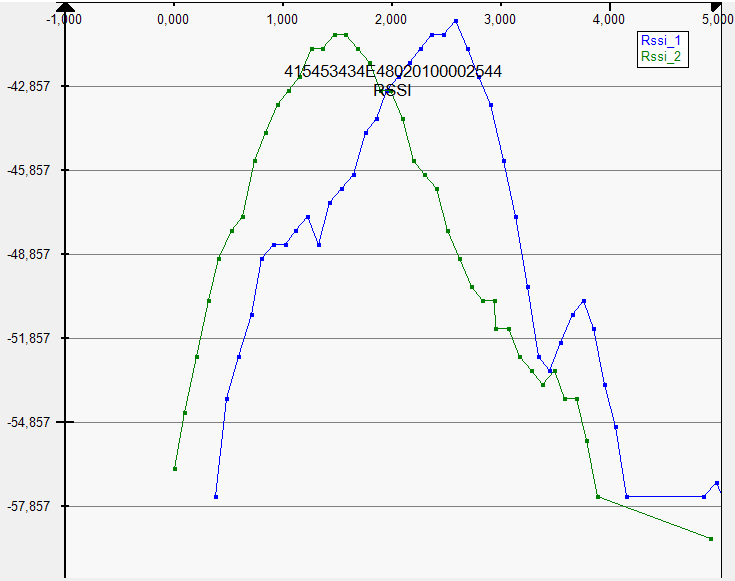
\includegraphics[width=\linewidth]{1b_uit_RSSI}
	\captionof{figure}{2 antennes aan deurlijst - Testresultaat 1b}
	\label{fig:ond-rfid-static-1b-res}
\end{minipage}

\paragraph{c) Horizontaal loodrecht op antennevlak}
\begin{minipage}{0.55\textwidth}
In deze grafiek is een beweging van de tag naar in de locatie weergegeven, hoewel de toppen duidelijk zichtbaar zijn, en in de correcte richting staan, is de top minder duidelijk afgelijnd en meer uitgerokken. Ditzelfde fenomeen is ook zichtbaar in de uit-richting. Ook liggen de toppen iets lager dan de toppen in de vorige 2 deeltests.
\end{minipage}
\hfill
\begin{minipage}{0.42\textwidth}
	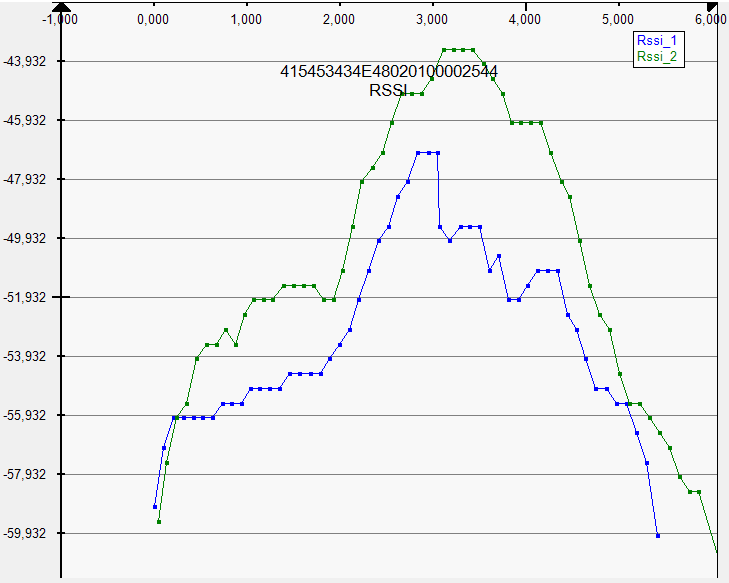
\includegraphics[width=\linewidth]{1c_in_RSSI}
	\captionof{figure}{2 antennes aan deurlijst - Testresultaat 1c}
	\label{fig:ond-rfid-static-1c-res}
\end{minipage}

\paragraph{d) Verticaal loodrecht op antennevlak}
\begin{minipage}{0.55\textwidth}
In deze grafiek in ook een beweging van de tag naar in de locatie weergegeven, en is het fenomeen van meer uitgerokken toppen nog beter zichtbaar. De uit richting vertoont wederom hetzelfde patroon. Deze deeltest ligt dus in lijn met de vorige, maar nog opvallender.
\end{minipage}
\hfill
\begin{minipage}{0.42\textwidth}
	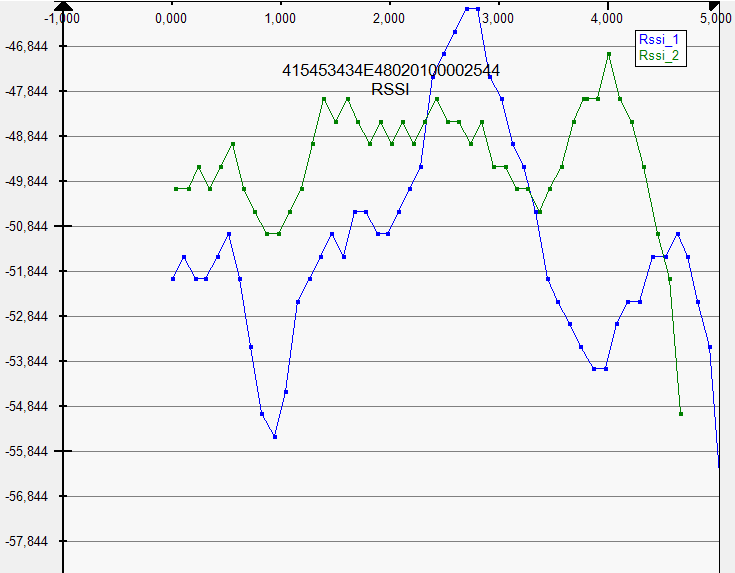
\includegraphics[width=\linewidth]{1d_in_RSSI}
	\captionof{figure}{2 antennes aan deurlijst - Testresultaat 1d}
	\label{fig:ond-rfid-static-1d-res}
\end{minipage}

\paragraph{Testconclusie}
Zoals verwacht is de detectie van de tag en de richting ervan goed zichtbaar en in elk geval correct gemeten. Ook is de meetkwaliteit minder als de tags niet in het vlak van de antenne liggen, daarom lijkt het aanbevolen dit zo veel mogelijk te vermijden.

\subsubsection{Test 2: Afstand tussen tag en antennes}
In deze test wordt de invloed van de afstand tussen de tag en de antennes gemeten, in theorie zou de RSSI van de piek lager moeten zijn als de tag verder van de antenne voorbij komt, en door de conische vorm van het meetveld van de vlakke antenne zouden de pieken meer moeten overlappen. De testopstelling is idem aan Test 1, de oriëntatie van de tag is constant gehouden op horizontaal in hetzelfde vlak als de antennes, en de richting is uit de locatie. De gemeten afstanden zijn 5cm afstand (zeer dicht) en 100cm afstand (zeer ver). Dit kan vergeleken worden met de resultaten van Test 1a, aangezien dit dezelfde opstelling betreft, op 30 cm afstand.

\paragraph{a) 5cm}
\begin{minipage}{0.55\textwidth}
Op deze grafiek is het verwachte resultaat te zien, 2 duidelijke pieken die licht verder uit elkaar liggen, en een hogere RSSI waarde hebben.
\end{minipage}
\hfill
\begin{minipage}{0.42\textwidth}
	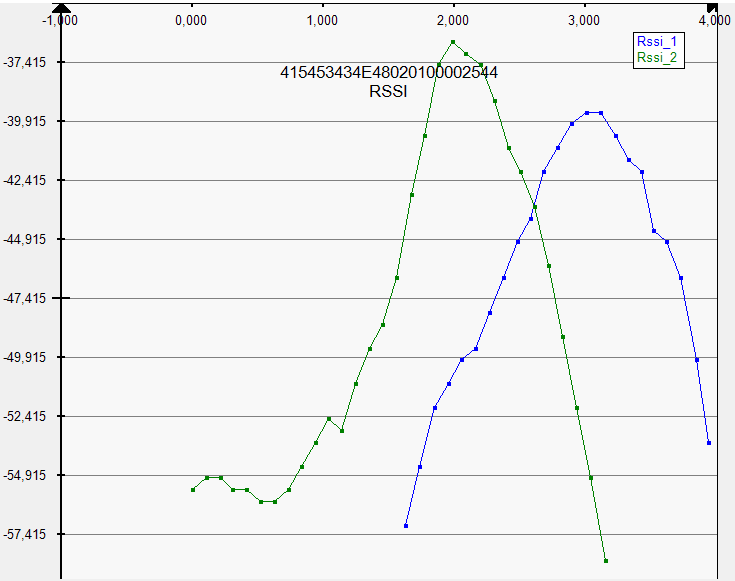
\includegraphics[width=\linewidth]{2a_RSSI}
	\captionof{figure}{2 antennes aan deurlijst - Testresultaat 2a}
	\label{fig:ond-rfid-static-2a-res}
\end{minipage}

\paragraph{b) 100cm}
\begin{minipage}{0.55\textwidth}
Deze grafiek is interessanter dan de vorige, het vermoeden dat de piek minder duidelijk ging zijn en ging overlappen is bevestigd. Uit deze meting kan niet meer afgeleid worden in welke richting de tag voorbij de antennes komt. Ook ligt de RSSI waarde beduidend lager.
\end{minipage}
\hfill
\begin{minipage}{0.42\textwidth}
	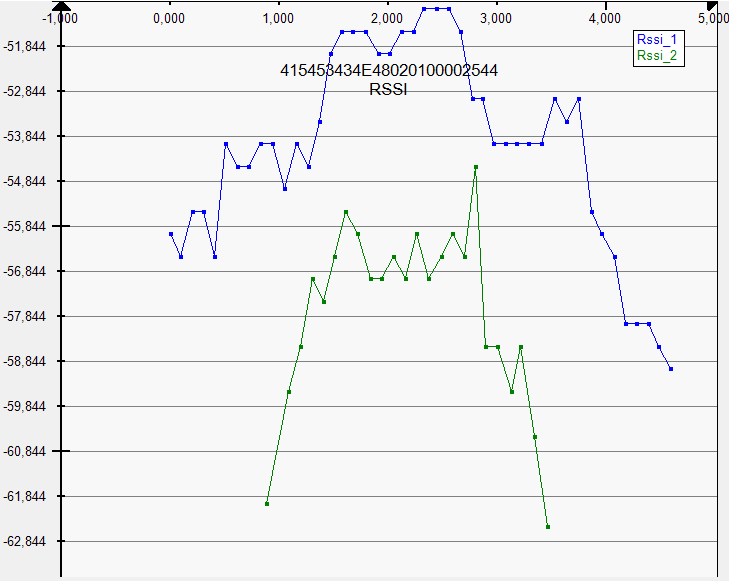
\includegraphics[width=\linewidth]{2b_RSSI}
	\captionof{figure}{2 antennes aan deurlijst - Testresultaat 2b}
	\label{fig:ond-rfid-static-2b-res}
\end{minipage}

\paragraph{Testconclusie}
Zoals werd vermoed is er een bepaalde restrictie op de afstand waarmee de tag de antennes kan voorbijkomen om een goede richtingsdetectie te hebben. 

\subsubsection{Test 3: Afstand tussen de 2 antennes}
Aangezien de reden van de overlappende pieken in vorige test het feit is dat het conische bereik van de 2 antennes elkaar te veel overlapt, is het logisch dat dit effect zal verminderen als deze 2 antennes verder van elkaar geplaatst worden, dit zal getest worden in deze 3e test. De opstelling is identiek aan de test 2, het enige verschil is dat de 2 antennes 20cm uit elkaar gezet zijn.

\paragraph{a) 5cm}
\begin{minipage}{0.55\textwidth}
Dit testresultaat toont wederom 2 mooie pieken, deze keer iets verder uit elkaar liggend door de afstand tussen de antennes, en dit met een lage RSSI waarde.
\end{minipage}
\hfill
\begin{minipage}{0.42\textwidth}
	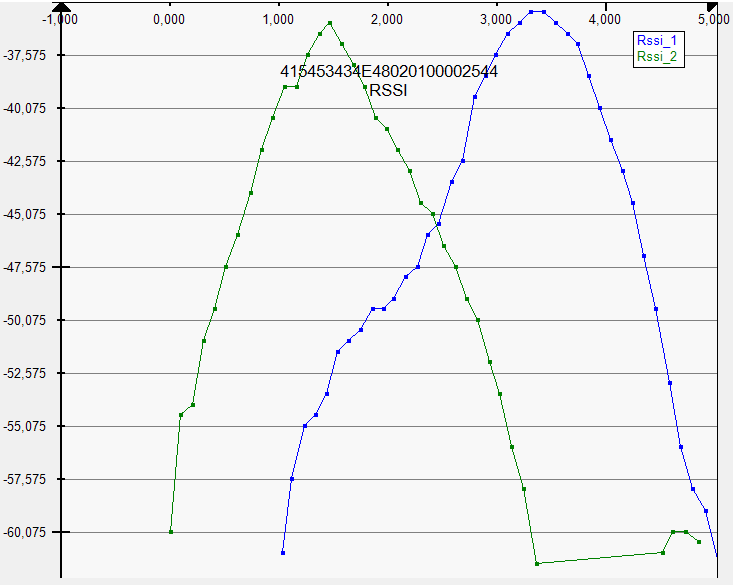
\includegraphics[width=\linewidth]{3a_RSSI}
	\captionof{figure}{2 antennes aan deurlijst - Testresultaat 3a}
	\label{fig:ond-rfid-static-3a-res}
\end{minipage}

\paragraph{b) 30cm}
\begin{minipage}{0.55\textwidth}
Hier zien we ongeveer hetzelfde als op de vorige grafiek, enkel licht meer uitgerokken en met een lagere RSSI waarde.
\end{minipage}
\hfill
\begin{minipage}{0.42\textwidth}
	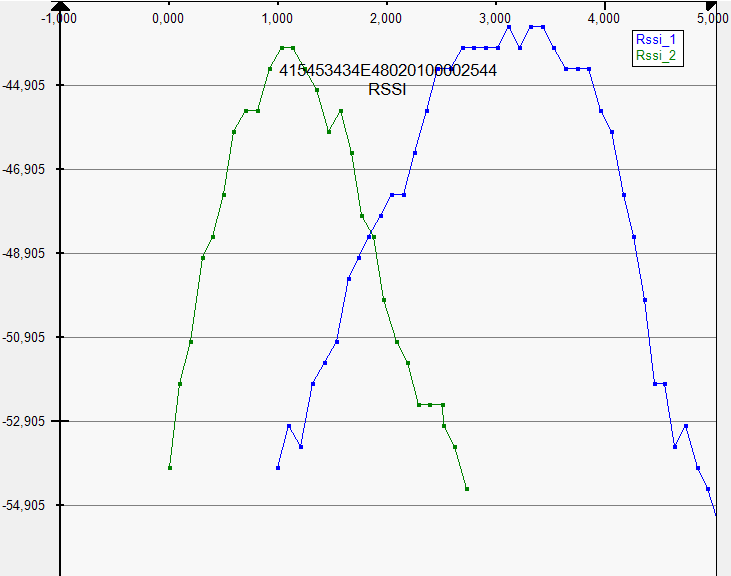
\includegraphics[width=\linewidth]{3b_RSSI}
	\captionof{figure}{2 antennes aan deurlijst - Testresultaat 3b}
	\label{fig:ond-rfid-static-3b-res}
\end{minipage}

\paragraph{c) 100cm}
\begin{minipage}{0.55\textwidth}
Dit resultaat is het voornaamste van deze test, we zien, zoals bij test 2, dat de pieken weer hard zijn uitgerokken, maar door de extra afstand tussen de antennes is de volgorde wel weer zichtbaar.
\end{minipage}
\hfill
\begin{minipage}{0.42\textwidth}
	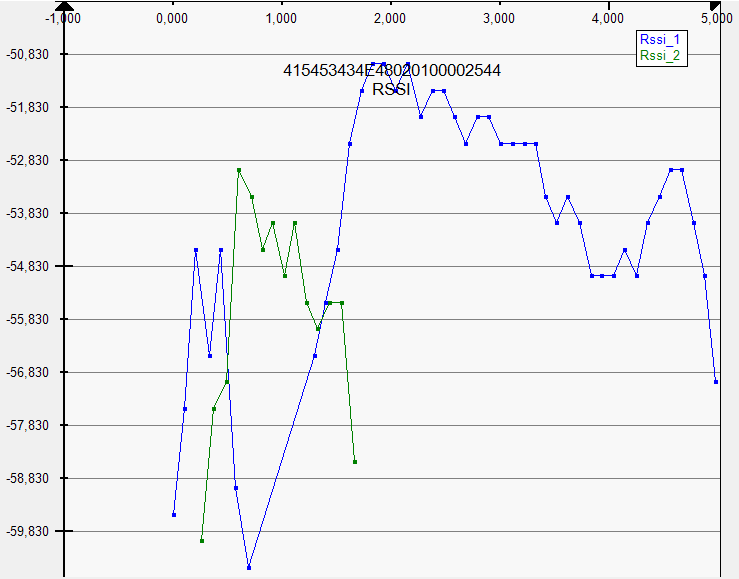
\includegraphics[width=\linewidth]{3c_RSSI}
	\captionof{figure}{2 antennes aan deurlijst - Testresultaat 3c}
	\label{fig:ond-rfid-static-3c-res}
\end{minipage}

\paragraph{Testconclusie}
Het blijkt inderdaad correct dat het verder uit elkaar plaatsen van de antennes een positief effect heeft op het uit elkaar trekken van de pieken in de RSSI curve, wat nodig is naarmate de tag verder van de antenne voorbij komt.

\subsubsection{Deelconclusie}
Deze opstelling slaagt er inderdaad in om een voorbijkomende tag en zijn richting te registreren, mits de afstand beperkt is, de hypothese is dus correct. Er kan echter wel aan toegevoegd worden dat, als de afstand niet meer voldoende klein is, dat de afstand tussen de antennes kan vergroot worden. Dit is in een reële situatie echter niet praktisch aangezien een deur meestal een beperkte breedte heeft. Voor een standaard deur zal dit geen probleem zijn aangezien de maximale afstand in een deur ook beperkt is, maar voor bv. een poortdoorgang kan dit wel problemen opleveren. In een gang met een quasi onbeperkte beschikbare breedte is dit wel mogelijk.

\subsection{1 antenne tegenover deur}
\subsubsection{Deelhypothese}
Deze opstelling kan het voorbijkomen en de richting van een getagd asset waarnemen, genomen dat de afstand tussen de antenne en de deur voldoende klein is zodat de antenne de tag kan registreren.

\subsubsection{Test 1: PoC}
Deze eerste test bestaat uit een proof of concept, hierin wordt getest of het op zijn minst mogelijk is om de richting van de bewegende tag te bepalen uit de gemeten data. 
In deze test wordt een antenne geplaatst tegen een muur, met daarvoor een kar met een tag op (horizontaal in het vlak van de antenne). Deze kar zal voor deze test achteruit en vooruit gerold worden. 

\paragraph{Resultaat}
Onderstaande grafieken tonen de verandering in RSSI van beide testen, met het rollen van de kar weg van de antenne links, en naar de antenne toe rechts. In deze grafieken is deze richting zeer mooi zichtbaar, de RSSI verlaagt als de kar wegrolt, en verhoogt als deze naar de antenne toe rolt.

\begin{minipage}{0.42\textwidth}
	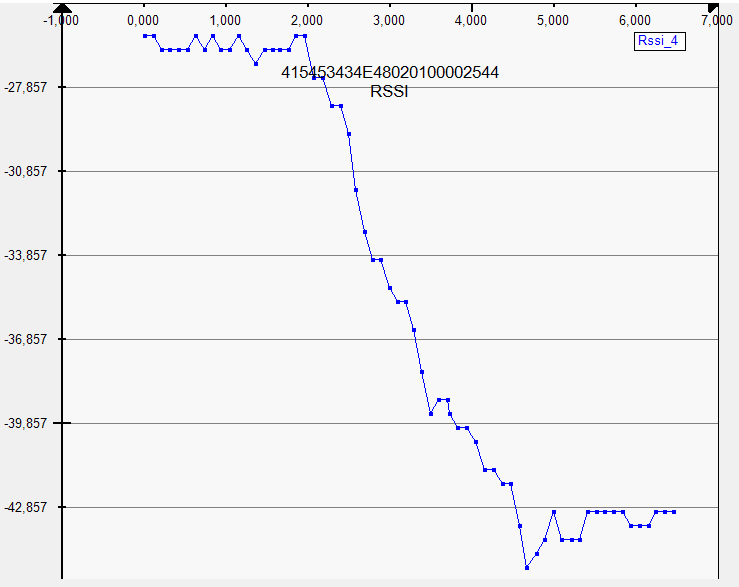
\includegraphics[width=\linewidth]{4c_RSSI}
	\captionof{figure}{1 antenne tegenover deur - Testresultaat 1 uit}
	\label{fig:ond-rfid-static-4c-res}
\end{minipage}
\hfill
\begin{minipage}{0.42\textwidth}
	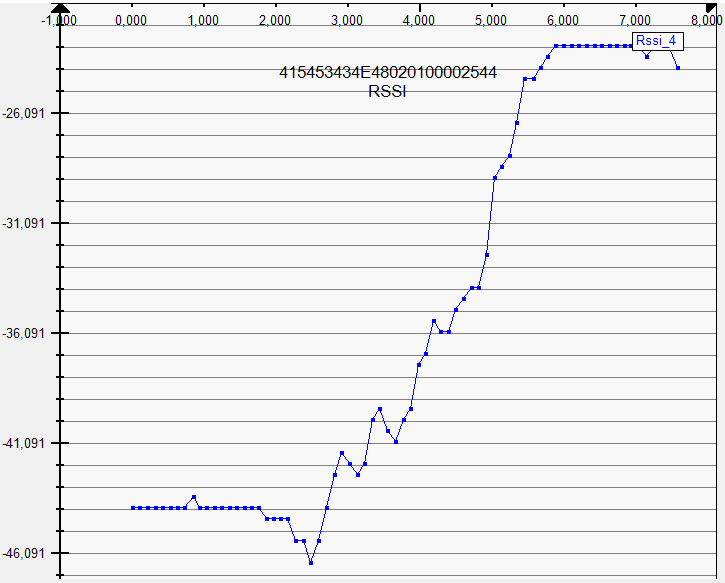
\includegraphics[width=\linewidth]{4d_RSSI}
	\captionof{figure}{1 antenne tegenover deur - Testresultaat 1 in}
	\label{fig:ond-rfid-static-4d-res}
\end{minipage}

\paragraph{Testconclusie}
Uit deze resultaten is zeer mooi te zien dat de richting van de verplaatsing op de lijn voor een antenne duidelijk zichtbaar is.

\subsubsection{Test 2: Variabele afstand tot deur}
In deze test wordt de opstelling realistischer gemaakt, de antenne wordt op respectievelijk 100 en 200 cm afstand van de deur geplaatst, en er wordt met de kar met bevestigde RFID tag van test 1 door de deur gereden, zowel in als uit de kamer, direct de hoek om. 

\paragraph{a) 100cm}
Hieronder is het binnenkomen (links) en het verlaten (rechts) van de locatie te zien, zoals duidelijk te zien is is de grafiek zeer veel minder duidelijk dan in de ideale situatie van test 1. Vermoedelijk is de 'staart' die niet in de meting past (rechts aanhangsel bij inwaarts en links bij uitwaarts) het gevolg van het feit dat de kar op dat moment 90° gedraaid in de kamer aanwezig is, resp. na en voor de draaibeweging door de deur. Op dit moment bevind de tag zich in het leesveld van de antenne, maar niet meer in hetzelfde vlak. Deze onderlinge oriëntatie zorgt voor een slechte RSSI waarde, zoals aangetoond tijdens test 1 van de vorige opstelling. Voor de duidelijkheid van de 'uit' meting is dit niet zo zeer een probleem, maar wel voor de 'in' meting.

\begin{minipage}{0.42\textwidth}
	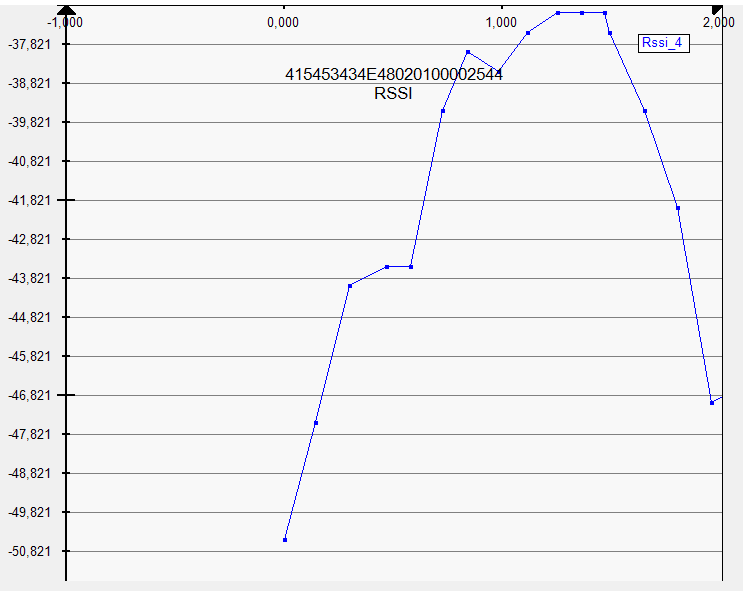
\includegraphics[width=\linewidth]{5a_in_RSSI}
	\captionof{figure}{1 antenne tegenover deur - Testresultaat 2a in}
	\label{fig:ond-rfid-static-5ain-res}
\end{minipage}
\hfill
\begin{minipage}{0.42\textwidth}
	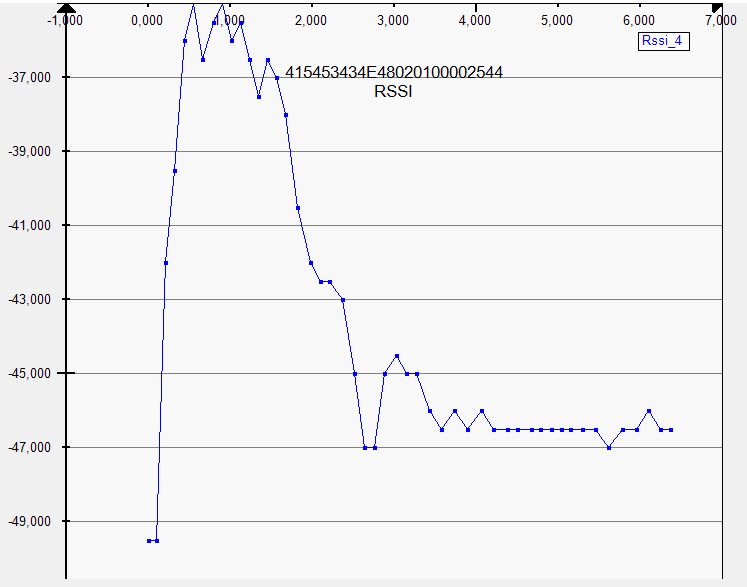
\includegraphics[width=\linewidth]{5a_uit_RSSI}
	\captionof{figure}{1 antenne tegenover deur - Testresultaat 2a uit}
	\label{fig:ond-rfid-static-5auit-res}
\end{minipage}

\paragraph{b) 200cm}
Hieronder is wederom het binnenkomen (links) en het verlaten (rechts) van de locatie te zien. In dit geval is de onduidelijkheid zichtbaar in vorige deeltest nog extremer zichtbaar. Alhoewel het in theorie de richting nog steeds eenduidig zichtbaar is, is het nog minder duidelijk, en deze onduidelijkheid vergroot naarmate de tussenliggende afstand groter wordt. Ook de RSSI waarde ligt logischerwijs lager.

\begin{minipage}{0.42\textwidth}
	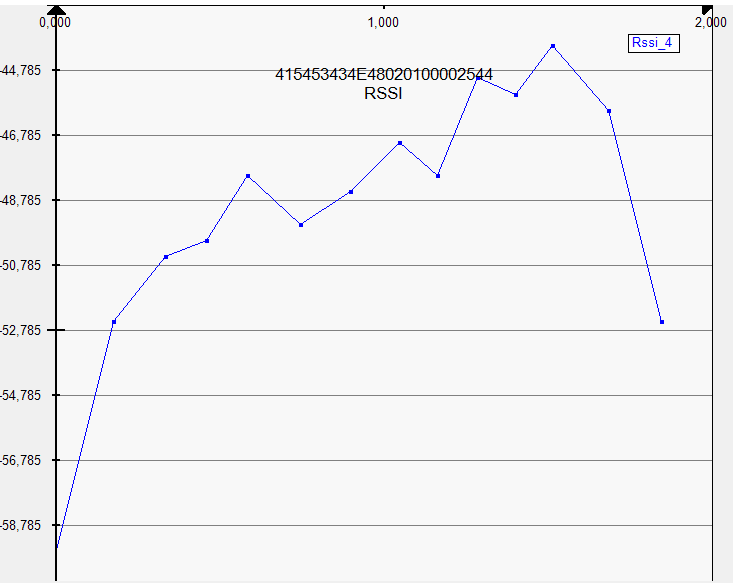
\includegraphics[width=\linewidth]{5b_in_RSSI}
	\captionof{figure}{1 antenne tegenover deur - Testresultaat 2b in}
	\label{fig:ond-rfid-static-5bin-res}
\end{minipage}
\hfill
\begin{minipage}{0.42\textwidth}
	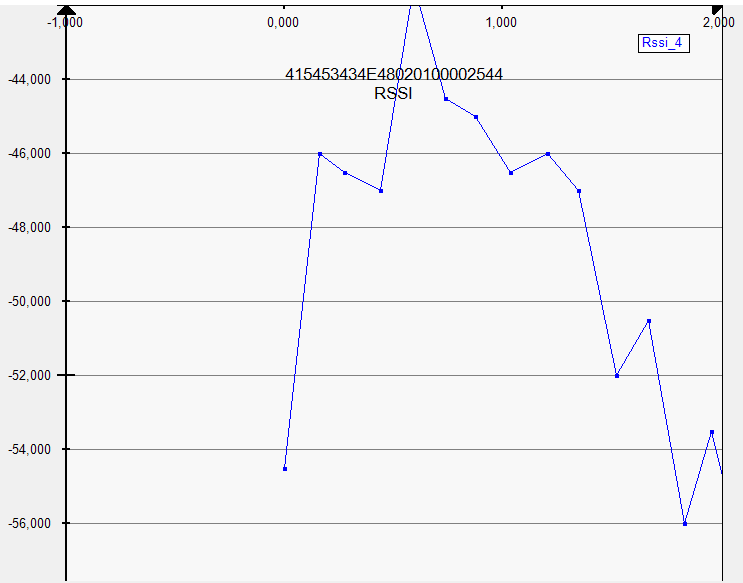
\includegraphics[width=\linewidth]{5b_uit_RSSI}
	\captionof{figure}{1 antenne tegenover deur - Testresultaat 2b uit}
	\label{fig:ond-rfid-static-5buit-res}
\end{minipage}

\paragraph{Testconclusie}
Deze testen tonen aan dat de meting in een realistisch scenario veel minder optimaal is als in het optimaal scenario van test 1 aangezien de meetpunten rond het dichter/verder komen voor onduidelijkheden zorgen die niet eenduidig uit de data te halen zijn.

\subsubsection{Test 3: Langere meetafstand}
Aangezien een simpele draai rond het deurgat te slechte data oplevert om eenduidig de richting te bepalen, kan het een idee zijn om de kar langer op de lijn van de antenne te laten rijden om zo het relatieve aantal van meetpunten voor de richtingsdetectie op te krikken tegenover de meetpunten bij het in- en uit stappen van het meetbereik van de antenne. Dit wordt in volgende test bekeken, hierbij is de opstelling idem aan test 2b, maar zal de kar tot tegen de antenne rijden alvorens af te slaan.

\paragraph{Resultaat}
Onderstaande grafieken tonen wederom de verandering in RSSI van beide richtingen, met het rollen van de kar naar de antenne links, en weg van de antenne rechts. Alhoewel de 'staarten' uit test 2 nog steeds zichtbaar zijn, overheersen ze de grafiek niet meer en dus is deze grafiek veel eenduidiger en kan uit de richting van de scheefheid de richting van verplaatsing worden afgeleid.

\begin{minipage}{0.42\textwidth}
	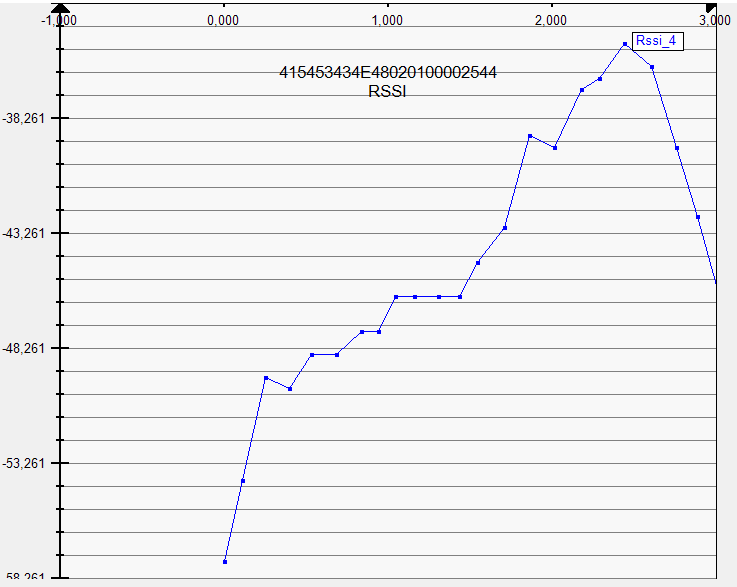
\includegraphics[width=\linewidth]{5c_in_RSSI}
	\captionof{figure}{1 antenne tegenover deur - Testresultaat 3 in}
	\label{fig:ond-rfid-static-5cin-res}
\end{minipage}
\hfill
\begin{minipage}{0.42\textwidth}
	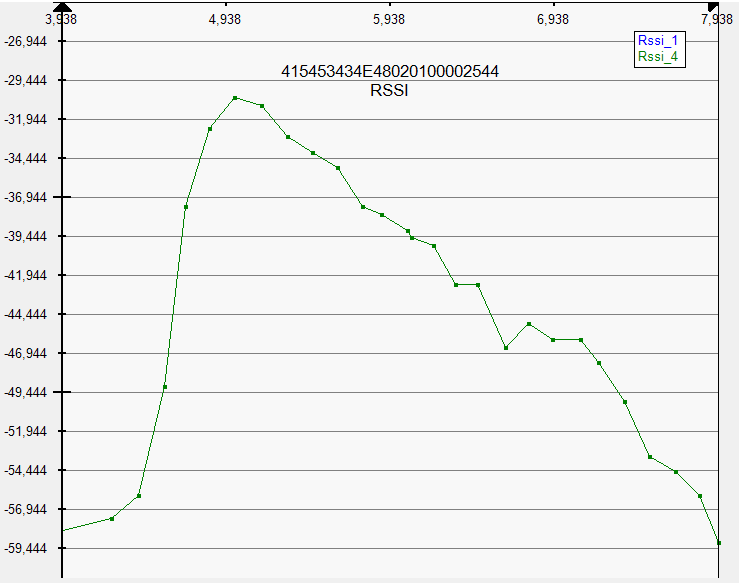
\includegraphics[width=\linewidth]{5c_uit_RSSI}
	\captionof{figure}{1 antenne tegenover deur - Testresultaat 3 uit}
	\label{fig:ond-rfid-static-5cuit-res}
\end{minipage}

\paragraph{Testconclusie}
Het vermoeden dat de resultaten beter zijn als er verder op de lijn voor de antenne wordt gewandeld lijkt te zijn bevestigd met deze test.

\subsubsection{Deelconclusie}
In ideale omstandigheden blijkt dit concept zeer goed te werken, echter zijn er enkele neveneffecten van een realistische draai door een deur die moeten gecompenseerd worden met een langere lengte op de lijn voor de antenne te lopen. De vooropgestelde hypothese is dus niet correct en moet aangevuld worden met deze nieuwe informatie. In praktijk wilt dit zeggen dat dit niet werkt voor een normale deuropening en vorige opstelling dus gebruikt zal moeten worden. Echter kan het wel een oplossing zijn voor een (korte) gang of dergelijke waar de assets sowieso door moeten om een berging of magazijn te bereiken, want vanaf er enige afstand wordt gedaan werkt dit wel zeer goed. 

\subsection{1 tag aan deurlijst}
\subsubsection{Deelhypothese}
Deze opstelling is in staat om verspreide, getagde assets te detecteren en eenduidig een locatie toe te wijzen.

\subsubsection{Test 1: Ideale situatie}
De opstelling voor deze test is als volgt: Een rijdende kar is voorzien van een RFID-reader, of meer bepaald een vlakke antenne, welke opzij (rechts) is gericht. Verder is er een een locatie, bestaande uit 1 ommuurde ruimte, deze is voorzien van 1 locatie tag (Tagcode 4) aan het deurframe, langs de rechterkant (zodat de antenne op de kar de tag kan lezen bij het binnenkomen). Vervolgens bevinden zich verspreid over deze ruimte 4 assets (Tagcode 1, 2, 3 en 5), getagd met een asset tag. Als laatste is er aan de deurlijst aan de linker kant ook een locatie tag (Tagcode 6) aangebracht, voor een andere locatie dan deze. In en opstelling in productie zou deze aan de deur van een nieuwe locatie hangen, maar in deze opstelling is zijn functie louter om aan te geven wanneer de locatie wordt verlaten. Alle tags (zowel locatie als asset) bevinden zich op dezelfde hoogte als de antenne op de kar. De test is geslaagd als alle asset tags gemeten worden tussen het meten van eerst de locatie tag van de locatie zelf eenderzijds en, en de tag van de andere locatie anderzijds.

\paragraph{Resultaat}
De resultaten van deze test zijn ondergebracht in grafiek~\ref{fig:ond-rfid-dynamic-6a-res}. Met leesbaarheid in gedachten zijn de tijdsspannes tussen de registraties van de tags weggelaten uit de grafiek, in praktijk liggen deze verder uit elkaar in de tijd maar de volgorde is hier voornamelijk van belang. We kunnen zeer duidelijk zien dat deze test geslaagd is, we registreren eerst tag 4, welke duidelijk maakt dat we ons vanaf hier binnen de locatie bevinden. Elke asset tag die tussen dit moment, en het moment dat een andere locatie tag wordt gedetecteerd, ligt in deze locatie. De 2e locatie tag is de laatste die we detecteren dus er is correct bepaald dat alle assets zich in deze locatie bevinden. Wel zien we een groot verschil in aantal meetpunten, tag 5 wordt zo maar 2x gedetecteerd, in vergelijking tot de meer dan 50 meetpunten voor tag 3. Dit is echter niet geheel verrassend, aangezien het asset met tag 5 veel dieper in de kamer lag dan asset 3.

\begin{figure}[h]
	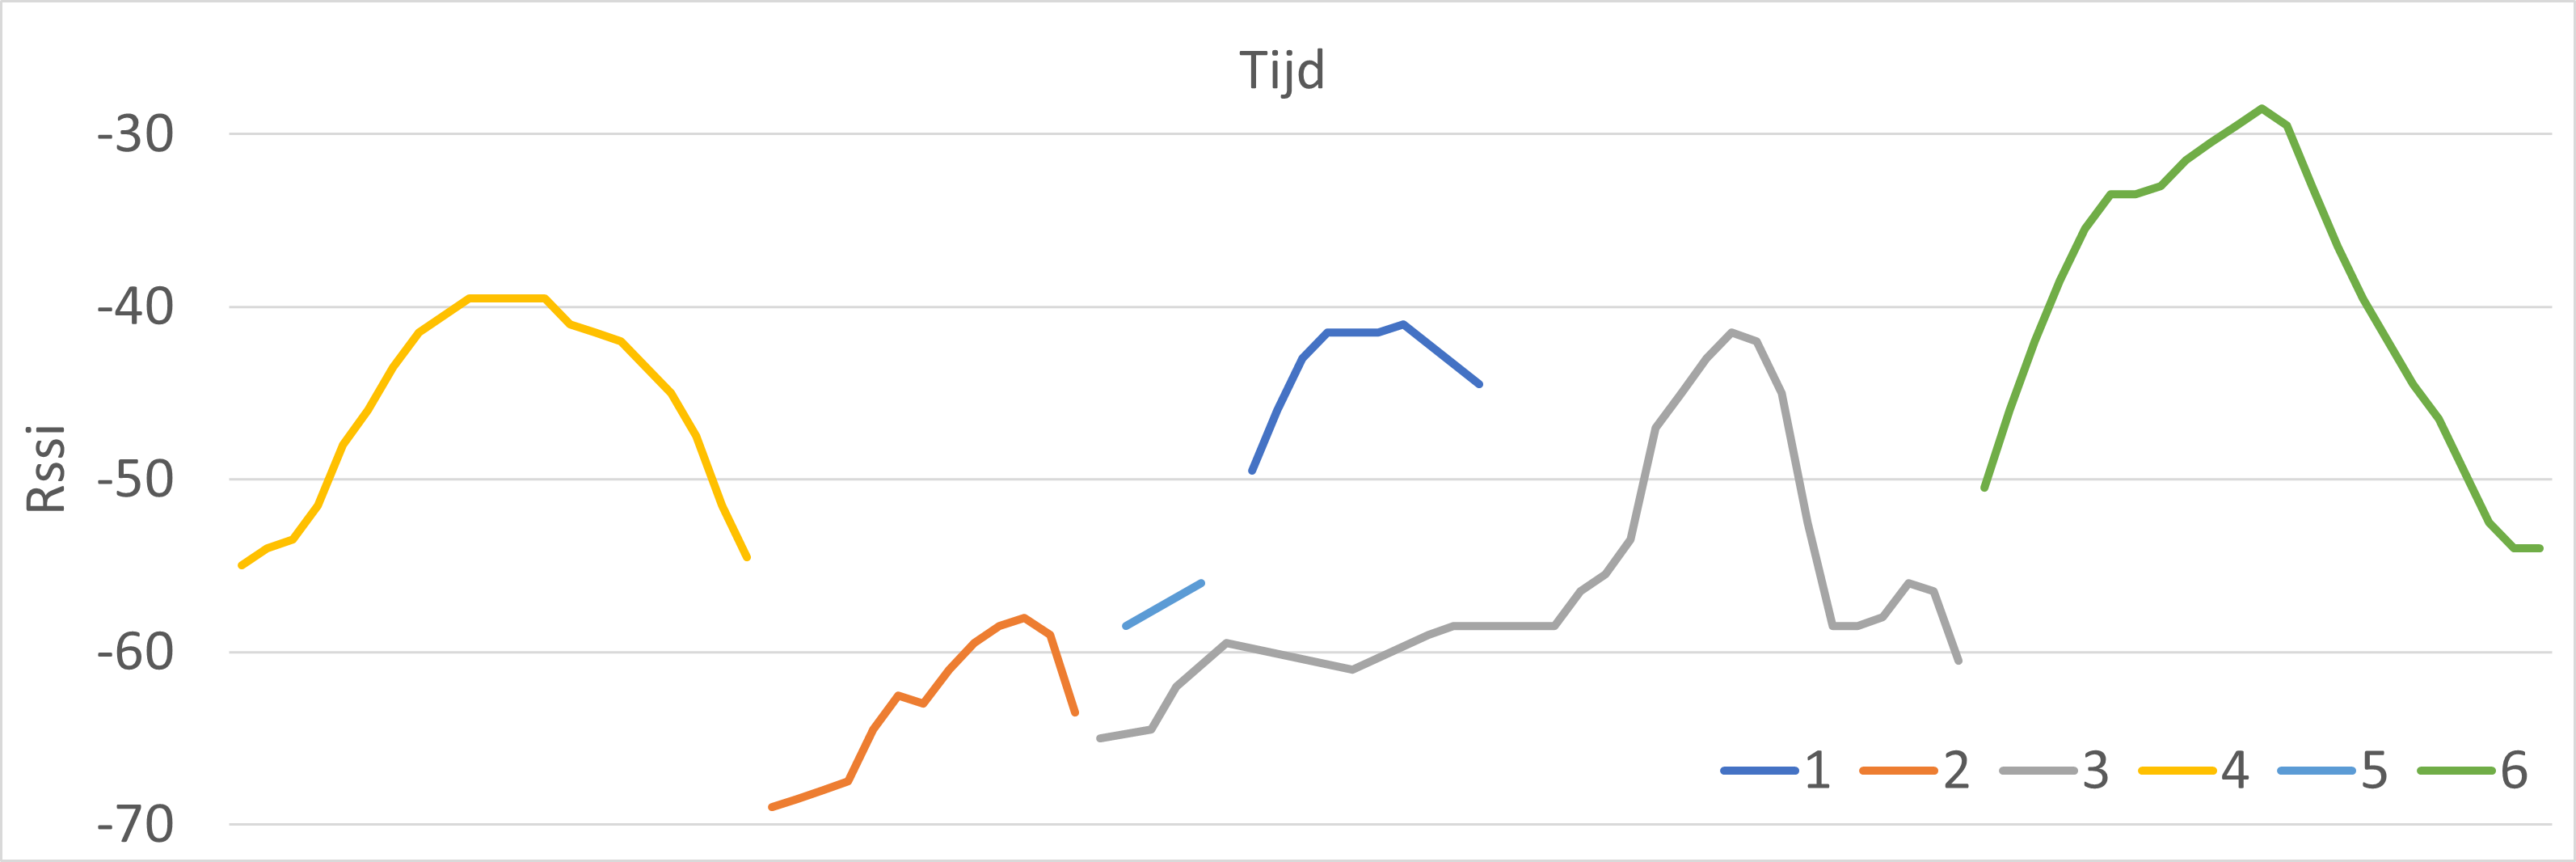
\includegraphics[width=\linewidth]{6a_RSSI}
	\caption{1 tag aan deurlijst - Testresultaat 1}
	\label{fig:ond-rfid-dynamic-6a-res}
\end{figure}

\paragraph{Testconclusie}
Het doel van de test, namelijk het detecteren van alle assets en ze correct plaatsen in de locatie is geslaagd. Het feit dat er een groot verschil bestaat in het aantal meet- of detectiepunten wekt wel het vermoeden dat het voornaamste probleem met dit scenario zal liggen in het detecteren van alle aanwezige assets, en niet zo zeer in het bekomen van een correcte lokalisatie.

\subsubsection{Test 2: Realistische situatie}
In tegenstelling tot vorige situatie is het natuurlijk geen gegeven dat alle asset tags zich ook op ruwweg dezelfde hoogte als de antenne zullen bevinden aangezien assets zelf zich in theorie overal in de kamer kunnen bevinden, inclusief op tafels of kasten. Deze test zal dus dezelfde opstelling nemen als de vorige test, maar de assets zullen zich ook op verschillende hoogtes bevinden.

\paragraph{Resultaat}
Dit resultaat toont de vrees van vorige test aan, de detectie is helaas veel slechter als de tags niet op het niveau van de antenne liggen. De volgorde is nog steeds correct, dus qua lokalisatie is er geen probleem. Echter is bij elke asset tag het aantal meet- of detectiepunten afgenomen en is de RSSI gezakt. Tag 5 is zelfs volledig verdwenen uit de data en is dus niet gedetecteerd.
\begin{figure}[h]
	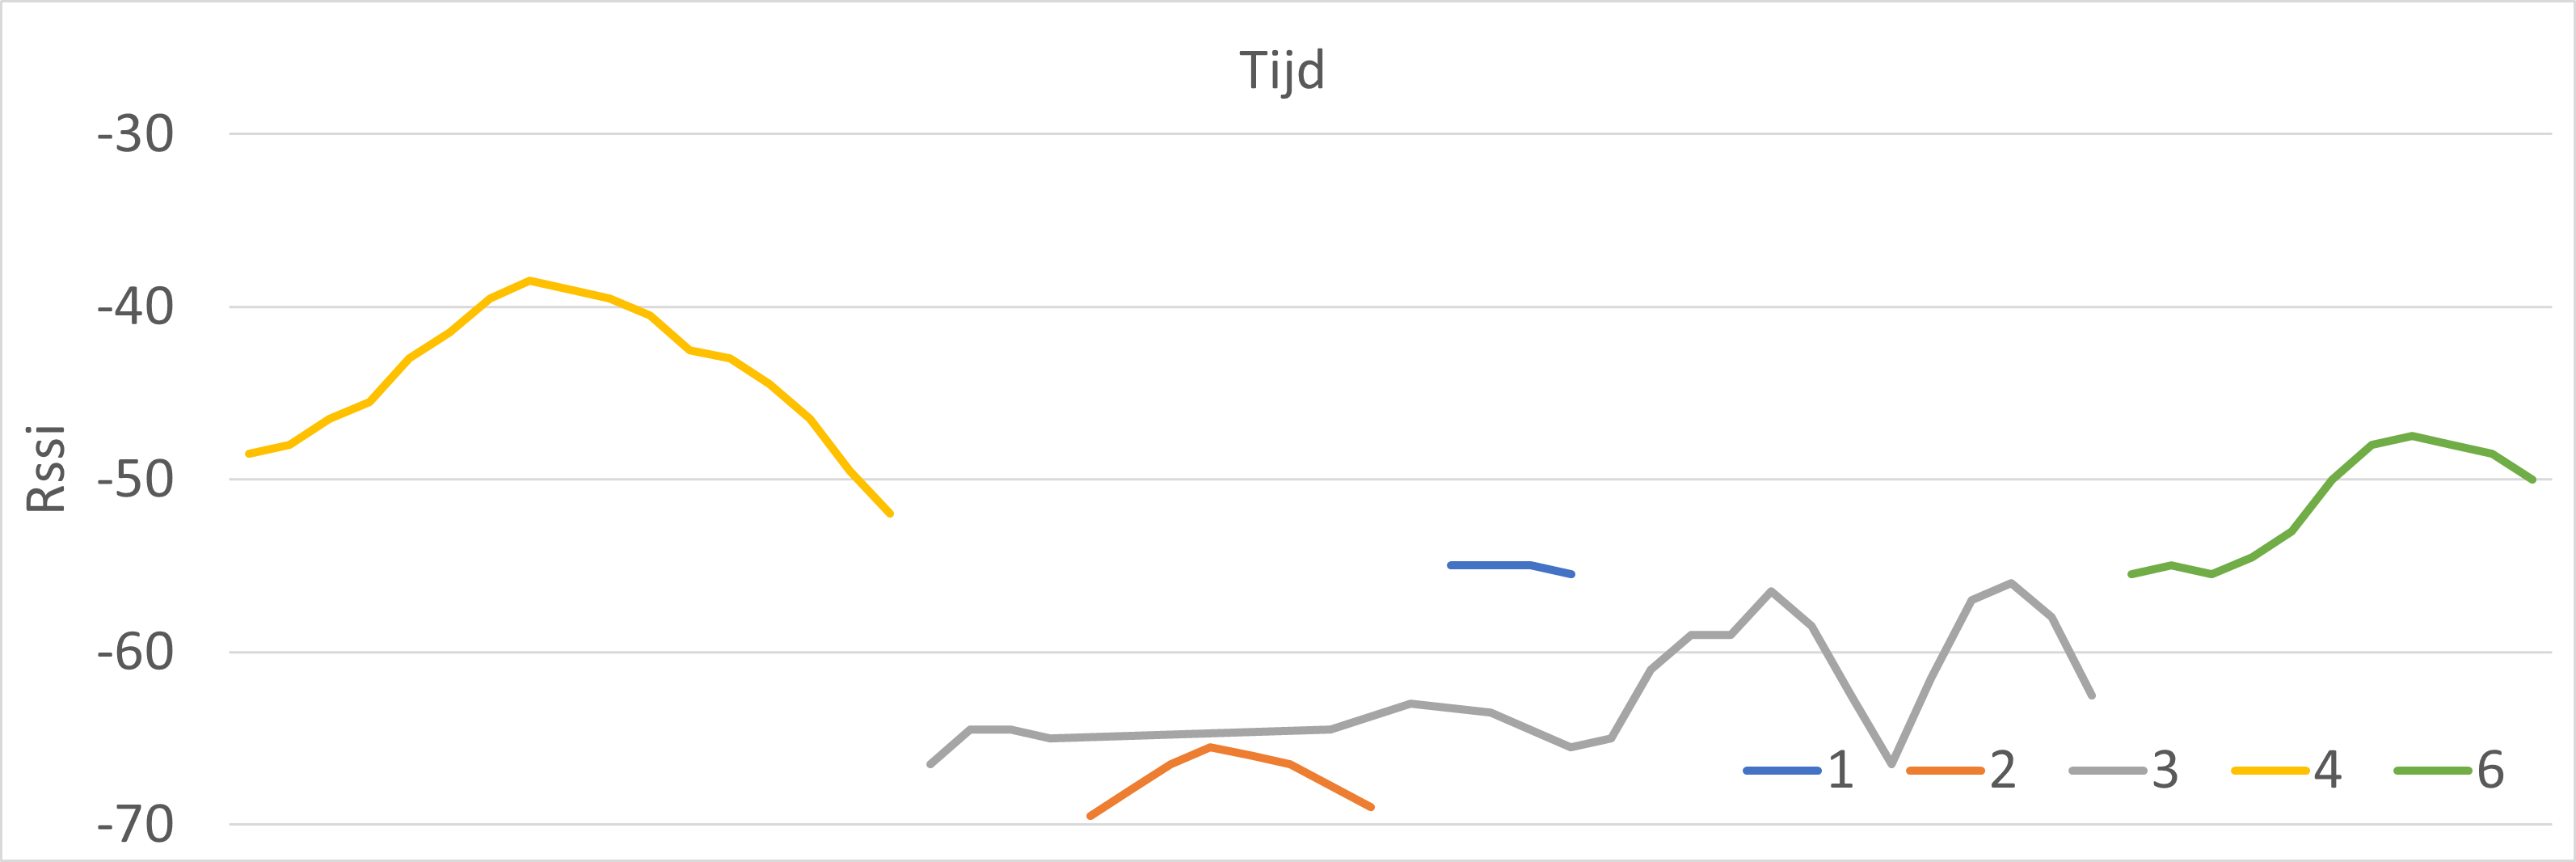
\includegraphics[width=\linewidth]{6b_RSSI}
	\caption{1 tag aan deurlijst - Testresultaat 2}
	\label{fig:ond-rfid-dynamic-6b-res}
\end{figure}

\paragraph{Testconclusie}
Als de asset tags niet meer op hetzelfde niveau liggen als de antenne, is hun detectie dus veel minder. Dit hoeft echter niet zo'n zeer probleem te zijn aangezien 1 meetpunt in theorie voldoende is om te weten dat het asset aanwezig is, een tag die niet aanwezig is op de locatie zal uiteraard ook niet 1x antwoorden. Wel is het wegvallen van tags een probleem, want dan kan bijhorend asset niet gelokaliseerd worden, en deze kans wordt groter als de detectie verslecht.

\subsubsection{Deelconclusie}
Qua lokalisatie blijkt dit concept perfect te werken, echter is dit logisch gezien ook niet verrassend. Het voornaamste probleem is het kunnen detecteren van alle aanwezige tags, wat met een RFID opstelling niet vanzelfsprekend is. Uiteraard is het mogelijk om met een andere hardwareopstelling, bv. antennes op verschillende hoogtes, of een staafantenne met een ander bereikveld dan een vlakke antenne, mogelijk om betere detectie te bekomen. Echter evolueert dit op deze manier in een RFID detectieprobleem en komt daarmee buiten de scope, nl. lokalisatie, van dit onderzoek te liggen. Verder is er binnen Aucxis voldoende ervaring op dit veld dat verder onderzoek nutteloos zou zijn.

\section{BLE Vooronderzoek}
Voordat overgegaan kan worden naar het onderzoeken van de opstellingen die gebruik maken van BLE, is het nodig enkele testen te doen om het gedrag van BLE vast te stellen, en om enkele veronderstellingen te testen.

\subsubsection{Test 1: Variatietest}
Aangezien de lokalisatieopstellingen verder in dit hoofdstuk gebruik zullen maken van RSSI waardes om de locatie van de beacons, en dus ook de bijhorende assets, te bepalen, is het belangrijk dat deze waardes constant zijn in de tijd als alle andere variabelen constant zijn. 
Voor deze test worden de gateway en de beacon op een afstand van 150cm uit elkaar gelegd, in hetzelfde vlak. Vervolgens wordt over lange tijd de RSSI waardes gemeten. Dit experiment wordt uitgevoerd bij 3 en bij 30 beaconberichten per gatewaybericht, dit om te bekijken of dit een effect heeft. Want logischerwijs zal ook deze verhouding een invloed hebben, nl. hoe meer berichten de gateway heeft ontvangen, hoe meer de eventuele extreme waarden zullen uitgemiddeld worden en hoe stabieler de waarden uitgestuurd door de gateway zullen worden.
Beide experimenten zijn uitgevoerd met 5 verschillende beacons van het type MokoSmart H5, en 2 beacons van het type MokoSmart M2. Ze zijn allen aangeduid a.d.h.v. de laatste 2 karakters van hun MAC adres.

\paragraph{a) 3 beaconberichten per gatewaybericht}
Uit dit testresultaat is duidelijk af te lijden dat een uitmiddeling van 3 berichten een zeer grote variatie veroorzaakt in de RSSI waarden, met bij bv. beacon FB een verschil tussen de uitersten van 14 dBm. Aangezien de FSPL formule duidelijk maakt dat in theorie een verschil van 6 dBm een verdubbeling van de afstand betekend, komt deze onzekerheid neer op een afstandsverschil van ongeveer factor 4, het spreekt voor zich dat dit nefast is voor elke poging tot lokalisatie.

\begin{figure}[h]
	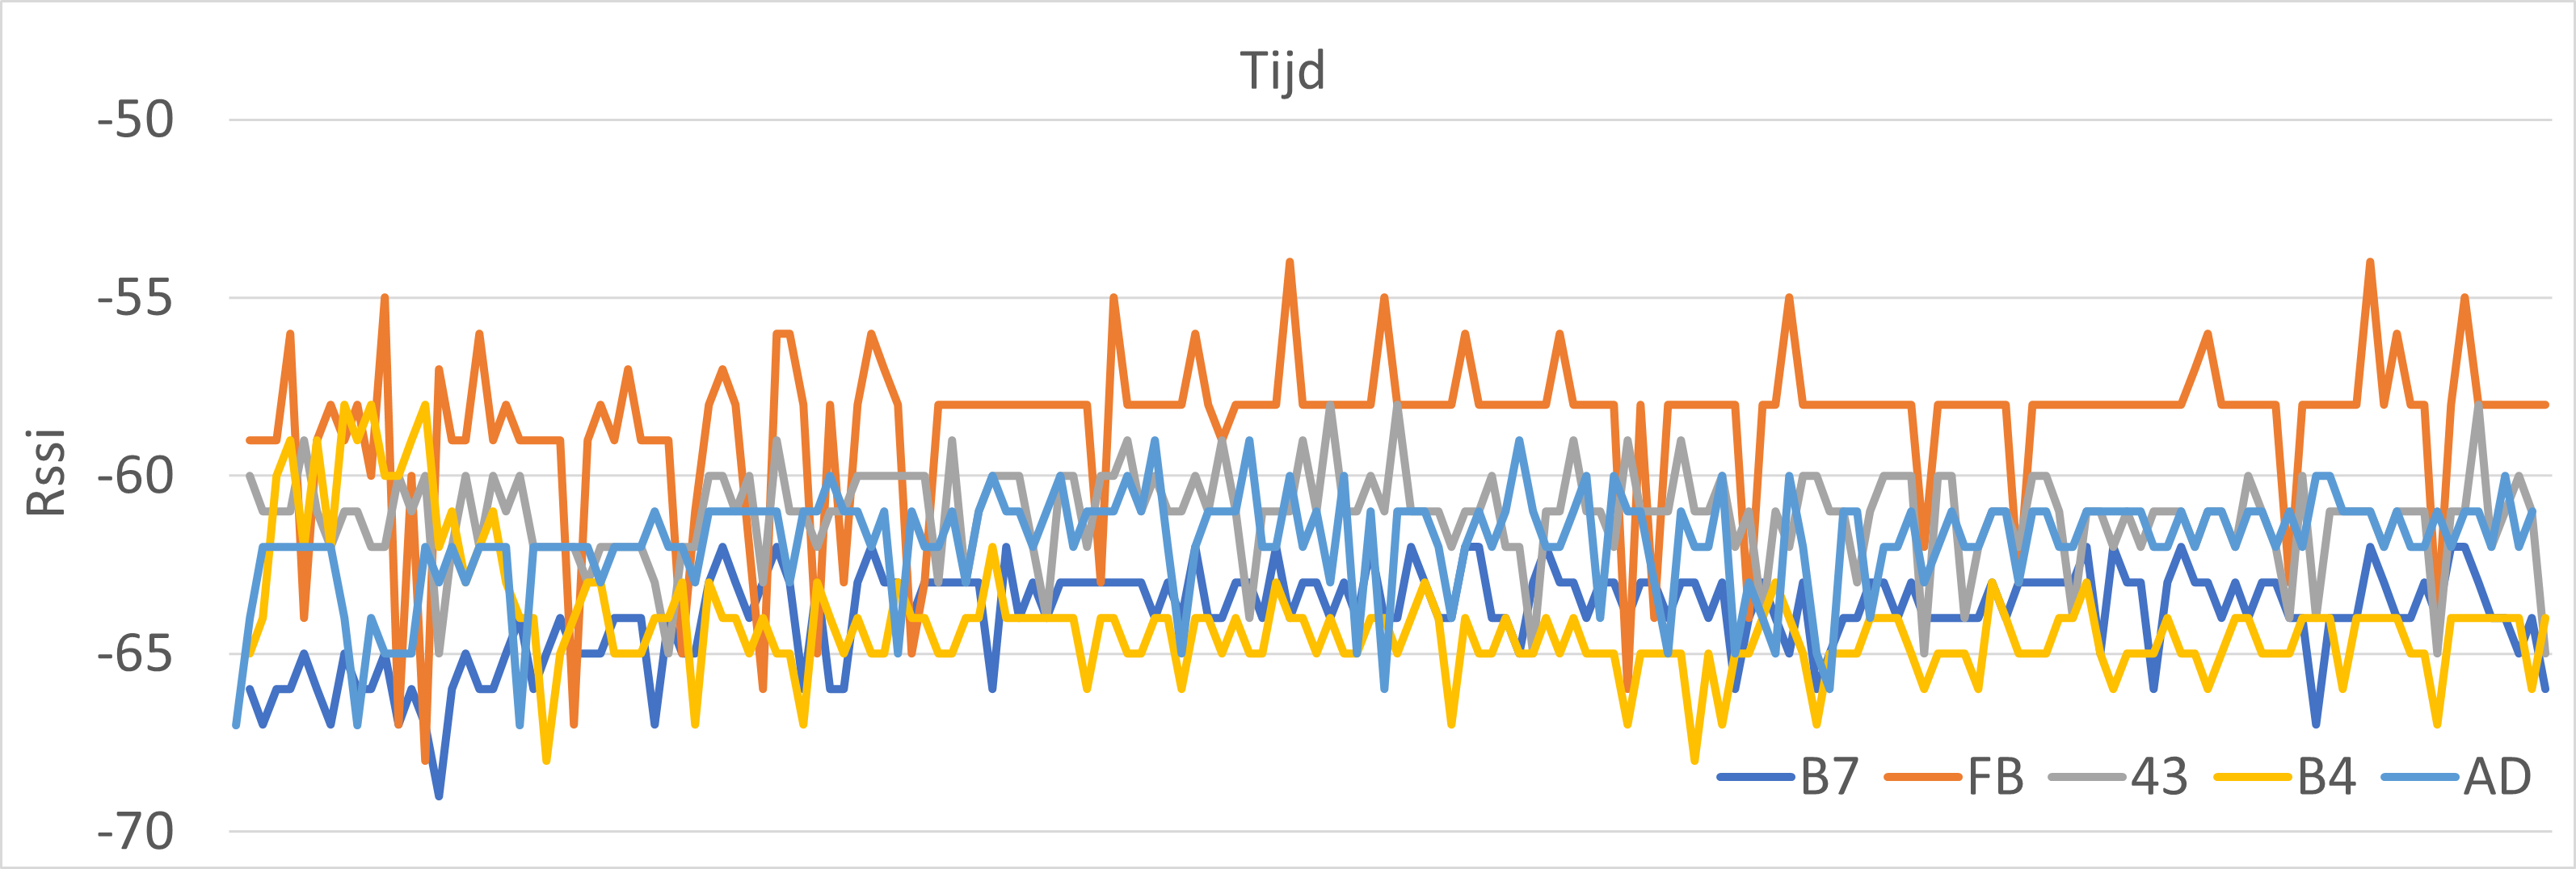
\includegraphics[width=\linewidth]{sble_0_1a}
	\caption{BLE Vooronderzoek - Testresultaat 1a}
	\label{fig:ond-ble-1a-res}
\end{figure}

\paragraph{b) 30 beaconberichten per gatewaybericht}
Uit deze test is zichtbaar dat een uitmiddeling over 30 berichten veel minder variatie geeft, met over het algemeen een variatie van plus en min 1 van de gemiddelde waarde. Dit lijkt meer acceptabel. Ook is er in dit experiment 1 H5 beacon (code AD) vervangen door 2 beacons van het type H2. Dit om een vermoeden te onderzoeken dat, alhoewel alle beacons dezelfde instellingen hebben, hun zendsterkte toch varieert. Dit is hier ook bevestigd, deze 2 (6F en 23) hebben een hogere gemiddelde RSSI waarde dan de 4 overgebleven H5 beacons, welke onderling ook vrij veel van elkaar verschillen.

\begin{figure}[h]
	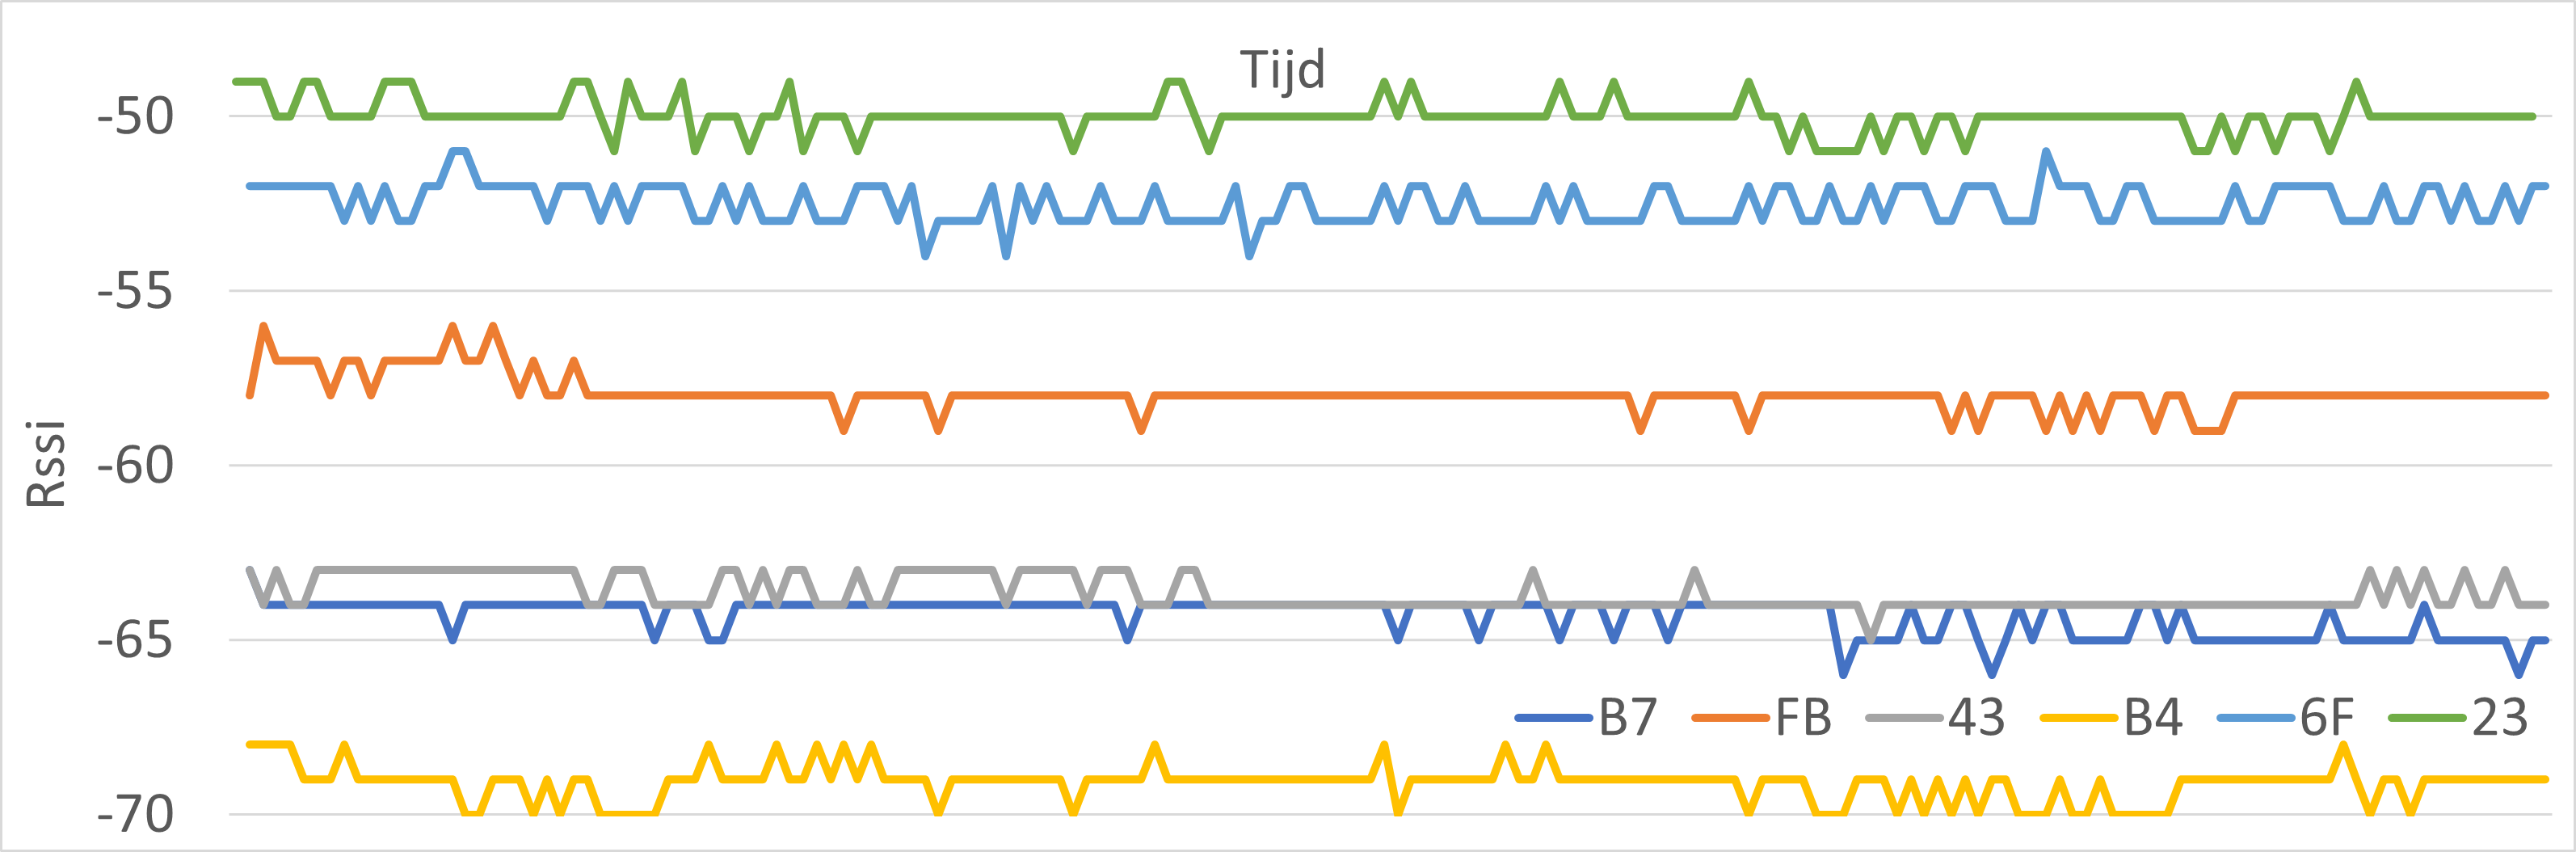
\includegraphics[width=\linewidth]{sble_0_1b}
	\caption{BLE Vooronderzoek - Testresultaat 1b}
	\label{fig:ond-ble-1b-res}
\end{figure}

\paragraph{Testconclusie}
Uit deze eerste test zijn 2 dingen duidelijk geworden, allereerst dat er een goed aantal beaconberichten nodig is voor uitmiddeling per gatewaybericht, anders zijn er grote variaties in de RSSI waarden. Aan het versnellen van de beacons is echter ook een groot nadeel verbonden, namelijk het verminderen van de batterijduur. Deze factor is rechtstreeks verbonden aan kostprijs, voor de nieuwe batterij, en de werkuren om deze te vervangen. Ook zal het afhangen van de use-case hoe belangrijk deze is. Alternatief kan ook de gateway trager uitsturen, wat een negatief effect zal hebben op de lokalisatiesnelheid. Dit zal een afweging zijn gebaseerd op de situatie maar is zeker niet onbelangrijk. Tijdens het verdere verloop van dit onderzoek zal een (arbitraire) waarde van 30 beaconberichten per gatewaybericht worden aangehouden, aangezien dit een mooie middenweg lijkt, maar dit kan duidelijk verhoogd/verlaagd worden met de voor- en nadelen vandien.

Als 2e is er ook duidelijk geworden dat er een verschil zit tussen de zendsterkte van BLE beacons met dezelfde instellingen. Dit zowel voor beacons van hetzelfde type, als van andere types. Hieruit volgt dus dat, als er een omzetting van RSSI waarde naar een afstand moet worden gemaakt, deze waarde op een of andere manier zal moeten worden genormaliseerd. Een mogelijkheid hiervoor is het veld 'RSSI at 0m', aanwezig in een UID bericht. Een andere optie is de beacons kalibreren dat ze even sterk zenden. Ongeacht hoe hier rond wordt gewerkt, blijft het een aandachtspunt.

\subsubsection{Test 2: Afstandstest}
De volgende veronderstelling die zal worden getest, is het verloop van de RSSI waardes, in functie van afstand tussen de beacons en de gateway. In theorie zou deze moeten verlopen volgens de FSPL formule (ongeveer exponentieel, met en neerwaarts traject van ~6dBm per verdubbeling van de afstand). Deze test heeft als doel na te gaan of dit in praktijk ook zo is.
In dit experiment zal een gateway worden opgesteld, met een beacon die steeds verder van deze gateway zal verwijderd worden in intervallen van 50cm. Dit experiment zal 3x worden herhaald, 1x in een ideale omgeving, nl. een anechoïsche kamer\footnote{Een anechoïsche kamer is een kamer waarvan de muren bedekt zijn met speciaal gevormd mousse, meestal puntvormig. Dit is bedoeld om radio- en geluidsgolven zo goed mogelijk te absorberen en zo een kamer te creëren met zo weinig mogelijk reflecties.}, 1x in een open reële omgeving, nl. een bemeubelde huiskamer, en ditzelfde nogmaals, maar met 1 muur tussen, om zo het verwachte negatieve effect van obstakels te controleren. De meting in ideaal geval zal minder meetpunten bevatten dan de reële, omwille van de gelimiteerde grootte van de anechoïsche kamer.

\subsubsection{Resultaat}
Er is duidelijk zichtbaar dat theorie en realiteit veel van elkaar verschillen. De (beperkte) meetpunten van de ideale meting komen zeer goed in de buurt van de theorie, maar vanaf er wordt overgestapt naar een open reële ruimte zijn de resultaten zeer anders. Met als voornaamste bevindingen dat de waarden veel lager liggen dan in theorie, en dat het niet elke waarde dalend is. Wel is aan de bijgetekende logaritmische trendlijn te zijn dat de reële waarden wel een dalend verloop kennen. Verder zien we dat ook de meting met muur een grillig, maar neerwaarts verloop vertoon, op een lager niveau dan zonder muur.

\begin{figure}[h]
	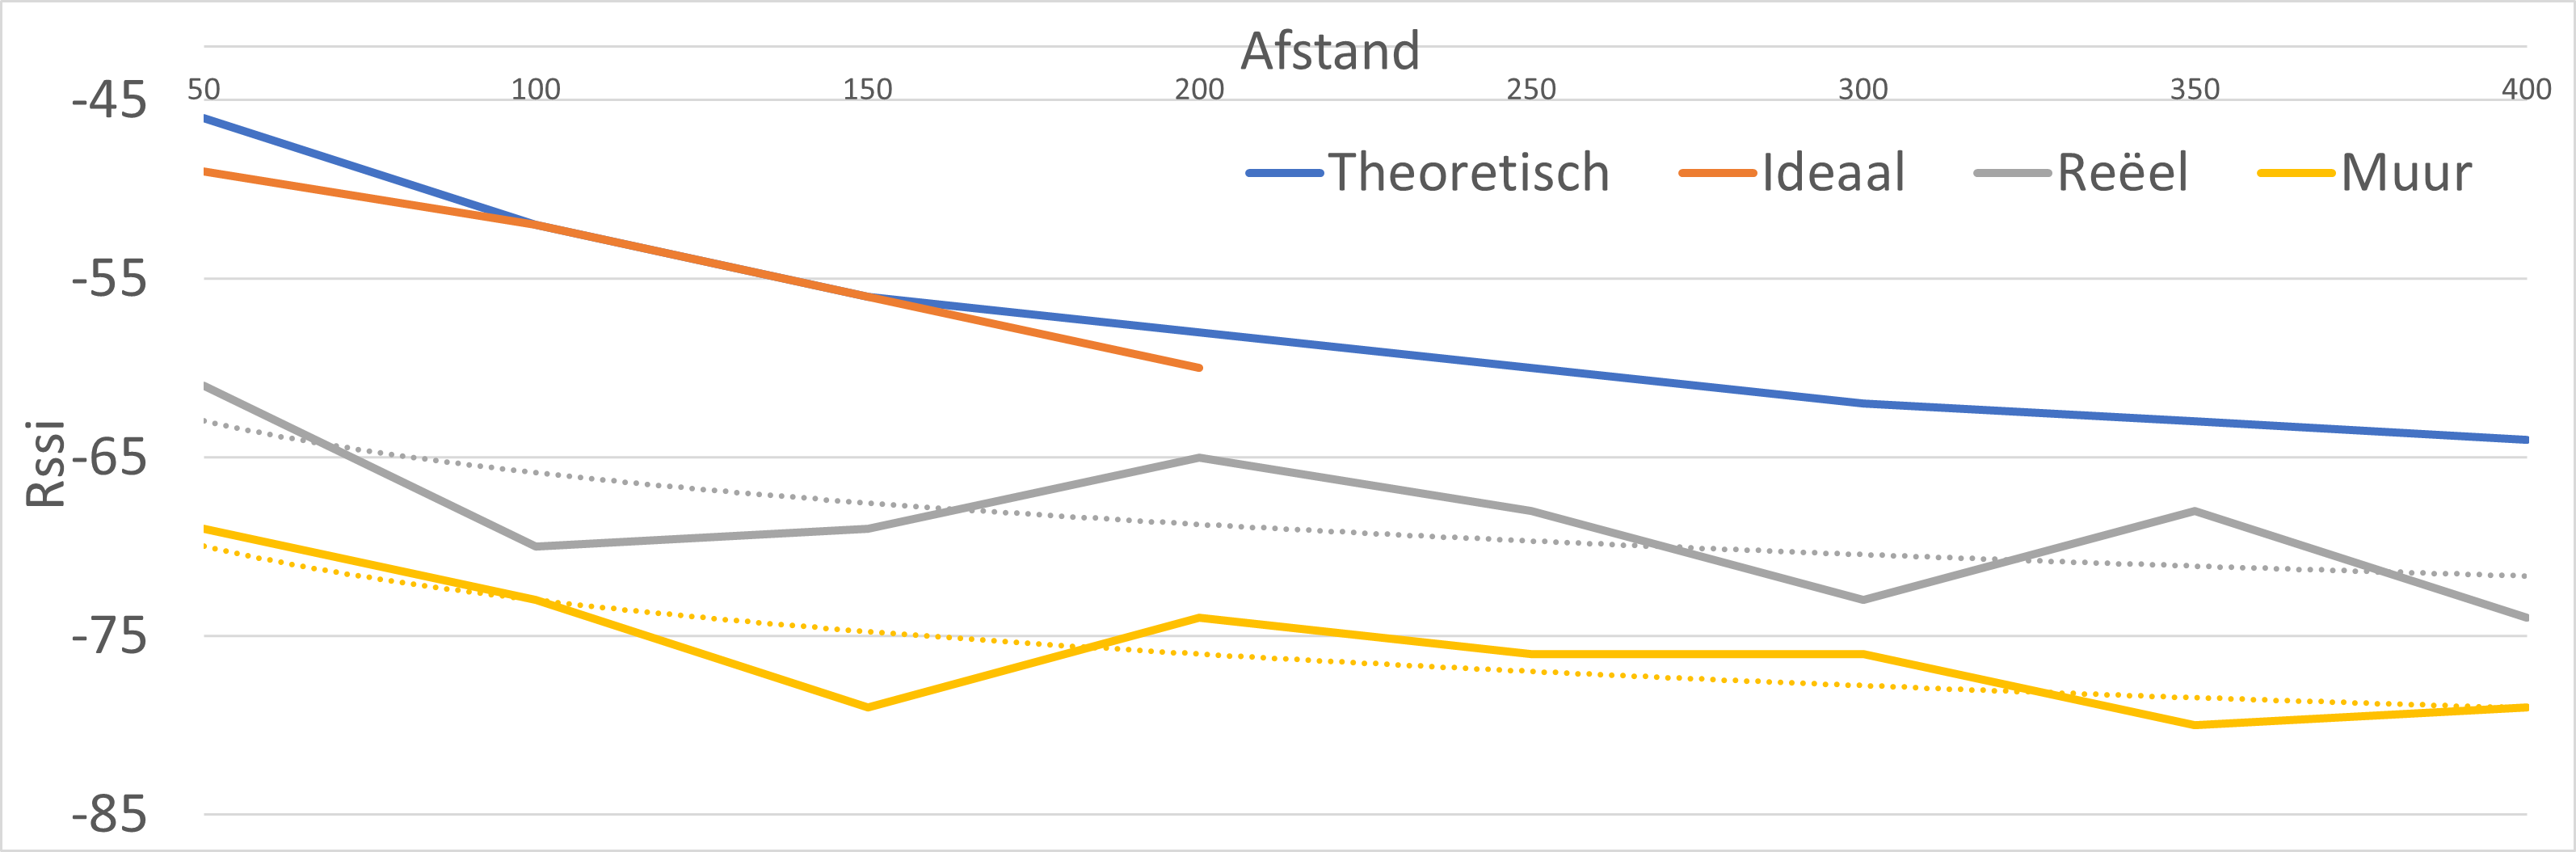
\includegraphics[width=\linewidth]{sble_0_2}
	\caption{BLE Vooronderzoek - Testresultaat 2}
	\label{fig:ond-ble-2-res}
\end{figure}

\emph{De reële testen zijn uitgevoerd met 5 verschillende MokoSmart H5 beacons, echter aangezien allen een gelijkaardig verloop vertoonden, worden de andere 4 niet extra bijgevoegd.}

\paragraph{Testconclusie}
Aangezien het voornaamste verschil tussen de ideale en realistische situatie het bestaan van reflecties is, is met deze test dus duidelijk geworden dat deze een zeer grote impact kunnen hebben op de resultaten en de RSSI waarden. Voornamelijk in de vorm van een schommeling, welke vervelend is als er een conversie moet worden gemaakt tussen RSSI en afstand, en verder ook in een algehele RSSI vermindering tegenover de theorie. 
De testen voor de effectieve scenario's zullen allen plaatsvinden in reële omgevingen, aangezien implementaties van systemen gebaseerd op deze scenario's ook in reële ruimtes zullen werken, en puur theoretische of ideale situaties dus geen nut hebben om te vergelijken.

\subsubsection{Test 3: Rotatietest}
Deze derde en laatste test in dit vooronderzoek zal de veronderstelling testen dat de meting van de gateway richtingsonafhankelijk is, nl. of er een verschil is in RSSI als de enige variabele de locatie van de beacon rond de gateway is.
Voor deze test is een gateway opgesteld op een draaiplatform in een anechoïsche kamer, met een MokoSmart H5 beacon op 150cm afstand. Tijdens te test zal de gateway rond zijn as draaien. Dit gebeurt 2x, eens met de beacon op dezelfde hoogte als de gateway, en eens met de beacon 50cm hoger.

\paragraph{a) Beacon en gateway op zelfde hoogte}

\begin{minipage}{0.55\textwidth}
Uit dit resultaat is zeker duidelijk dat er een zekere richtingsafhankelijk is, met een grote blindspot rond 260° van -68 dBm, een verschil met het gemiddelde van 10dBm, met 2 kleinere op 80° en 180° met een verschil van 5 dBm. Alhoewel niet drastisch, het overgrote deel van is vrij constant, is dit toch noemenswaardig. De meest voor de hand liggende verklaring hiervoor is het feit dat de ingebouwde (staaf) antenne loopt op de lijn van 90° en 270°, dus de 2 voornaamste dippen wijzen ongeveer naar de uiteinden van deze antenne, en een blindspot hier is karakteristiek voor een staafantenne.
\end{minipage}
\hfill
\begin{minipage}{0.42\textwidth}
	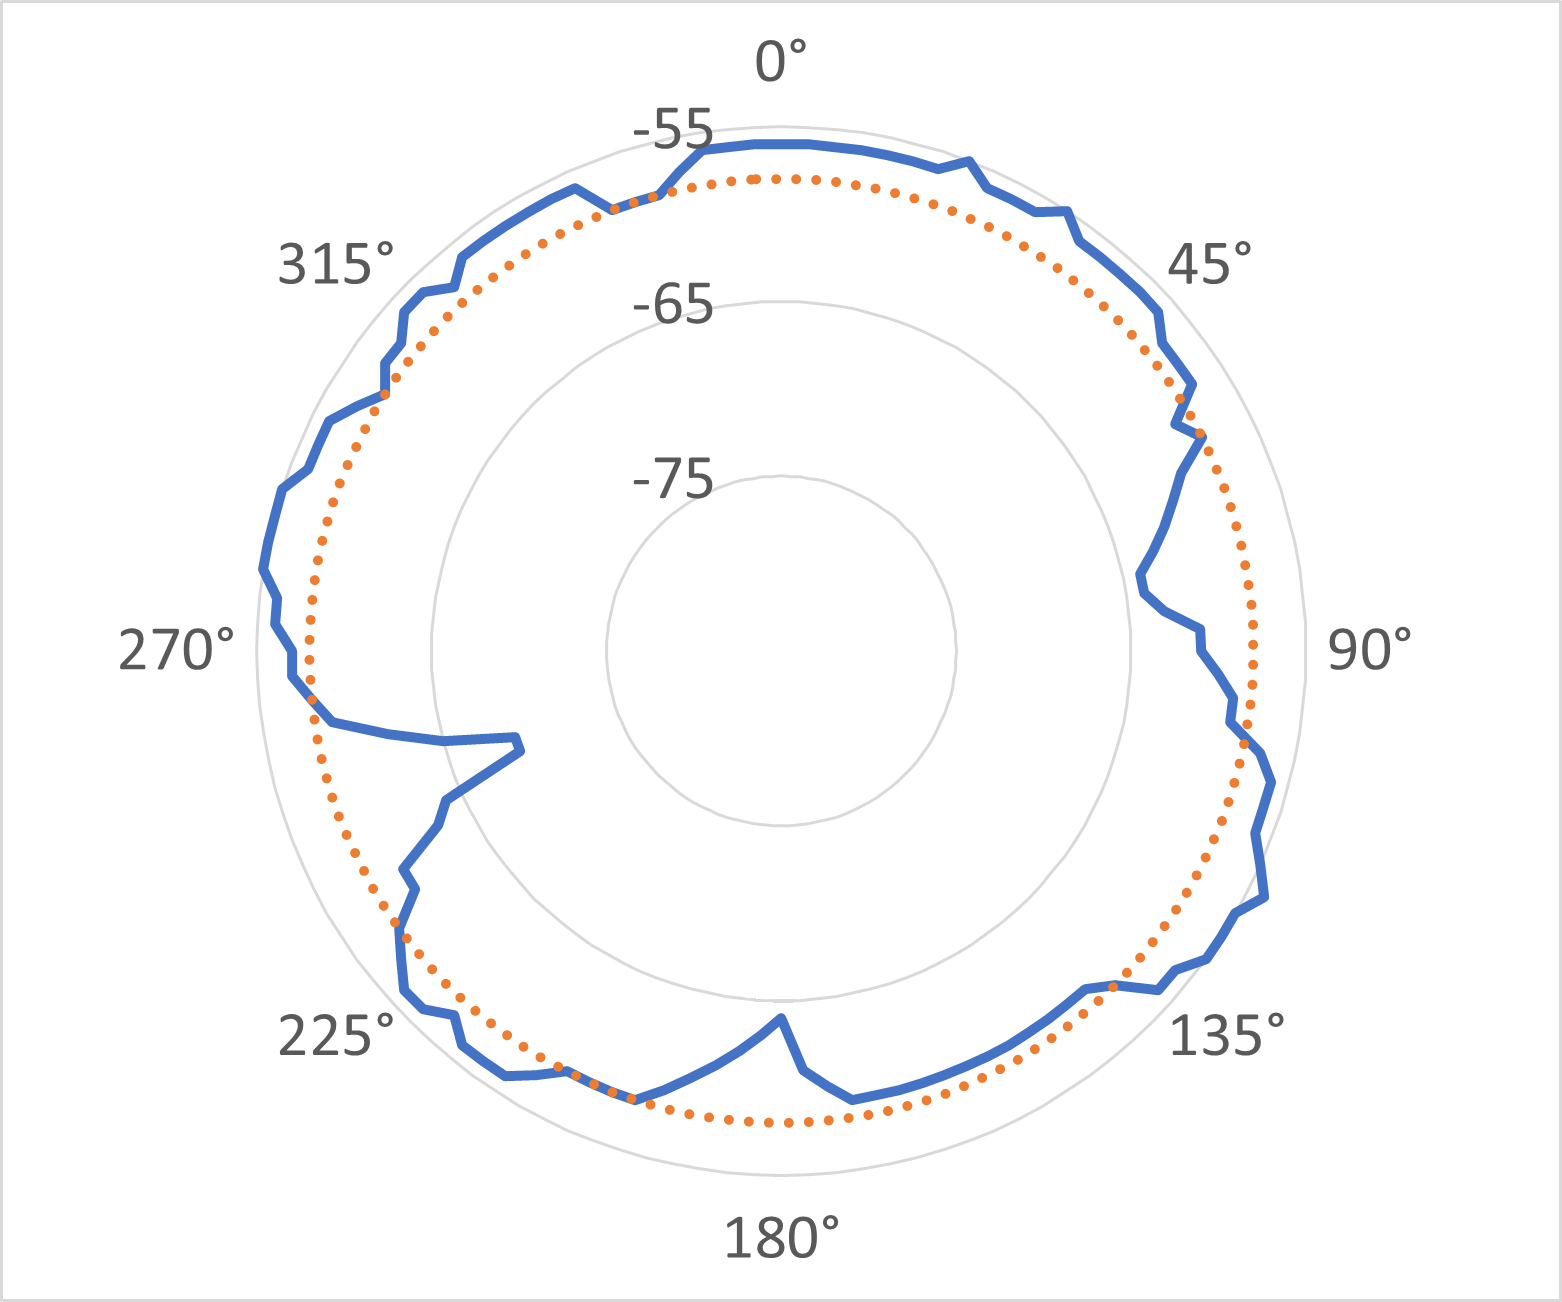
\includegraphics[width=\linewidth]{sble_0_3a}
	\captionof{figure}{BLE Vooronderzoek - Testresultaat 3a}
	\label{fig:ond-ble-3a-res}
\end{minipage}


\paragraph{b) Beacon 50cm boven gateway}

\begin{minipage}{0.55\textwidth}
Hier is zichtbaar dat de harde blindspots uit de vorige test verdwenen zijn, wat het vermoeden dat dit met de antennerichting te maken heeft lijkt te bevestigen. Wel is er nog een duidelijk dal in het kwartaal tussen 225° en 315°.
\end{minipage}
\hfill
\begin{minipage}{0.42\textwidth}
	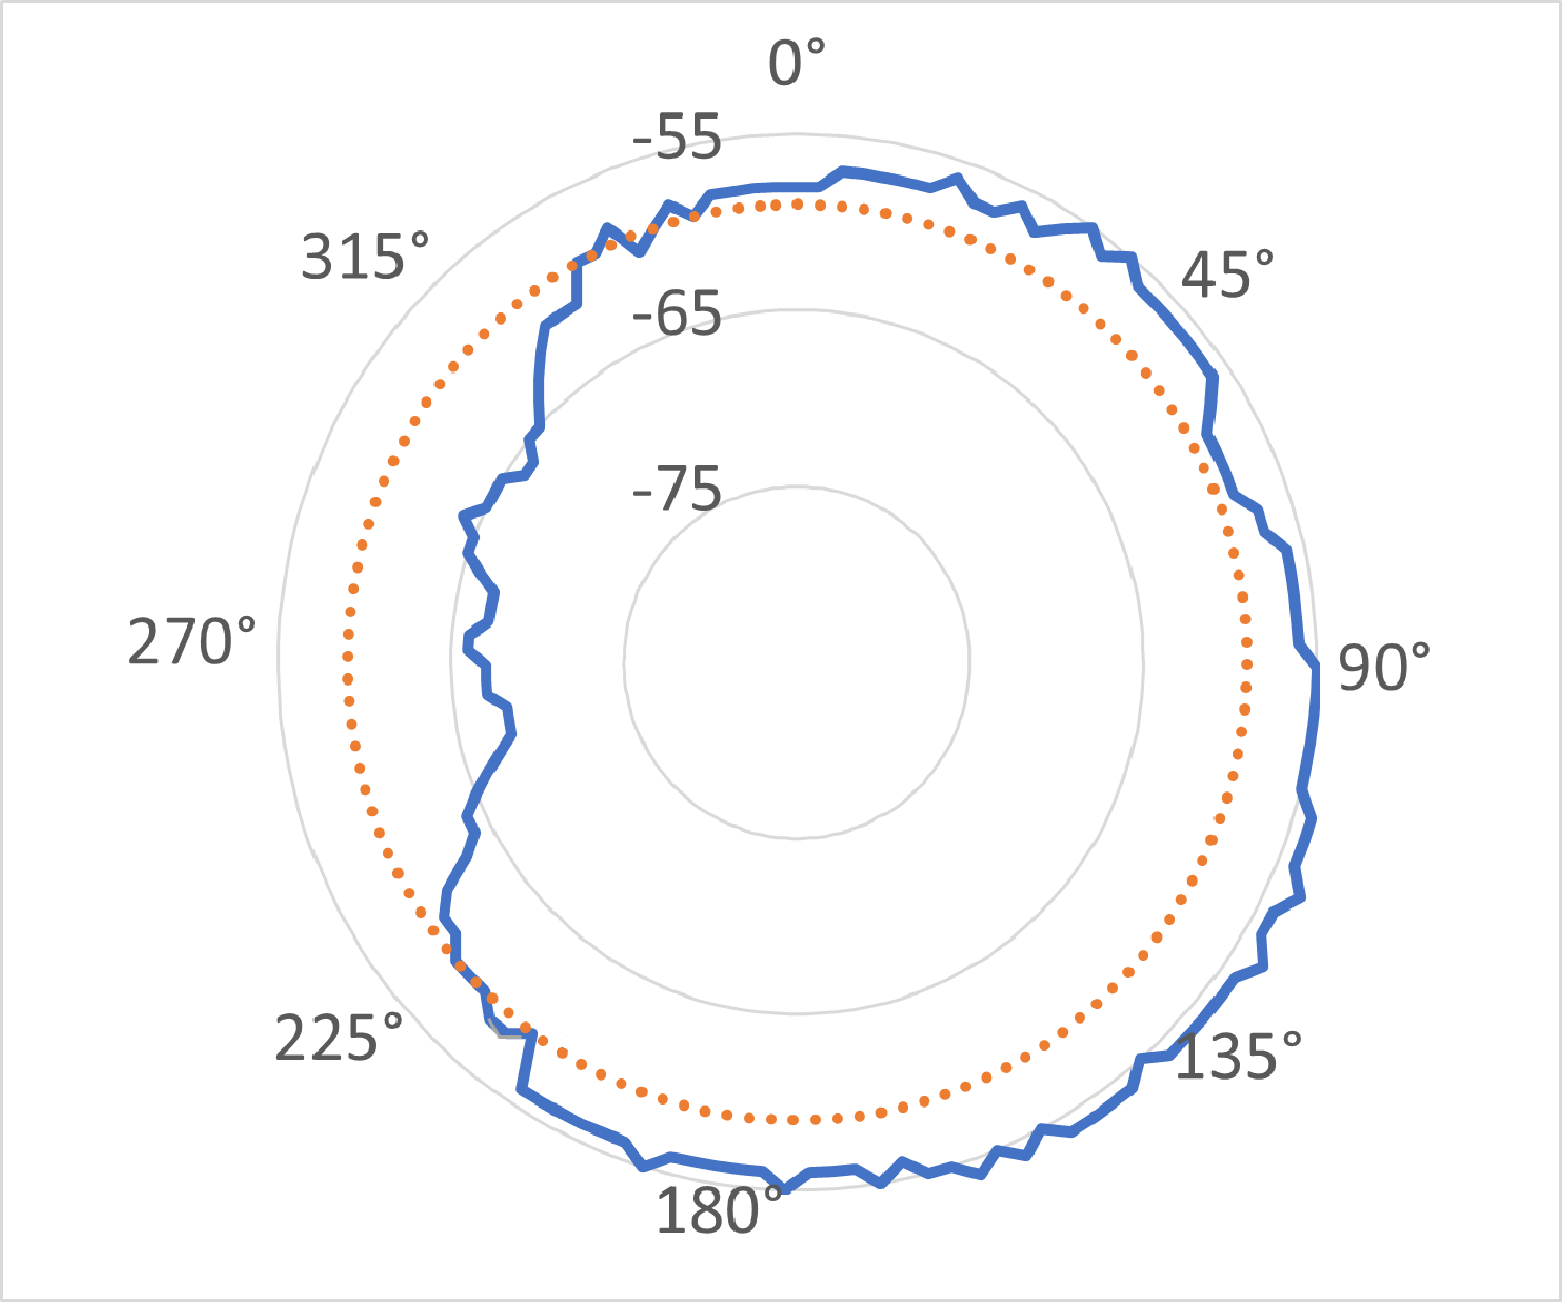
\includegraphics[width=\linewidth]{sble_0_3b}
	\captionof{figure}{BLE Vooronderzoek - Testresultaat 3b}
	\label{fig:ond-ble-3b-res}
\end{minipage}

\paragraph{Testconclusie}
Uit deze test is duidelijk geworden dat een gateway niet 100\% richtingsonafhankelijk is. Over de grote lijn zal dit vermoedelijk geen problemen geven, echter kunnen de plotse daten in meetgevoeligheid onverwachte waarden opleveren als een beacon toevallig net in die richting ligt.
Tijdens de volgende testen zullen alle gateways in dezelfde richting worden geplaatst om het effect van deze verlopen te standaardiseren. 

\subsubsection{Deelconclusie}
Uit dit vooronderzoek is duidelijk geworden dat niet elke theoretische veronderstelling ook geldig is in een reële praktijk. Het is belangrijk dit eerst vastgesteld te hebben, aangezien het waarschijnlijk mogelijk zal zijn om sommige anders onverklaarbare fenomenen in komende scenariotests te verklaren. Ook zijn er in de testconclusies maatregelen/standaarden vastgelegd om deze effecten zo veel mogelijk te standaardiseren.

\section{Statische BLE}
\subsection{1 gateway per locatie}
\subsubsection{Deelhypothese}
Deze opstelling zal een asset kunnen lokaliseren, genomen dat de gekozen locaties een gelijkaardige grootte hebben.

\subsubsection{Test 1: 6 locaties in reële, open ruimte, gelijk verdeeld}
\begin{minipage}{0.55\textwidth}
De eerste test voor deze opstelling bestaat uit de eenvoudigste en best case opstelling. In een open ruimte zijn, in een raster, 6 gateways\footnotemark geplaatst, op een afstand van 2m uit elkaar. Dan is de ruimte in 6 locaties verdeeld, volgens de afstand van de beacons. Een punt behoort dus tot de locatie van de dichtstbijliggende gateway. In praktijk komt deze locatieafscheiding\footnotemark neer op een raster middendoor de gateways. Verder worden er verschillende MokoSmart H5 en M2 beacons verdeeld over de ruimte, en zal worden bekeken waar zij volgens de gemeten waarden zich bevinden, en zal dit worden vergeleken met hun echte positie.
\end{minipage}
\footnotetext{Gateways worden aangeduid door een grijs blokje met een bijhorende letter. De illustratie is ook voorzien van 2 rode stippen op de gateway, deze illustreren de voorkant (0°) van de gateway.}
\footnotetext{De grenzen van locaties worden in de illustraties aangegeven door een stippellijn.}
\hfill
\begin{minipage}{0.42\textwidth}
	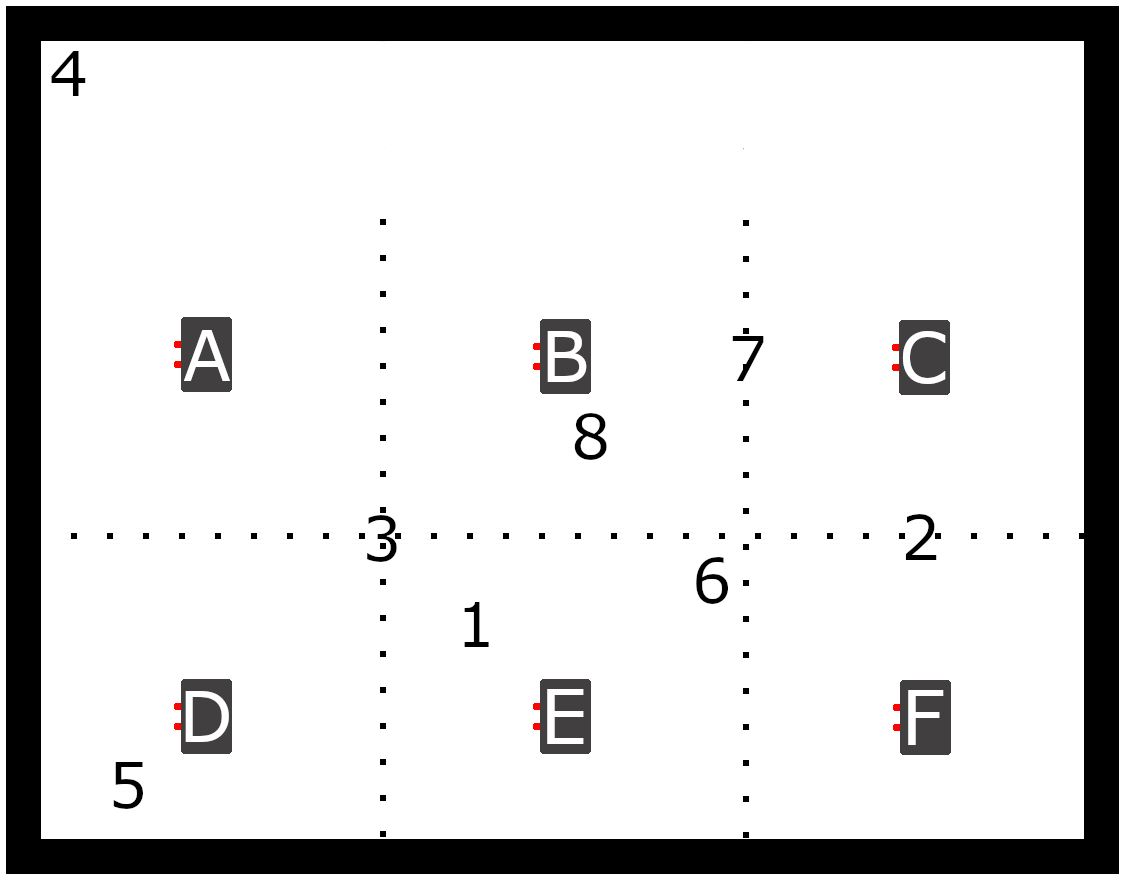
\includegraphics[width=\linewidth]{sble_1_1_floor}
	\captionof{figure}{1 gateway per locatie - Opstelling 1}
	\label{fig:ond-ble-static-1-1-ops}
\end{minipage}

\paragraph{Resultaat}
\begin{minipage}{0.55\textwidth}
De resultaten van deze test zijn zichtbaar in bijhorende tabel. De laagste waarden per beacon staan aangeduid in het groen, en het is meteen duidelijk dat deze toewijzing over het algemeen goed is verlopen. Ook grensgeval beacons zijn toegewezen aan 1 van hun aangrenzende locaties. Enkel bij beacon 6 en 8 is een verschil te vinden.
\end{minipage}
\hfill
\begin{minipage}{0.42\textwidth}
	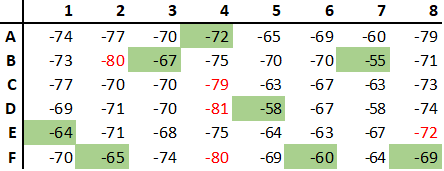
\includegraphics[width=\linewidth]{sble_1_1_results}
	\captionof{figure}{1 gateway per locatie - Testresultaat 1}
	\label{fig:ond-ble-static-1-1-res}
\end{minipage}

We hebben een onderscheid in soorten beacons die even apart horen besproken te worden, in volgorde van moeilijkheid. Allereerst hebben we beacons die duidelijk in een locatie liggen, niet tussen 2 beacons. Tijdens deze test zijn dit beacon 4 en 5. Deze zijn beiden met een comfortabel RSSI verschil gecategoriseerd in de juiste locatie. Verder hebben we de beacons duidelijk in een locatie, maar tussen verschillende gateways. Dit zijn beacons 1 en 8. Hoewel beacon 1 met voorsprong correct is, is er iets vreemd gebeurd bij beacon 8, welke gecategoriseerd wordt bij gateway F, van een zelfs niet aangrenzende locatie.  Dit is zeer vreemd aangezien deze zeer dicht bij gateway B lag, maar als we dit vergelijken met het meetpatroon van de gateway zien we dat deze toevallig net in een blindspot lijkt te liggen, wat een mogelijke verklaring zou kunnen zijn. Verder zijn er de grensgeval beacons, waaronder beacon 2 en 7, welke op de grens tussen 2 locaties liggen. Zij zijn echter toegewezen aan 1 van deze 2, welke in orde is, aangezien het in dit scenario niet de bedoeling is om een exacte positie te bepalen, maar toewijzing aan een locatie te doen. En als laatste beacon 3 en 6 op een 4-punt. Beacon 3 is ook aangrenzend toegewezen dus ook in orde. Beacon 6, alhoewel fysiek net over de grens van locatie E liggend, is toegewezen aan aangrenzende locatie F. In theorie is dit dus een fout, maar geen grote. Ook is een zekere foutmarge bij de locatiegrenzen geen verassing, gezien de onzekerheden in de RSSI waarden vastgesteld in het vooronderzoek.

\paragraph{Testconclusie}
De eerste test heeft bewezen dat dit lokalisatiescenario mogelijkheden heeft, op zijn minst in een eenvoudige egale opstelling. Een toewijzingsscore van 6.5/8 is ook zeker acceptabel.

\subsubsection{Test 2: 6 even grootte in reële, open ruimte, ongelijk verdeeld}
\begin{minipage}{0.55\textwidth}
Deze test verandert de locaties van gelijke grootte uit vorige test in locaties van variabele grootte en vorm. Verder is de ruimte, hoewel nog steeds open, niet meet convex. De locaties blijven dit wel. Hier is het dus niet zo dat elk punt zich ook bij zijn dichtstbijzijnde gateway bevind qua locatie.
\end{minipage}
\hfill
\begin{minipage}{0.42\textwidth}
	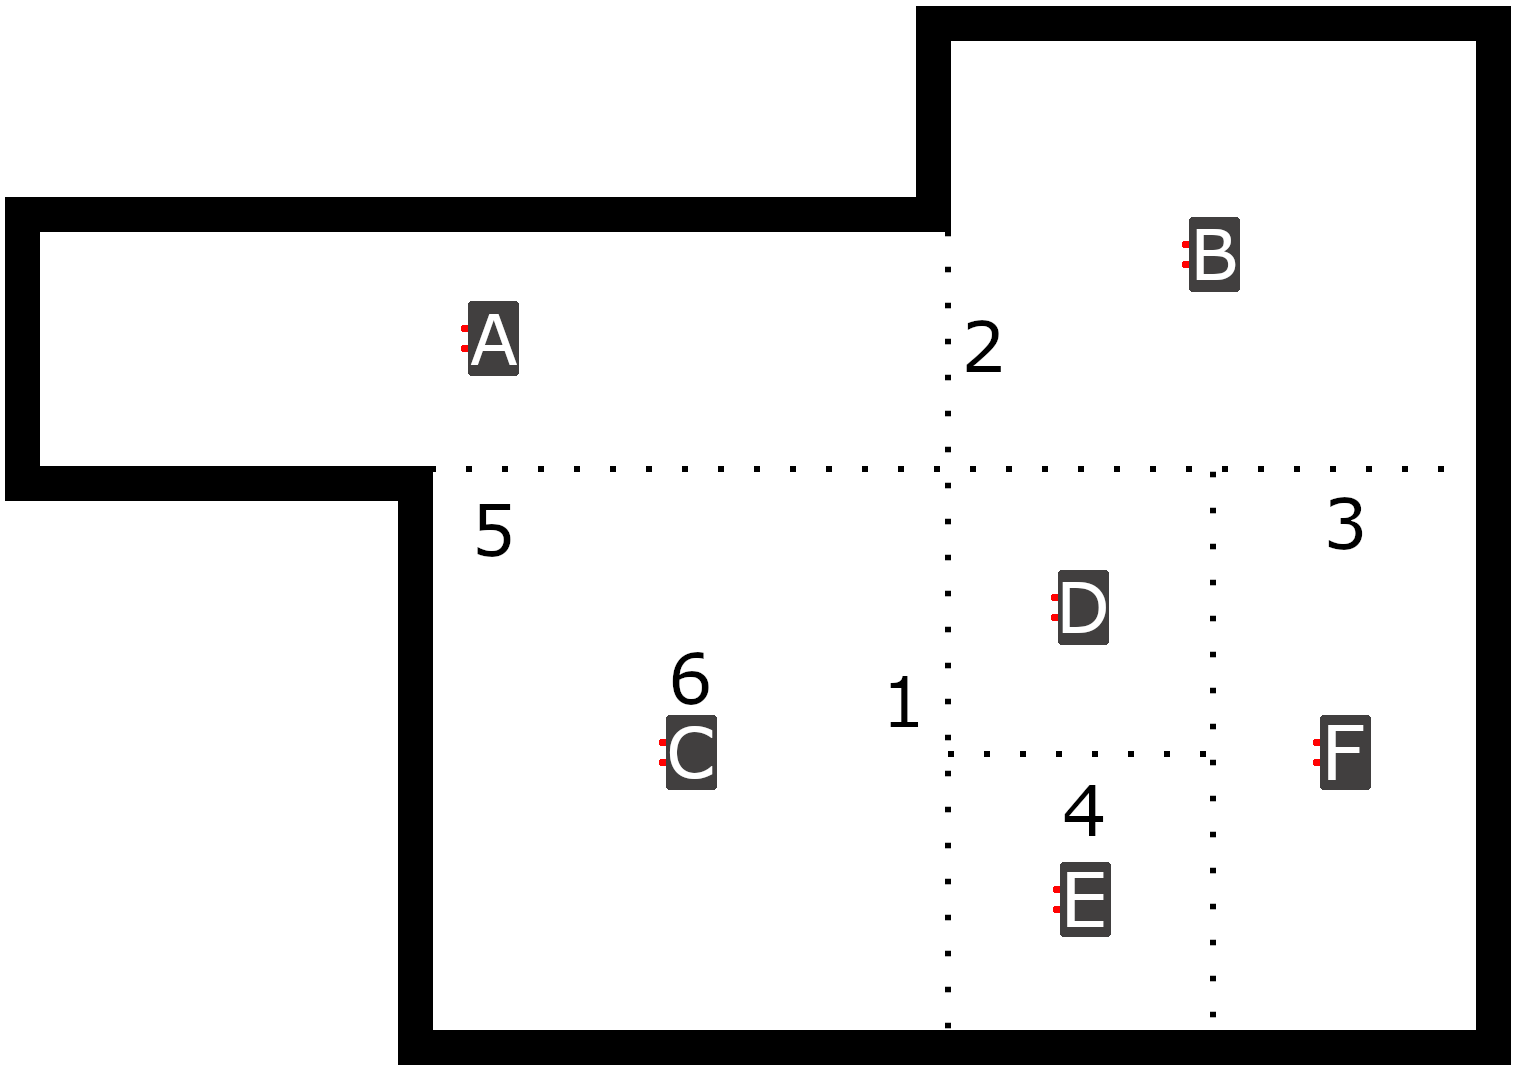
\includegraphics[width=\linewidth]{sble_1_3_floor}
	\captionof{figure}{1 gateway per locatie - Opstelling 2}
	\label{fig:ond-ble-static-1-3-ops}
\end{minipage}

\paragraph{Resultaat}
\begin{minipage}{0.55\textwidth}
De resultaten van deze test zijn zichtbaar in bijgevoegde tabel. We zien dat van de 6 beacons er 3 goed en 3 slecht zijn toegewezen. Echter zijn de 3 slecht toegewezen beacons (1, 3 en 5) de beacons die dichter lagen bij de toegewezen locatie gateway dan bij de theoretisch correcte locatie gateway. De andere 3 beacons (2, 4 en 6) zijn wel correct toegewezen. 
\end{minipage}
\hfill
\begin{minipage}{0.42\textwidth}
	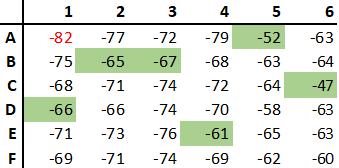
\includegraphics[width=\linewidth]{sble_1_3_results}
		\captionof{figure}{1 gateway per locatie - Testresultaat 2}
	\label{fig:ond-ble-static-1-3-res}
\end{minipage}

\paragraph{Testconclusie}
Deze test bevestigd het vermoeden dat deze lokalisatie strategie het slechter zal doen bij locaties van verschillende groottes, door de basering op RSSI en afstand, en dit zeker in een open ruimte waar deze afstand de enige bepalende factor voor de RSSI is (uiteraard buiten de onzekerheden vastgesteld tijdens het BLE vooronderzoek). Een mogelijke remedie hiervoor is ee RSSI filter te plaatsen op gateways voor kleinere locaties, zodat het gebied dat ze (stelen) van aanpalende grotere ruimtes verminderd. Echter omdat het bereik nog steeds (theoretisch) een cirkel blijft zullen vreemde verschijnsels bij locatieovergangen onvermijdelijk blijven.

\subsubsection{Test 3: 5 realistische locaties}
\begin{minipage}{0.55\textwidth}
Deze derde een laatste test vergroot het concept vn vorige test en voegt muren toe zodat de opstelling realistischer wordt. Deze opstelling bestaat uit 5 locaties, ondergebracht in 5 ruimtes van verschillende groottes, gescheiden door muren. Hier is dus afstand niet meer de enige bepalende factor voor de RSSI, maar ook tussenliggende muren. Wat in theorie een groter verschil zou moeten geven, en het grootteverschil tussen locaties wat zou kunnen compenseren. Dit experiment zal ook 2x worden uitgevoerd, 1x met tussenliggende deuren gesloten, en 1x open, om ook het mogelijke effect van deuren vast te stellen.
\end{minipage}
\hfill
\begin{minipage}{0.42\textwidth}
	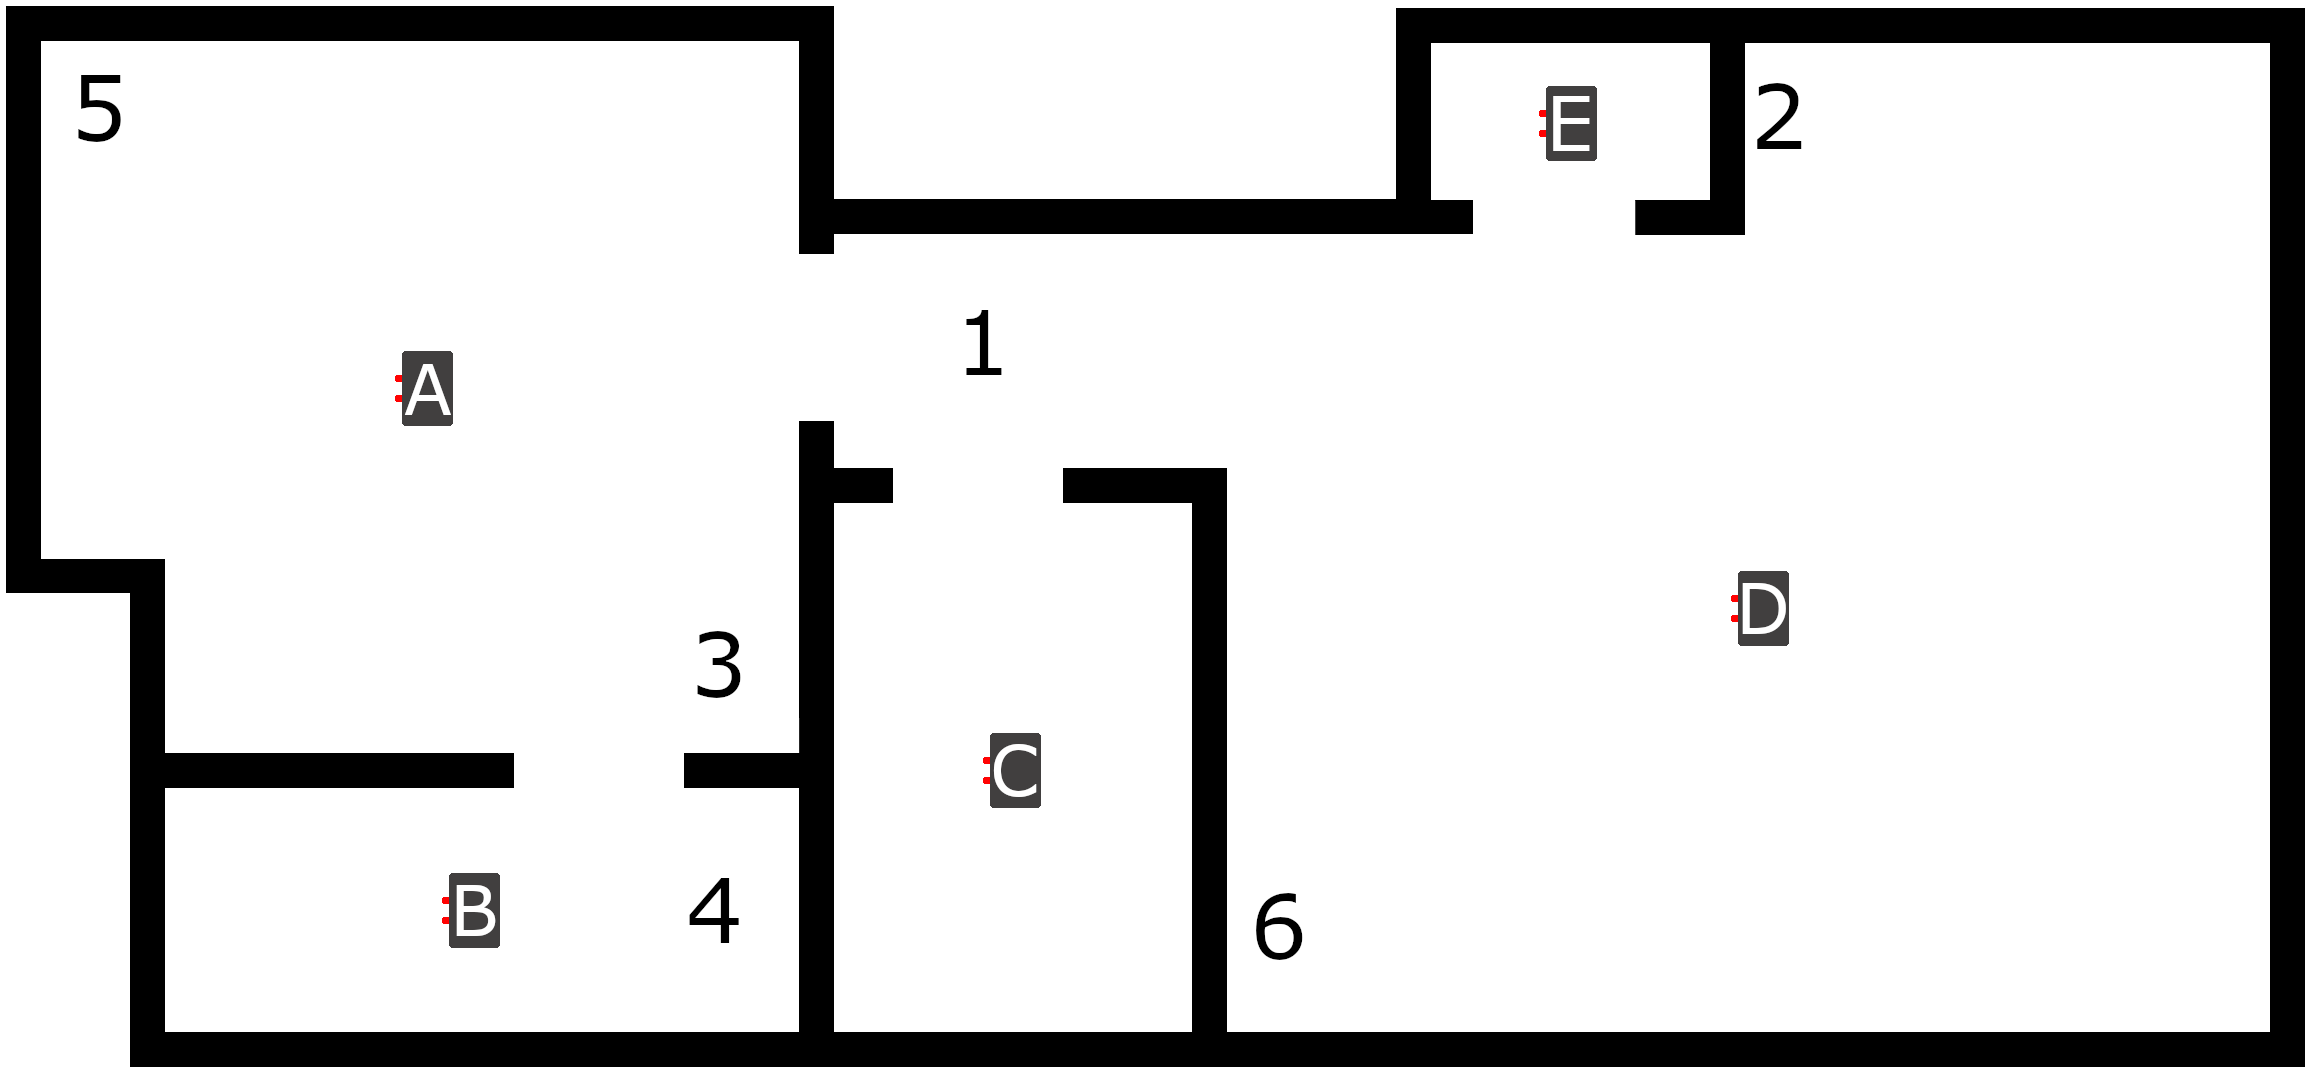
\includegraphics[width=\linewidth]{sble_1_4_floor}
	\captionof{figure}{1 gateway per locatie - Opstelling 3}
	\label{fig:ond-ble-static-1-4-ops}
\end{minipage}

\paragraph{a) Deuren gesloten}
\begin{minipage}{0.55\textwidth}
Uit de resultaten is af te leiden dat dit principe zeer goed werkt, met een perfecte lokalisatie. Dit is geen verassing voor da duidelijke, safe beacons (4 en 5). Maar de andere 4 beacons liggen stuk voor stuk in een locatie maar dichter bij een andere gateway (weliswaar met een muur tussen). Met in het bijzonder beacon 2, welke op ong 50cm (+muur) ligt van gateway E, en op 250cm van gateway D, maar nog steeds correct bij locatie D wordt gecategoriseerd.
\end{minipage}
\hfill
\begin{minipage}{0.42\textwidth}
	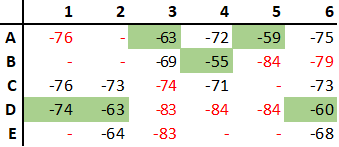
\includegraphics[width=\linewidth]{sble_1_4a_results}
	\captionof{figure}{1 gateway per locatie - Testresultaat 3a}
	\label{fig:ond-ble-static-1-4a-res}
\end{minipage}

\paragraph{b) Deuren open}
\begin{minipage}{0.55\textwidth}
Deze resultaten tonen geen noemenswaardig verschil met de test met gesloten deuren. Alles blijft correct gecategoriseerd, maar ook de waardes verschillen niet veel. Dit is vooral verrassend bij beacon 1, welke met open deur rechtstreeks zichtbaar is voor gateway A, maar toch correct bij gateway D blijft ingedeeld.
\end{minipage}
\hfill
\begin{minipage}{0.42\textwidth}
	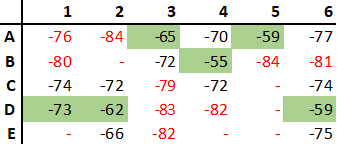
\includegraphics[width=\linewidth]{sble_1_4b_results}
	\captionof{figure}{1 gateway per locatie - Testresultaat 4b}
	\label{fig:ond-ble-static-1-4b-res}
\end{minipage}

\paragraph{Testconclusie}
Deze test toont mooi aan dat de extra isolatie van een muur een positieve invloed heeft op lokalisatie volgens dit principe, en dat een verschil in grote tussen aanpalende ruimtes niet noodzakelijk een groot probleem hoeft te zijn. Uiteraard zal ook het soort muur een invloed hebben op deze resultaten. In de testopstelling worden muren uit cellenbeton gebruikt, maar een dunnere muur uit bv. kalkplaat zal mogelijk een minder isolerend effect hebben. Ook is duidelijk dat een deur weinig impact heeft op de resultaten. Ook dit kan natuurlijk aan het materiaal liggen. Een houten deur zoals in de testopstelling is klaarblijkelijk verwaarloosbaar, maar bv. een nooddeur, speciaal als er metaal in zit, zal een grotere impact hebben.

\subsubsection{Deelconclusie}
Al bij al is dit een zeer acceptabel scenario, het merendeel van de lokalisaties was geslaagd, met uitzondering van fouten aan de locatieovergang in een open ruimte, maar dat is geen verassing na de vaststellingen in het vooronderzoek. Ook bestaat er de mogelijkheid tot toevallige mislokalisaties door hardware effecten, maar dit ligt niet zozeer aan het scenario zelf. De hypothese is bevestigd.

\subsection{Meerdere gateways per locatie}
\subsubsection{Deelhypothese}
Deze opstelling slaagt er in om met een BLE beacon getagde assets correct te lokaliseren.

\subsubsection{Test 1: 2 rechthoekige locaties in reële, open ruimte}
\begin{minipage}{0.55\textwidth}
De testopstelling voor deze eerste test bestaat uit een raster van 6 gateways (analoog aan de opstelling bij het vorige scenario, test 1). De locatiedefinitie is in dit geval in de vakken tussen de gateways, om 2 even grote locaties te creëren. Het idee is dat zichtbaar is aan de meetwaarden in welk vak een beacon ligt, en dus zo een locatie toegewezen krijgt. Meer specifiek aan de laagste som van RSSI's van de gateways in de hoekpunten. 
\end{minipage}
\hfill
\begin{minipage}{0.42\textwidth}
	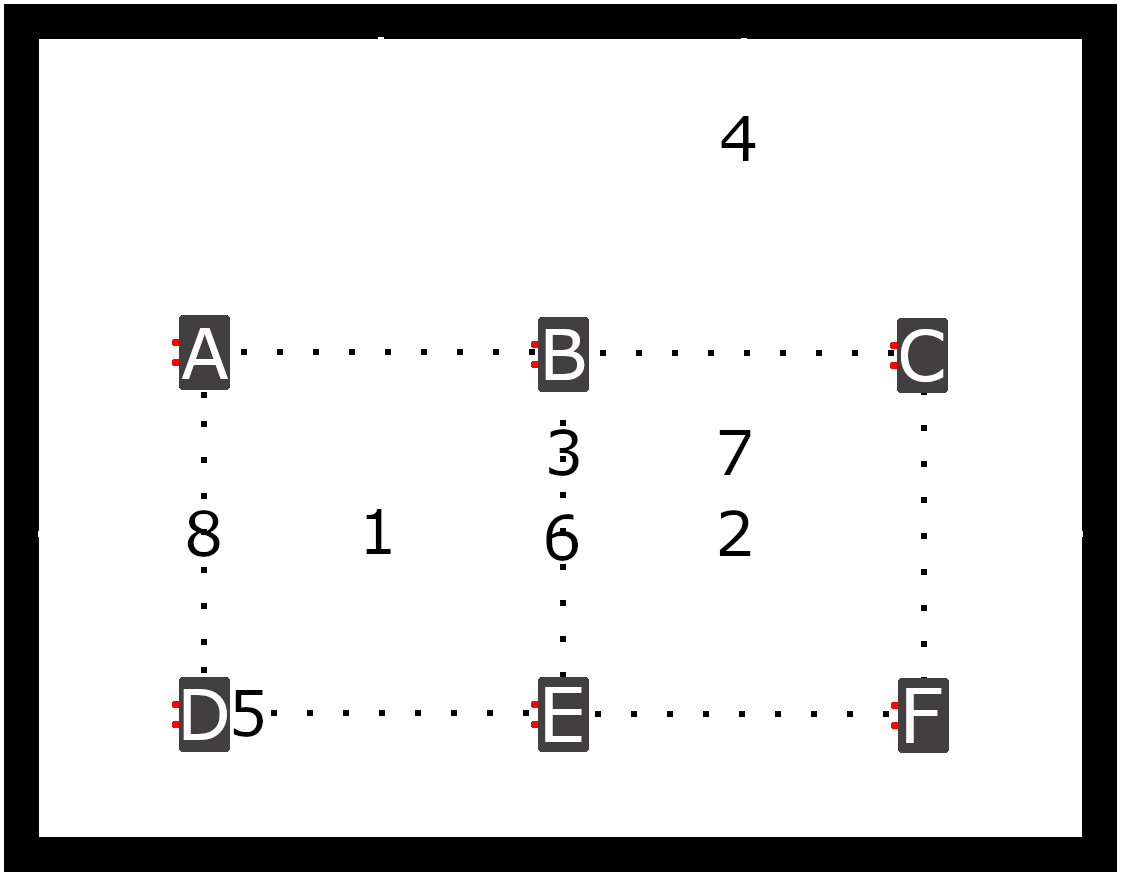
\includegraphics[width=\linewidth]{sble_2_1_floor}
	\captionof{figure}{Meerdere gateways per locatie - Opstelling 1}
	\label{fig:ond-ble-static-2-1-ops}
\end{minipage}

\paragraph{Resultaat}
Bijhorende resultaten zijn verrassend goed, met voor elke van de 8 beacons een correcte lokalisatie. Enkele interessante randgevallen zijn beacon 3 en 6, welke op de grens tussen de 2 locaties liggen. Bij beide zijn de cijfers duidelijk voor de rechtse locatie, nochtans zou men verwachten dat deze cijfers dichter bijeen zouden liggen. Verder is er ook beacon 4, welke op geen enkele locatie ligt en is ingedeeld bij de rechtse locatie. Deze indeling is uiteindelijk de correcte, aangezien dit de dichtstbijzijnde locatie betreft en er geen 'geen locatie' mogelijk is in dit experiment. 

\begin{figure}[h]
	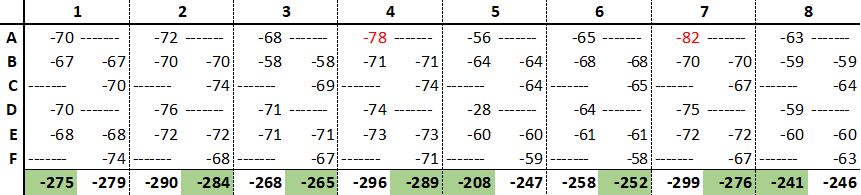
\includegraphics[width=\linewidth]{sble_2_1_results}
	\caption{Meerdere gateways per locatie - Testresultaat 1}
	\label{fig:ond-ble-static-2-1-res}
\end{figure}

\paragraph{Testconclusie}
Deze opstelling heeft in deze eerste test een perfecte lokalisatie gedaan, en is daarmee voorlopig zeer goed. Echter is er het detail van de 'geen locatie' beacons, maar dit is in elk scenario een ding. Hier is dit in theorie oplosbaar aangezien er een bepaalbare bovengrens in som van RSSI's wil de beacon nog tussen de gateways liggen. Deze is ook theoretisch berekenbaar gegeven de afstand tussen de gateways, de FSPL formule en enige meetkundige kennis, maar gezien het vastgestelde verschil tussen theorie en praktijk tijdens het vooronderzoek lijkt dit eerder een maximum dat moet worden gemeten/bepaald.

\subsubsection{Test 2: 2 rechthoekige locaties gescheiden door muur}
\begin{minipage}{0.55\textwidth}
De opstelling voor deze test is analoog an de vorige, het enige verschil is dat er een muur is verschenen tussen de 2 locaties. Dit zal in praktijk ook meer het geval zijn, nl. 2 aanpalende lokalen. Het doel van deze test is om het effect van deze muur op de cijfers te bekijken.
\end{minipage}
\hfill
\begin{minipage}{0.42\textwidth}
	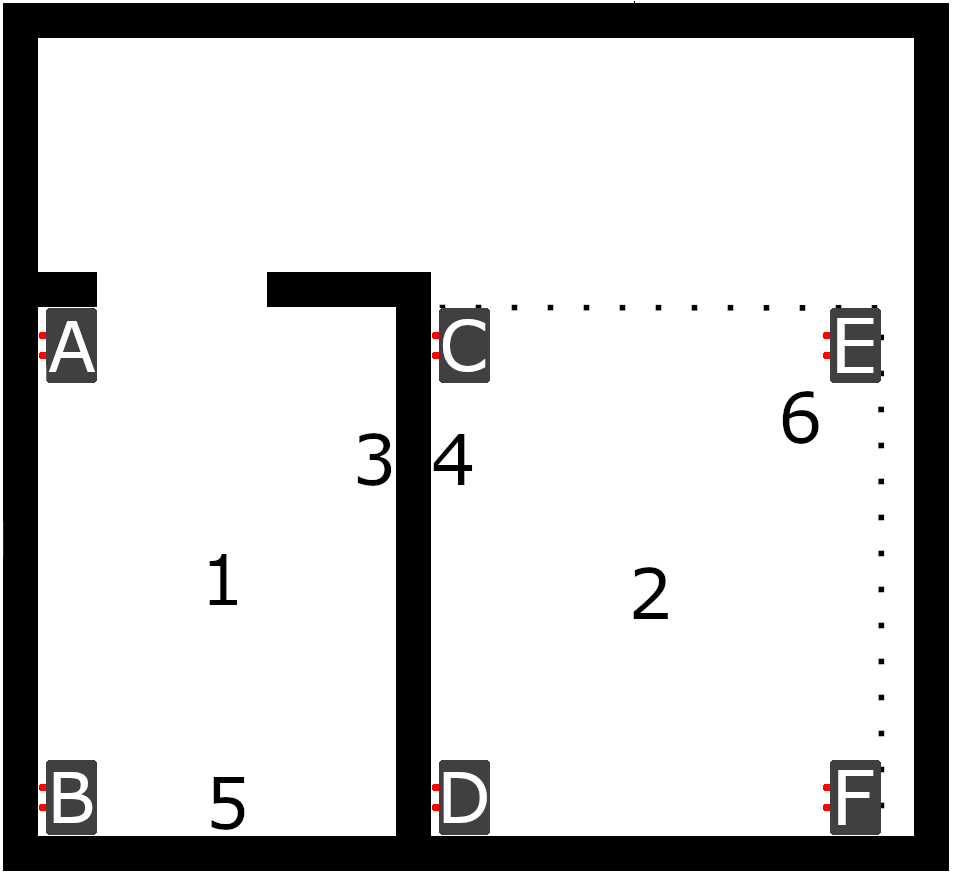
\includegraphics[width=\linewidth]{sble_2_2_floor}
	\captionof{figure}{Meerdere gateways per locatie - Opstelling 2}
	\label{fig:ond-ble-static-2-2-ops}
\end{minipage}

\paragraph{Resultaat}
In deze 2e test is dit scenario er ook weer in geslaagd elke beacon correct te lokaliseren. Hier is wel een extra stap bij de verwerking gekomen. Door het toevoegen van de muur wordt niet elke beacon door elke gateway meer opgevangen. Hierdoor verschijnen er rode platte streepjes in de tabel. Het spreekt voor zich dat dit ook meteen diskwalificerend werkt voor de locatie(s) waarvan deze gateway een hoekpunt is aangezien de beacon niet tussen deze gateways zal liggen als er 1 van deze gateways de beacon niet eens ziet.

\begin{figure}[h]
	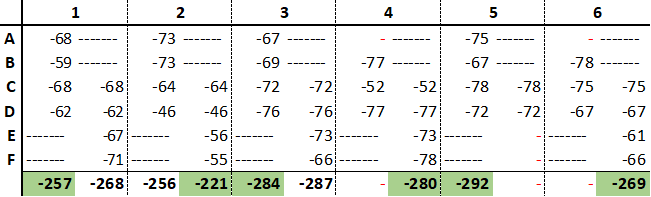
\includegraphics[width=\linewidth]{sble_2_2_results}
	\caption{Meerdere gateways per locatie - Testresultaat 2}
	\label{fig:ond-ble-static-2-2-res}
\end{figure}

\paragraph{Testconclusie}
Op het eerste zicht lijkt deze test volledig geslaagd, het toevoegen van een muur zorgt er niet voor dat dit scenario slechter presteert. Echter is er wel een belangrijk detail dat aangehaald moet worden. Als de cijfers beter onderzocht worden blijkt het volgende: bij elke beacon is de gateway die hem met de hoogste RSSI waarneemt een gateway die in dezelfde ruimte ligt als de beacon. Met andere woorden dezelfde uitkomst kan bekomen worden met 1 gateway per ruimte, en zo wordt de opstelling vereenvoudigd tot het vorige scenario, waarvoor minder gateways nodig zijn.

\subsubsection{Deelconclusie}
Dit scenario blijkt zeer effectief te zijn en heeft alle geteste beacons perfect gelokaliseerd. Echter blijkt wel dat deze opstelling geen voordelen heeft over de vorige (1 gateway / locatie) als een locatie 1 ommuurde ruimte is, maar wel meer hardware vereist. Hiervoor is het dus niet geschikt. Voor lokalisatie in een open ruimte echter, lijkt ze beter te werken, voor een hogere hardware kost. De deelhypothese is bevestigd.

\subsection{Gateways in rasteropstelling}
\subsubsection{Deelhypothese}
Deze opstelling slaagt er in om met een BLE beacon getagde assets een positie te geven binnen het raster zodat het eenduidig met een locatie kan worden gelinkt.

\subsubsection{Test 1: Raster in open, reële ruimte}
\begin{minipage}{0.55\textwidth}
De opstelling voor deze test is idem aan het vorige scenario, test 1. Aangezien bij die test ook beacons in een raster gemeten zijn, kon de data uit die test hier hergebruikt worden en worden verwerkt met trilateratie. Voordat trilateratie kan toegepast worden, moet er eerst een omzetting gebeuren tussen de RSSI waarde en de afstand. Dit kan door de FSPL formule te gebruiken (weliswaar omgekeerd). Aangezien bij de verwerking van de resultaten bleek dat dit niet geheel correct was is nog een offset in dBm toegevoegd, verschillend per soort beacon. Dit om het bij het vooronderzoek vastgelegde fenomeen dat beacons, hoewel ze de zelfde instellingen hebben, niet allen een even sterk signaal sturen. Bij de verwerking is een waarde gebruikt van -16 dB voor de gebruikte H5 beacons, en -10 dB voor de M2 beacons. Deze waardes zijn experimenteel vastgelegd, en vloeien voort uit de data van de afstandstest bij het vooronderzoek, waar de offset van de trendlijn tegenover de theoretische curve is gebruikt.
\end{minipage}
\hfill
\begin{minipage}{0.42\textwidth}
	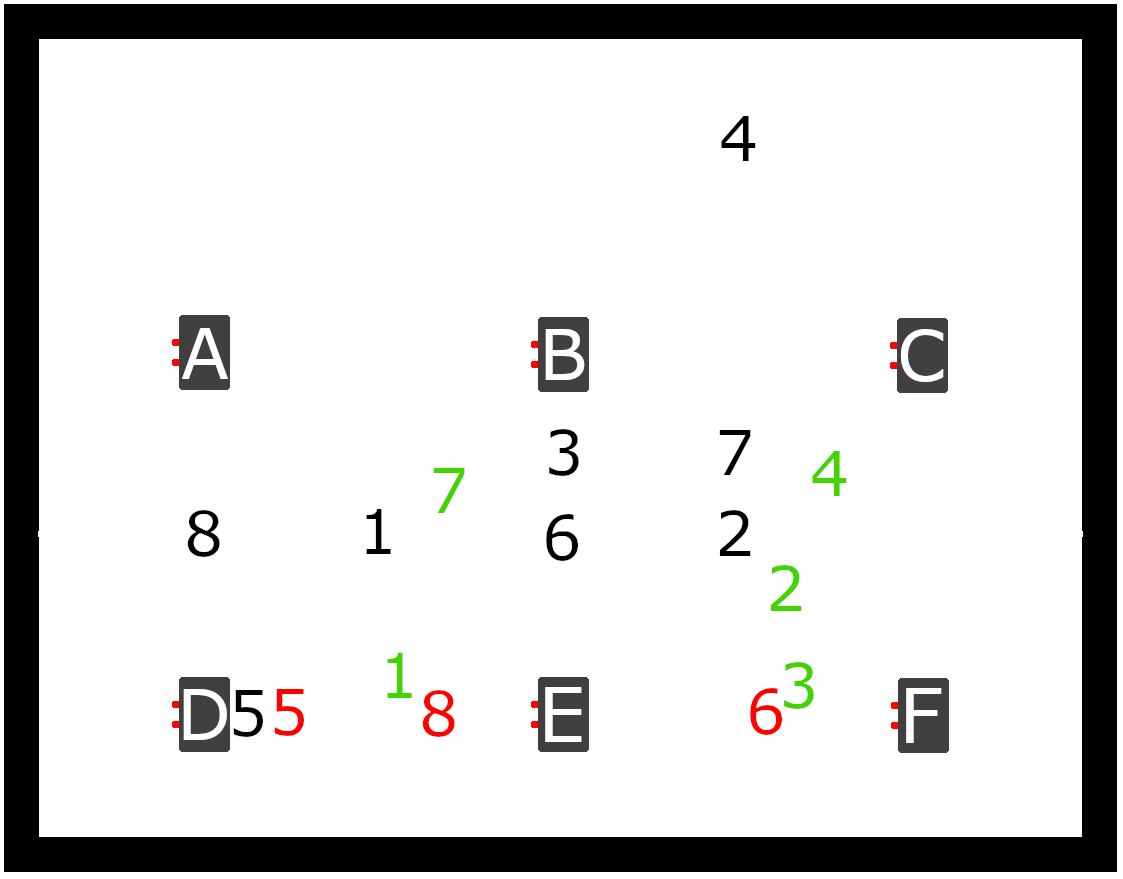
\includegraphics[width=\linewidth]{sble_3_1_floor}
	\captionof{figure}{Gateways in rasteropstelling - Test 1}
	\label{fig:ond-ble-static-3-1}
\end{minipage}

De resultaten van de trilateratie worden geplot op bovenstaand grondplan. De zwarte cijfers zijn de effectieve locaties van de beacons, de gekleurde zijn de berekende locaties a.d.h.v. de resultaten en trilateratie, met de groene een geslaagde trilateratie, en een rode een mislukte. Een mislukte wilt zeggen dat trilateratie niet mogelijk is door te korte afstanden (bv. de afstand tussen beacon 6 en gateway E en F bedraagt resp. 0.87m en 0.62m, dus opgeteld 1.49m. Dit is onmogelijk aangezien de afstand tussen deze beacons 2m bedraagt). Bij een situatie zoals dit is de beacon geplaatst tussen de 2 gateways.

\paragraph{Resultaat}
Om het resultaat te berekenen zijn de 2 gateways met de beste RSSI gebruikt. Meteen is zichtbaar dat het resultaat vrij catastrofaal is en dat de uitkomst van de trilateratie de beacons precies random plaatst. Beacon 5 komt in de buurt, maar deze lag fysiek aan gateway 5, waardoor zijn RSSI zeer hoog was (-28 dBm), hierdoor werd deze door de noodoplossing van het algoritme toch ietwat in de buurt geplaatst maar dit is een unicum. Verder is enkel beacon 2 relatief ok geplaatst.

\paragraph{Testconclusie}
Het is duidelijk dat trilateratie op basis van RSSI zeer onnauwkeurig is. Dit ligt vooral aan het onnauwkeurig omzetten van RSSI waardes in afstanden door de grote onzekerheden op RSSI waardes. Deze eerste test belooft zeker niet veel goeds voor dit concept.

\subsubsection{Test 2: Raster verspreid over gebouw met muren}
\begin{minipage}{0.55\textwidth}
In deze 2e test is het raster vergroot, van 2m maar 3.5m tussen gateways. Ook is het raster verspreid over een gebouw, met muren tussen.
De methodieken voor berekening en de kleurcodes voor het visualiseren van de resultaten zijn gelijk gebleven aan vorige test.
\end{minipage}
\hfill
\begin{minipage}{0.42\textwidth}
	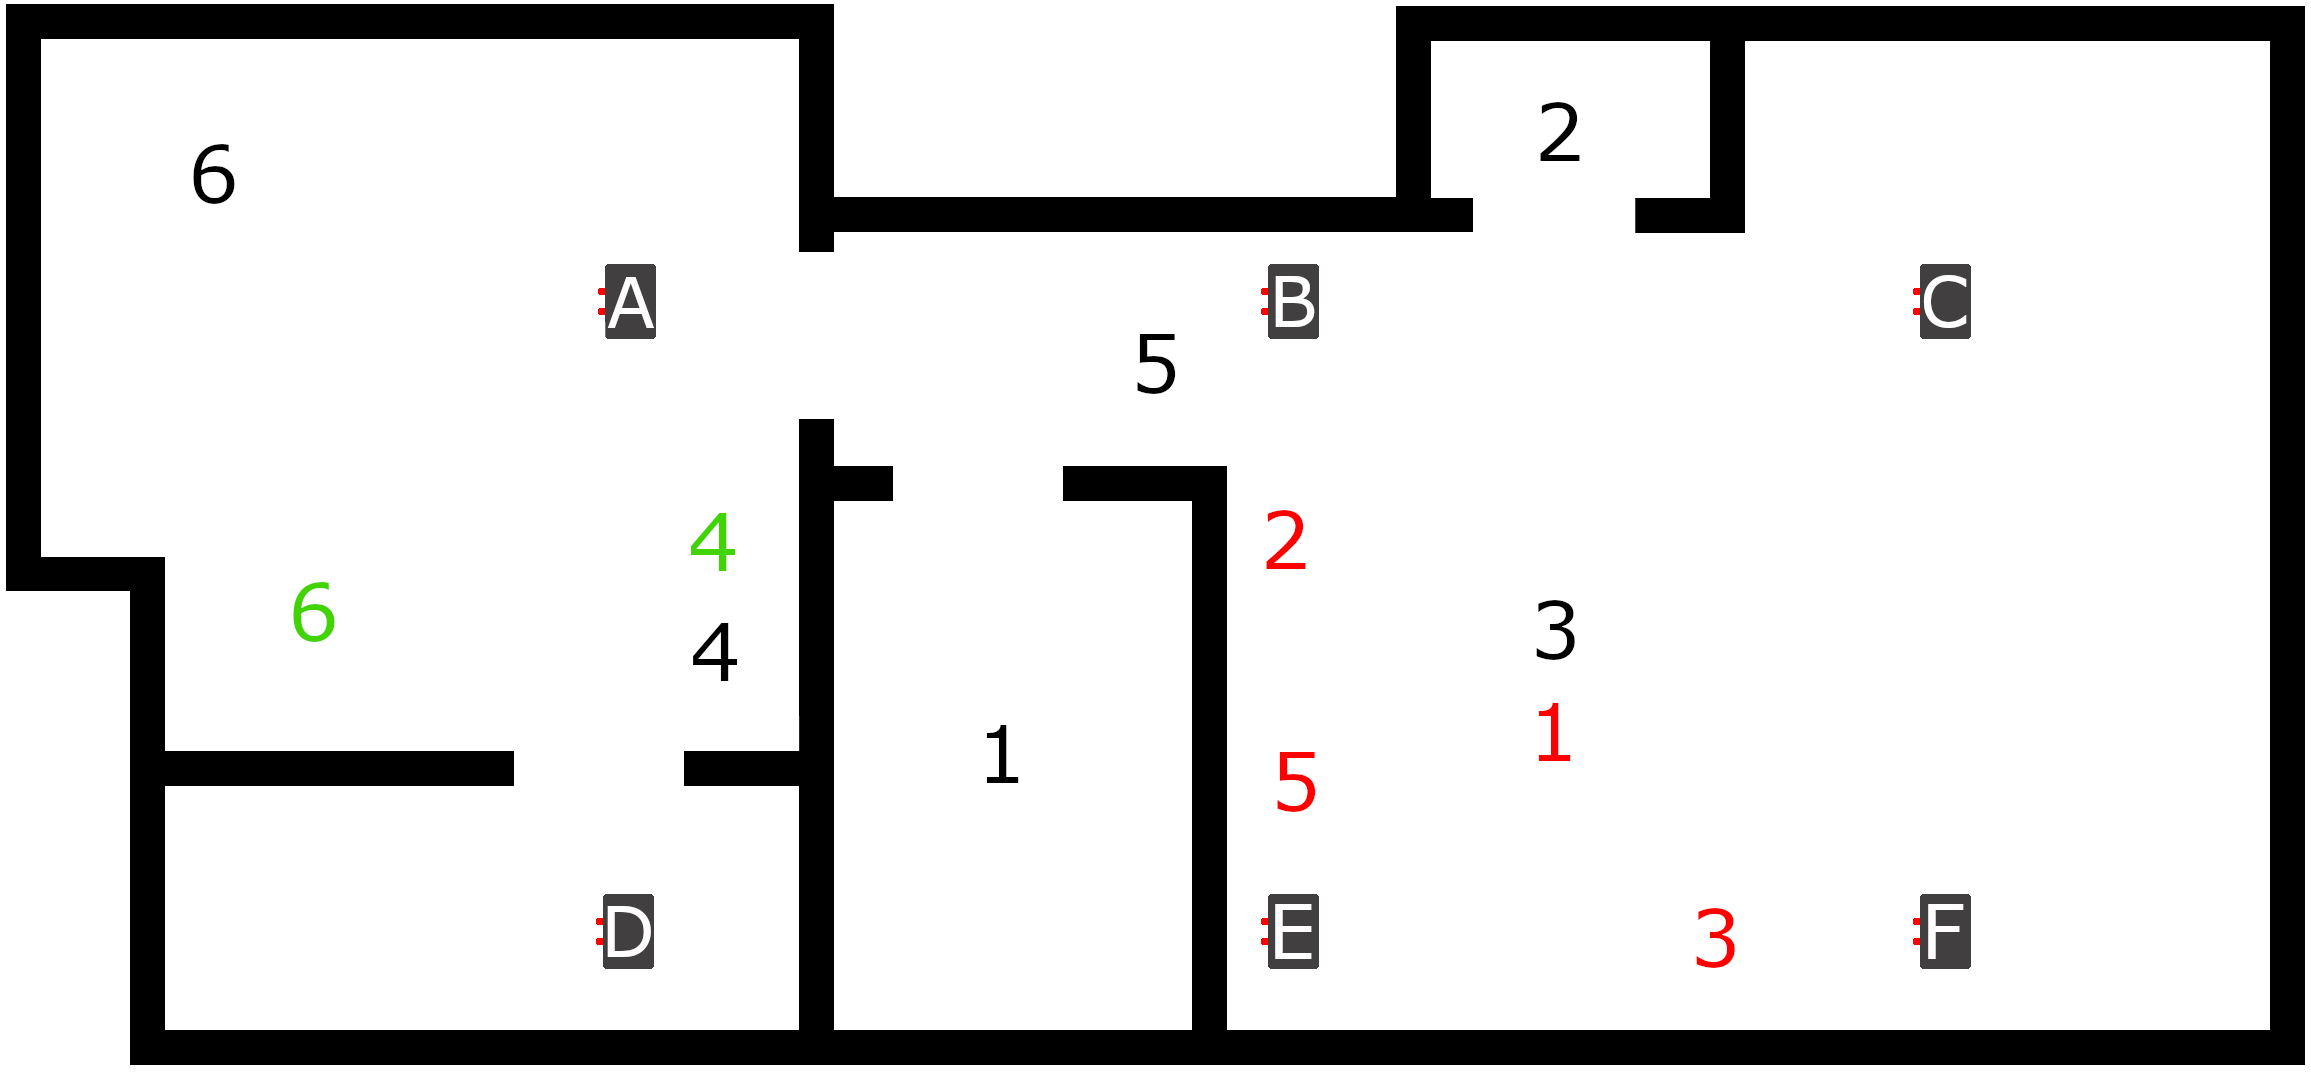
\includegraphics[width=\linewidth]{sble_3_2_floor}
	\captionof{figure}{Gateways in rasteropstelling - Opstelling 2}
	\label{fig:ond-ble-static-3-2-ops}
\end{minipage}

\paragraph{Resultaat}
\begin{minipage}{0.55\textwidth}
Na deze test zijn er slechts 2 beacons die met succes kunnen getrilatereerd worden zonder de noodoplossing te gebruiken (groen). Deze 2 beacons (4 en 6) zijn ook enkel opgemerkt door de 2 gateways waar ze tussen liggen. De 4 andere beacons zijn zeer slecht geplaatst in vergelijking met hun effectieve positie.
\end{minipage}
\hfill
\begin{minipage}{0.42\textwidth}
	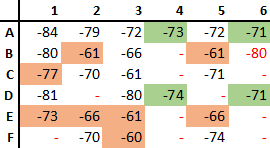
\includegraphics[width=\linewidth]{sble_3_2_results}
	\captionof{figure}{Gateways in rasteropstelling - Testresultaat 2}
	\label{fig:ond-ble-static-3-2-res}
\end{minipage}

\paragraph{Testconclusie}
Deze grotere test heeft weer aangetoond wat na vorige test al duidelijk was, trilateratie op basis van RSSI is onnauwkeurig. En het toevoegen van muren, waardoor niet elke geteway meer elke beacon ziet, heeft de nauwkeurigheid enkel verslecht.

\subsubsection{Deelconclusie}
Na deze 2 tests kan duidelijk worden besloten dat dit scenario niet haalbaar is met de gebruikte BLE hardware. In het principe zit potentieel, maar enkel als er een goeie, precieze conversie kan worden gemaakt tussen RSSI waardes en afstanden. De deelhypothese is hierbij dus ontkracht.

\section{Dynamische BLE}
In tegenstelling tot bij statische BLE opstellingen, is de variabele 'tijd' wel belangrijk bij dynamische BLE opstellingen. Daarom is het essentieel dat de tijd tussen de berichten, ontvangen van de gateway, vrij kort is. Een tussenperiode van 30s is hierbij niet wenselijk, aangezien de gateway zich zeer ver kan verplaatsten op deze tijdsspanne en de metingen dus vrijwel nutteloos zullen zijn. Vandaar dat de instellingen van zowel de beacons als de gateway zullen worden versneld tijdens volgende testen. De gateway zal elke seconde zijn gemeten informatie doorsturen. Verder is het bij deze snelheden niet meer mogelijk om een beacon zendsnelheid van 30 berichten per gatewaybericht aan te houden aangezien de maximale snelheid 10 berichten/seconde bedraagt. Deze maximumsnelheid zal ook worden gebruikt tijdens volgende testen.

\subsection{1 beacon per locatie, midden van locatie}
\subsubsection{Deelhypothese}
Deze opstelling slaagt er in om met een BLE beacon getagde assets correct te lokaliseren.

\subsubsection{Test 1: 3 even grote locaties in open reële ruimte}
\begin{minipage}{0.55\textwidth}
Voor deze test is een open ruimte opgedeeld in een gang en 3 locaties, liggende naast elkaar en langs 1 kant van deze gang. Deze locaties zijn even groot, en voorzien van een locatiebeacon (MokoSmart H5) in hun middelpunt, met een onderlinge afstand van 200cm. Tijdens de test wordt een gateway aan een constante snelheid verplaatst, aangegeven door de pijl op de illustratie. De test duurt 20sec, en op deze tijd heeft de gateway de volledige breedte van de opstelling overbrugd. 
\end{minipage}
\hfill
\begin{minipage}{0.42\textwidth}
	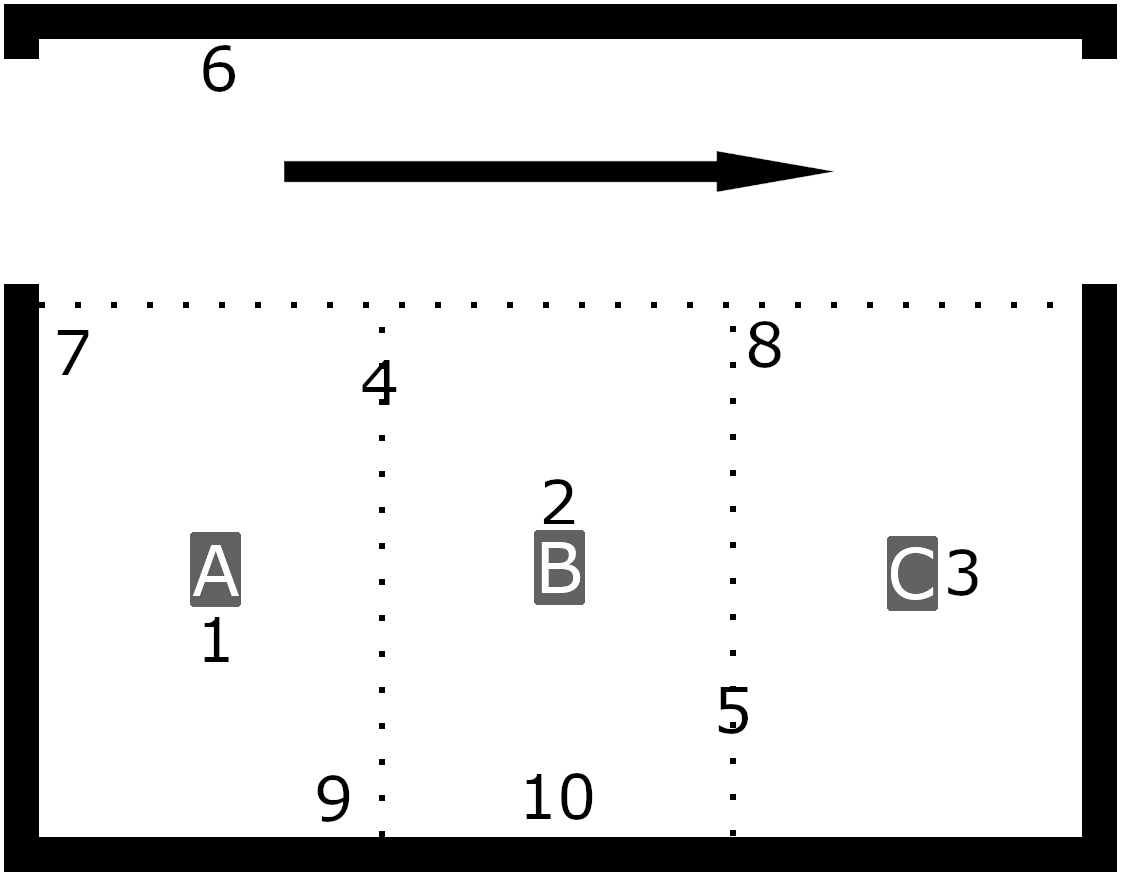
\includegraphics[width=\linewidth]{dble_1_1_floor}
	\captionof{figure}{1 beacon per locatie, midden van locatie - Opstelling 1}
	\label{fig:ond-ble-dynamic-1-1-ops}
\end{minipage}

\paragraph{Resultaat}
\begin{minipage}{0.42\textwidth}
In bijgevoegde tabel zijn de resultaten van deze test zichtbaar. Elke kolom stelt een beacon voor, opgedeeld volgens locatie- en assetbeacons. Voor elke beacon is zijn maximale RSSI waarde aangeduid in groen. Dit punt komt overeen met het moment dat de gateway deze beacon het dichtste nadert en komt dus overeen met het moment dat de gateway de beacon voorbij komt. Hieruit kan afgeleid worden welke beacons in elkaars buurt liggen. 
\end{minipage}
\hfill
\begin{minipage}{0.55\textwidth}
	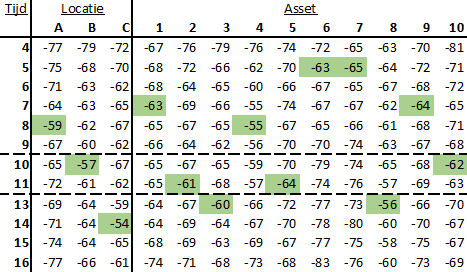
\includegraphics[width=\linewidth]{dble_1_1_results}
	\captionof{figure}{1 beacon per locatie, midden van locatie - Testresultaat 1}
	\label{fig:ond-ble-dynamic-1-1-res}
\end{minipage}

De toewijzing van assetbeacons aan een locatie gebeurt volgens kleinste tijdverschil (een assetbeacon wordt toegewezen aan de locatie waarbij het tijdsverschil tussen zichzelf en de locatiebeacon van die locatie het kleinste is). In bijgevoegde resultatentabel is een onderbroken lijn geplaatst die deze toewijzingen weergeeft.
Vervolgens is uit deze resultaten te concluderen dat deze manier van lokaliseren verrassend goed werkt aangezien elk asset aan de correcte locatie is toegewezen. Beacon 4 en 5 bevinden zich op de grens tussen 2 locaties, en dit is ook zichtbaar aan de resultaten, aangezien hun maximale RSSI dicht bij een overgangslijn valt. Als louter wordt gekeken naar de volgorde zijn er hier en daar enkele onnauwkeurigheden, zoals bv. bij beacons 4 en 9, maar dit verschil is eerder beperkt en verwaarloosbaar als er enkel interesse bestaat voor een locatietoewijzing.

\paragraph{Testconclusie}
Deze eerste test is veelbelovend. Met een zeer eenvoudig lokalisatiealgoritme, gebaseerd op de maximale RSSI waarde, kan een zeer accurate lokalisatie bekomen worden. Wel is het zo dat deze hoogste waardes bij de locatiebeacons vrij dicht bij elkaar liggen, dit vermoedelijk omdat deze beacons dieper in de ruimte liggen en het relatieve afstandsverschil tussen de gateway en de locatiebeacons niet zeer uitgesproken is. Dit zou kunnen vergroot worden door deze beacons dichter naar het gangpad te brengen, of door de gateway nog sneller te laten sturen.

\subsubsection{Test 2: gang omringd door 4 locaties van variabele grootte}
\begin{minipage}{0.55\textwidth}
Deze test maakt gebruik van 4 locaties in verschillende groottes, gescheiden door muren, om zo een realistische gang te bekomen. Verder bevinden deze locaties zich langs beide zijden van de gang. Voor de rest is deze opstelling analoog aan test 1.
\end{minipage}
\hfill
\begin{minipage}{0.42\textwidth}
	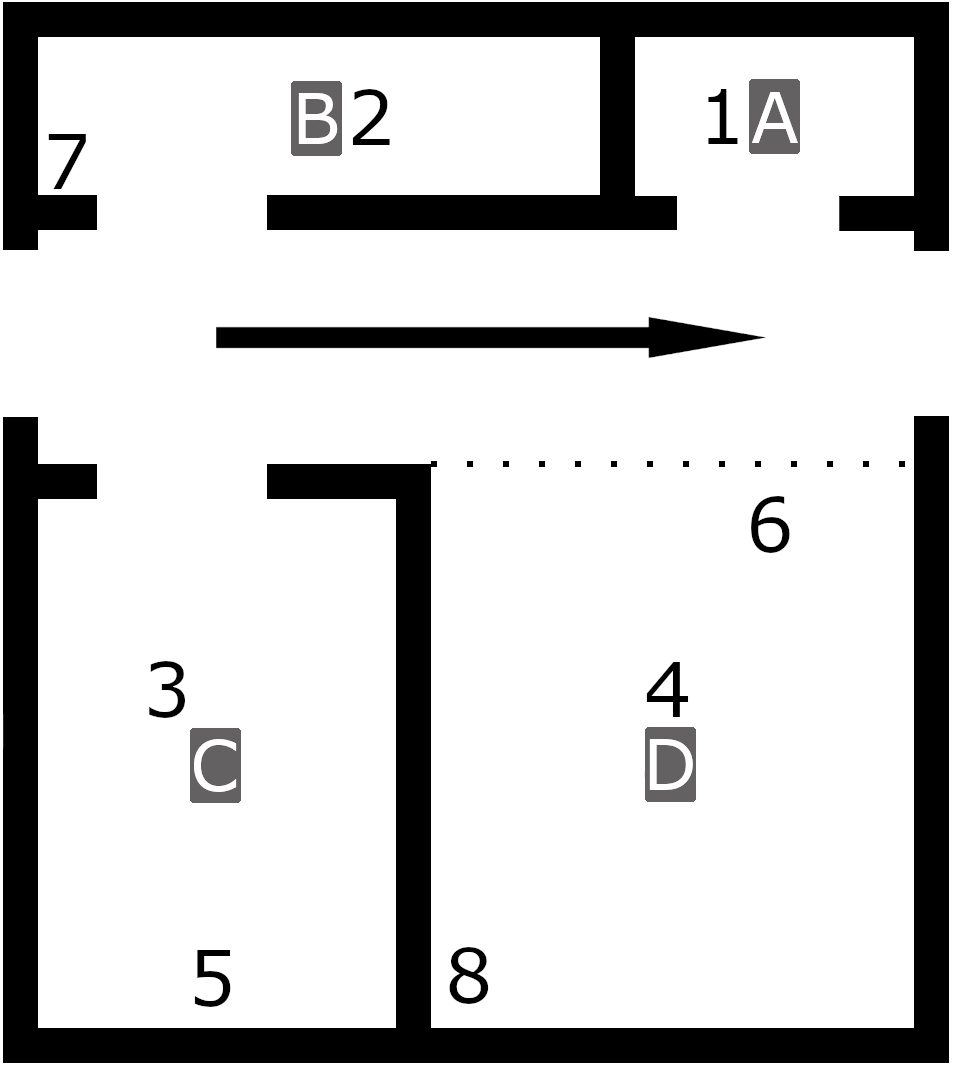
\includegraphics[width=\linewidth]{dble_1_2_floor}
		\captionof{figure}{1 beacon per locatie, midden van locatie - Opstelling 2}
	\label{fig:ond-ble-dynamic-1-2-ops}
\end{minipage}

\paragraph{Resultaat}
\begin{minipage}{0.42\textwidth}
Bijgevoegde tabel toont de resultaten van deze test, volgens dezelfde regels en opbouw als in test 1. Als eerste valt op dat hier slechts 1 scheidingslijn aanwezig is. Dit is bewust. Bij deze test is het zo dat er locaties aanwezig zijn langs beide kanten van de gang, op ongeveer dezelfde hoogte. 
\end{minipage}
\hfill
\begin{minipage}{0.55\textwidth}
	\includegraphics[width=\linewidth]{dble_1_2_results}
	\captionof{figure}{1 beacon per locatie, midden van locatie - Testresultaat 2}
	\label{fig:ond-ble-dynamic-1-2-res}
\end{minipage}

Met 1 MikroTik KNOT gateway is het niet mogelijk richting (links of rechts) te detecteren dus worden deze 2 locaties samengesmolten. Na de vereenvoudiging door deze hardware limitatie blijven er 2 locaties over. De toewijzing van de assets aan deze 2 locaties is echter wel weer perfect gebeurd, en ook de volgorde zit nagenoeg correct.

\paragraph{Testconclusie}
Na deze 2e realistischere test, met toevoeging van muren, is er zichtbaar aan de resultaten dat de lokalisatie even goed (perfect) gebeurt als in de eenvoudigere opstelling van test 1. Wel is het duidelijk dat een links/rechts opdeling handig zou zijn voor een bruikbaarder algoritme, maar dit is enkel hardwarematig op te lossen. Bijvoorbeeld door het gebruik van 2 vlakke antennes, 1 naar rechts en 1 naar links gericht. Dit kan echter gesimuleerd worden door de resultaten op te delen in 2 (1 per richting), en het is duidelijk dat de resultaten in dat geval ook in orde zijn.

\subsubsection{Deelconclusie}
Uit deze testen is af te leiden dat dit principe van opstelling zeer goed werkt, zowel in een open ruimte als met de toevoeging van muren. De deelhypothese is aangenomen.
	

\subsection{1 beacon per locatie, aan deur}
\subsubsection{Deelhypothese}
Deze opstelling slaagt er in om met een BLE beacon getagde assets correct te lokaliseren, en de detectie van de locatiebeacon zal beter zijn dan in het geval dat deze dieper weg zit in de ruimte.

\subsubsection{Test 1: 3 even grote locaties in open ruimte}
\begin{minipage}{0.55\textwidth}
De opstelling voor deze test is analoog aan de opstelling voor het vorige scenario, test 1. Als enige verschil zijn de locatiebeacons verplaatst naar de grens tussen de locaties en de gang.
\end{minipage}
\hfill
\begin{minipage}{0.42\textwidth}
	\includegraphics[width=\linewidth]{dble_2_1_floor}
	\captionof{figure}{1 beacon per locatie, aan deur - Opstelling 1}
	\label{fig:ond-ble-dynamic-2-1-ops}
\end{minipage}

\paragraph{Resultaat}
\begin{minipage}{0.42\textwidth}
De resultaten in bijgevoegde tabel zijn zeer analoog aan deze bij test 1 van het vorige scenario. Met als enige verschil dat de locatiebeacons verder uit elkaar liggen in de tijd. Verder worden alle assets wederom correct gecategoriseerd per locatie, met een onderlinge volgorde van maximale RSSI waardes die ruwweg overeenkomt met de volgorde waarop deze beacons zijn gepasseerd. 
\end{minipage}
\hfill
\begin{minipage}{0.55\textwidth}
	\includegraphics[width=\linewidth]{dble_2_1_results}
	\captionof{figure}{1 beacon per locatie, aan deur - Testresultaat 1}
	\label{fig:ond-ble-dynamic-2-1-res}
\end{minipage}

Als opvallende uitzondering op deze volgorde is er tag 5, welke zeer hard naar voor gesprongen is in de volgorde. Wat nog maar eens onderstreept dat RSSI metingen niet precies zijn, en dat een combinatie van fenomenen zoals reflecties en stralingspatronen toevallige miscategorisaties kunnen veroorzaken. In deze test was dit niet het geval, maar de relatieve plaats van tag 5 is versprongen van op de grens tussen locatie B en C naar de grens tussen locatie A en B.

\paragraph{Testconclusie}
Deze test vertoont, buiten een betere spreiding van de locatiebeacons in de tijd, geen noemenswaardige verschillen met test 1 van het vorige scenario.

\subsubsection{Test 2: gang omringd door 4 locaties van variabele grootte}
\begin{minipage}{0.55\textwidth}
Deze test is analoog aan het vorige scenario, test 2, mat als enige verschil dat de locatiebeacons niet geplaatst zijn in het middelpunt, maar aan de deur.
\end{minipage}
\hfill
\begin{minipage}{0.42\textwidth}
	\includegraphics[width=\linewidth]{dble_2_2_floor}
	\captionof{figure}{1 beacon per locatie, aan deur - Opstelling 2}
	\label{fig:ond-ble-dynamic-2-2-ops}
\end{minipage}

\paragraph{Resultaat}
\begin{minipage}{0.42\textwidth}
Ook bij deze resultaten, zichtbaar in bijgevoegde tabel, zijn de verschillen met de overeenkomstige test uit het vorige scenario ,beperkt. Het enige wat opvalt is dat de maximale RSSI-waardes van locatiebeacons B en C vrij veel zijn verhoogd, wat het gevolg is van de geografie. Locatiebeacon B ligt in dit geval niet meer achter een muur, en C ligt niet meer diep in een kamer, gecombineerd met een muur. 
\end{minipage}
\hfill
\begin{minipage}{0.55\textwidth}
	\includegraphics[width=\linewidth]{dble_2_2_results}
	\captionof{figure}{1 beacon per locatie, aan deur - Testresultaat 2}
	\label{fig:ond-ble-dynamic-2-2-res}
\end{minipage}

\paragraph{Testconclusie}
Het lijkt erop dat het plaatsen van de locatiebeacons aan de deur in een realistische opstelling voordelen heeft tegenover in het midden van de kamer, voornamelijk op vlak van betere RSSI. Dit was niet het geval tijdens test 1 aangezien het effect van muren en deuren afwezig is in deze test. Verder is het wel zo dat een deur (zoals het geval bij beacon B) zich niet noodzakelijk in het midden van de locatie bevind. Dit heeft natuurlijk een affect op de toewijzing, aangezien de overgangslijn/tijd niet meer midden tussen de locatiebeacons moet geplaatst worden, maar verschoven worden afhankelijk van de geografie van de locaties.

\subsubsection{Deelconclusie}
Dit scenario heeft een licht voordeel tegenover vorig scenario, maar enkel als het aankomt op een opstelling niet in een open ruimte. Het lijkt qua detectie en spreiding in de tijd beter om de locatiebeacons dichter bij de gang te hangen. De hypothese is aangenomen.

\subsection{Meerdere locatiebeacons per locatie}
\subsubsection{Deelhypothese}
Deze opstelling slaagt er in om met een BLE beacon getagde assets correct te lokaliseren.

\subsubsection{Test 1: 2 even grote locaties in open ruimte}
\begin{minipage}{0.55\textwidth}
Voor deze test worden er in een open ruimte 2 locaties gecreëerd, met een locatiebeacon (MokoSmart H5) in elke hoek, waarvan bij de 2 overlappende hoeken een gemeenschappelijke locatiebeacon. Deze beacons liggen 2m uit elkaar. Ook zullen er assetbeacons verspreid worden, aangegeven door de cijfers op de figuur. Verder zal een gateway voorbij komen volgens de pijl. 
\end{minipage}
\hfill
\begin{minipage}{0.42\textwidth}
	\includegraphics[width=\linewidth]{dble_3_1_floor}
	\captionof{figure}{Meerdere locatiebeacons per locatie - Opstelling 1}
	\label{fig:ond-ble-dynamic-3-1-ops}
\end{minipage}

\paragraph{Resultaat}
\begin{minipage}{0.42\textwidth}
Na het aggregeren en analyseren van de testdata is zeer snel iets interessants opgevallen, als deze data verwerkt wordt door enkel te kijken naar de locatiebeacons die het dichtst tegen de gang aan liggen, en verder wordt gekeken naar de hoogste RSSI-waardes zoals in de vorige 2 scenario's klopt de lokalisatie perfect mits de grenslijn tegen de locatiebeacon wordt aangelegd. Dit wilt zeggen dat deze opstelling overbodig uitgebreid is en kan herleid worden tot het vorige scenario. 
\end{minipage}
\hfill
\begin{minipage}{0.55\textwidth}
	\includegraphics[width=\linewidth]{dble_3_1_results}
	\captionof{figure}{Meerdere locatiebeacons per locatie - Testresultaat 1}
	\label{fig:ond-ble-dynamic-3-1-res}
\end{minipage}

Interessant is wel dat het ook mogelijk is om hetzelfde resultaat te bekomen met de achterste rij locatiebeacons (aangeduid in licht blauw in bijgevoegde resultatentabel). Het is echter wel duidelijk dat deze punten dichter bij elkaar liggen in de tijd en dus minder nauwkeurig zullen zijn (zoals duidelijk het geval is met assetbeacon 2 en 6, welke in theorie buiten de locatie zouden vallen).

\paragraph{Testconclusie}
Dit scenario is overbodig complex en kan vereenvoudigd worden tot het vorige. Deze test heeft wel nogmaals bevestigd dat het voor de precisie beter is als de locatiebeacons dichter bij de gang liggen.

\subsubsection{Test 2: 2 even grote locaties gescheiden door muur}
\begin{minipage}{0.55\textwidth}
In deze testopstelling is een muur toegevoegd tussen de 2 locaties van de testopstelling van test 1. Verder blijft de opstelling gelijk.
\end{minipage}
\hfill
\begin{minipage}{0.42\textwidth}
	\includegraphics[width=\linewidth]{dble_3_2_floor}
	\captionof{figure}{Meerdere locatiebeacons per locatie - Opstelling 2}
	\label{fig:ond-ble-dynamic-3-2-ops}
\end{minipage}

\paragraph{Resultaat}
\begin{minipage}{0.42\textwidth}
Uit het resultaat van deze test, zichtbaar in bijgevoegde tabel, is hetzelfde al te leiden als uit de resultaten van test 1. De helft van de locatiebeacons blijkt overbodig.
\end{minipage}
\hfill
\begin{minipage}{0.55\textwidth}
	\includegraphics[width=\linewidth]{dble_3_2_results}
	\captionof{figure}{Meerdere locatiebeacons per locatie - Testresultaat 2}
	\label{fig:ond-ble-dynamic-3-2-res}
\end{minipage}

\paragraph{Testconclusie}
De toegevoegde muur heeft klaarblijkelijk geen effect op de resultaten, iets wat wel het geval was bij de statische versie van deze opstelling. Deze opstelling is wederom vereenvoudiggebaar naar die van vorig scenario.

\subsubsection{Deelconclusie}
Na deze testen kan afgeleid worden dat dit scenario te ver gezocht is, en hetzelfde resultaat kan bereikt worden met een een eenvoudigere opstelling en minder hardware. Alhoewel te hypothese technisch gezien correct is, zal dit scenario niet als beste uit de bus komen na dit onderzoek.

\subsection{Beacons in rasteropstelling}
\subsubsection{Deelconclusie}
Na de zeer slechte testresultaten van de statische versie van dit scenario, en omdat dit scenario zich qua principe berust op dubbele trilateratie, waardoor de extreme onnauwkeurigheden bij enkele trilateratie enkel maar extremer zullen worden, is besloten dit scenario niet nader te onderzoeken.

\subsection{Beacons op intervallen in de gang}
\subsubsection{Deelhypothese}
Deze opstelling slaagt er in om met een BLE beacon getagde assets correct te lokaliseren.

\subsubsection{Test 1: 3 even grote locaties in open ruimte}
\begin{minipage}{0.55\textwidth}
De opstelling voor deze test is gelijkaardig aan de opstelling van het 1e dynamische scenario, test 1. Met als verschil dat de locaties niet meer 1 op 1 worden gedefinieerd door een locatiebeacon, maar dat deze locatiebeacons op gelijke afstand verspreid liggen in de gang (specifiek op 250cm onderlinge afstand). In deze opstelling bevinden de locatiegrenzen zich op resp. 2/3 de afstand tussen A en B, en op 1/3 de afstand tussen B en C. De rest van de afmetingen en opstelling zijn identiek.
\end{minipage}
\hfill
\begin{minipage}{0.42\textwidth}
	\includegraphics[width=\linewidth]{dble_4_1_floor}
	\captionof{figure}{Beacons op intervallen in de gang - Opstelling 1}
	\label{fig:ond-ble-dynamic-4-1-ops}
\end{minipage}

\paragraph{Resultaat}
\begin{minipage}{0.42\textwidth}
Ook de voorstelling van de resultaten, zichtbaar in bijgevoegde tabel, is gelijkaardig. De plaatsing van de scheidingslijn tussen de verschillende locaties is echter wel verschillend. Aangezien de locatie van de locatiegrenzen en de beacons niet meer aan elkaar gelinkt zijn, hangt het af van de specifieke opstelling hoe deze zich tot elkaar verhouden. Hier is dit 2/3 en 1/3, en door recht evenredige verhouding tussen de afstand en de tijd door de constante snelheid is de scheidingslijn ook zo geplaatst in de tabel.
\end{minipage}
\hfill
\begin{minipage}{0.55\textwidth}
	\includegraphics[width=\linewidth]{dble_4_1_results}
	\captionof{figure}{Beacons op intervallen in de gang - Testresultaat 1}
	\label{fig:ond-ble-dynamic-4-1-res}
\end{minipage}

Na deze andere manier van locatietoewijzing zien we dat de lokaliseringsresultaten nog steeds goed overeen komen met de werkelijkheid. Dit met uitzondering van beacon 1, welke versprongen is versprongen van de eerste naar de laatste locatie. Dit fenomeen is al eerder tegengekomen in een eerdere test (5.4.2, test 1), en wordt daar besproken.

\paragraph{Testconclusie}
Deze test vertoont analoge resultaten aan eerdere scenario's.

\subsubsection{Test 2: gang omringd door 4 locaties van variabele grootte}
\begin{minipage}{0.55\textwidth}
De opstelling voor deze test is gelijkaardig aan de opstelling van het 1e dynamische scenario, test 2. Idem aan test 1 worden de locatiebeacons geplaatst op gelijke afstanden in de tussenliggende gang. De locatieovergang tijdens deze test is vlak voor locatiebeacon B aan de rechterkant, en 1/3 de afstand tussen B en C langs de linkerkant van de gang.
\end{minipage}
\hfill
\begin{minipage}{0.42\textwidth}
	\includegraphics[width=\linewidth]{dble_4_2_floor}
	\captionof{figure}{Beacons op intervallen in de gang - Opstelling 2}
	\label{fig:ond-ble-dynamic-4-2-ops}
\end{minipage}

\paragraph{Resultaat}
\begin{minipage}{0.42\textwidth}
Bijgevoegde tabel met resultaten is licht anders opgedeeld dan soortgelijke tabellen uit vorige tests, dit omdat er een opdeling is gemaakt tussen rechts en links van de gang. Dit is eenderzijds om een simulatie te maken voor een opstelling die een richting kan bepalen, en anderzijds omdat de definitie voor locatieovergang langs rechts en links verschilt, dus 1 lijn niet correct was geweest.
Er is duidelijk te zien in de resultaten dat de lokalisatie goed is gebeurt en elk asset in de juiste locatie is ingedeeld.
\end{minipage}
\hfill
\begin{minipage}{0.55\textwidth}
	\includegraphics[width=\linewidth]{dble_4_2_results}
	\captionof{figure}{Beacons op intervallen in de gang - Testresultaat 2}
	\label{fig:ond-ble-dynamic-4-2-res}
\end{minipage}

\paragraph{Testconclusie}
Uit deze test is duidelijk dat ook in een reële situatie, assetbeacons in de gang een goede oplossing kan zijn.

\subsubsection{Deelconclusie}
Dit scenario heeft zeer gelijkaardige resultaten aan dynamisch scenario 1 en 2. Het verschil met deze scenario's is echter wel dat bij deze niet elke locatie een beacon nodig heeft, en de hardware kost dus lager is. Ook is het mogelijk de locatiedefinitie te veranderen zonder de hardware te moeten verhangen, wat een voordeel kan geven voor sommige use cases.

%...

%%=============================================================================
%% Conclusie
%%=============================================================================

\chapter{Conclusie}
\label{ch:conclusie}
\section{Informatiebundeling}
\label{sec:con-inf}
Voordat een algemene conclusie getrokken kan worden, is het interessant alle relevante informatie op een rijtje te plaatsen. Hieronder volgt een opsomming van alle onderzochte opstellingen, waarbij voor elk hun toepassingsgebied wordt bijgevoegd, alsook de eventuele \textcolor{ForestGreen}{voor-} en \textcolor{RedOrange}{nadelen}. Al deze informatie is reeds beschikbaar in het corpus en voornamelijk de deelconclusies in hoofdstuk~\ref{ch:testen}. De informatie voor de algemene voor- en nadelen wordt gehaald uit hoofdstuk~\ref{ch:opstellingen}. Deze gelden voor elke opstelling in de specifieke technologie.

Ook wordt er een benadering gegeven voor de kostprijs, de informatie voor deze berekening is reeds beschikbaar in hoofdstuk~\ref{ch:methodologie}. Deze kostprijs \(K\) wordt uitgedrukt als \(K = f(l, a)\) met \(l\) het aantal locaties en \(a\) het aantal assets. Dit zijn de 2 voornaamste schaalfactoren voor de kosten.

Het doel van deze sectie is een gestructureerde weergave van de meest interessante informatie te geven, als basis voor het nemen van de feitelijke eindconclusie.

\subsection{RFID Algemeen}
\label{sec:con-ant-RFID}
\paragraph{Voor- en nadelen}
\begin{itemize}
	\color{ForestGreen}
	\item Goedkope tags
	\item Tags vereisen geen/minimaal onderhoud
	\color{RedOrange}
	\item Dure uitrolkosten
	\item Tags enkel detecteerbaar in RFID doorgang
	\item Tagoriëntatie in de RFID doorgang is belangrijk
\end{itemize}

\subsection{BLE Algemeen}
\label{sec:con-ant-BLE}
\paragraph{Voor- en nadelen}
\begin{itemize}
	\color{ForestGreen}
	\item Beacons steeds detecteerbaar
	\item Goedkope uitrolkosten
	\item Tagoriëntatie verwaarloosbaar
	\color{RedOrange}
	\item Beacons vereisen onderhoud
	\item Relatief dure beacons
	\item Grote variatie op RSSI waarden
\end{itemize}

\subsection{Static RFID: 1 antenne aan deurlijst}
Bruikbaar bij afgesloten ruimtes met (smalle) toegangen als locatie.
\paragraph{Voor- en nadelen}
\begin{itemize}
\color{ForestGreen}
\item Goedkoopste/minimale RFID optie
\color{RedOrange}
\item Geen richtingsdetectie
\item Enkel te gebruiken in deurdoorgang
\end{itemize}
\paragraph{Kostprijs}
\(K = 1400 \cdot l + 0.01 \cdot a\)

\emph{De kostprijs per locatie kan verlaagd worden door meerdere antennes op 1 transceiver aan te sluiten, als de in-/uitgangen van deze locaties dicht genoeg bij elkaar liggen}

\subsection{Static RFID: 2 antennes aan deurlijst}
Bruikbaar bij afgesloten ruimtes met (smalle) toegangen als locatie.
\paragraph{Voor- en nadelen}
\begin{itemize}
	\color{ForestGreen}
	\item Richtingsdetectie
	\color{RedOrange}
	\item Past moeilijker in deurlijst door breedte 2 antennes + eventuele tussenafstand bij bredere doorgang.
	\item Enkel te gebruiken in deurdoorgang
\end{itemize}
\paragraph{Kostprijs}
\(K = 1450 \cdot l + 0.01 \cdot a\)

\emph{De kostprijs per locatie kan verlaagd worden door 2 antenneparen op 1 4-port transceiver aan te sluiten, als de in-/uitgangen van deze locaties dicht genoeg bij elkaar liggen}

\subsection{Static RFID: 1 antenne tegenover deur}
Bruikbaar bij afgesloten ruimtes met een (korte) gang als toegang, als locatie.
\paragraph{Voor- en nadelen}
\begin{itemize}
	\color{ForestGreen}
	\item Richtingsdetectie
	\item Slechts 1 antenne
	\color{RedOrange}
	\item Vereist langere gang dan enkel deurdoorgang voor goede werking
\end{itemize}
\paragraph{Kostprijs}
\(K = 1400 \cdot l + 0.01 \cdot a\)

\emph{De kostprijs per locatie kan verlaagd worden door meerdere antennes op 1 transceiver aan te sluiten, als de in-/uitgangen van deze locaties dicht genoeg bij elkaar liggen}

\subsection{Dynamic RFID: 1 tag aan deurlijst}
Bruikbaar bij afgesloten ruimtes met (smalle) toegangen, als locatie.
\paragraph{Voor- en nadelen}
\begin{itemize}
	\color{ForestGreen}
	\item Goedkoop door slechts 1 reader
	\color{RedOrange}
	\item Niet noodzakelijk detectie van \emph{alle} aanwezige assets.
\end{itemize}
\paragraph{Kostprijs}
\(K = 1400 + 0.01 \cdot (l + a)\)

\subsection{Static BLE: 1 gateway per locatie}
Bruikbaar bij alle reële locaties gescheiden door muren.
\paragraph{Voor- en nadelen}
\begin{itemize}
	\color{ForestGreen}
	\item Goedkoop
	\item Eenvoudig
	\color{RedOrange}
	\item Niet goed bruikbaar bij meerdere locaties in open ruimte.
\end{itemize}
\paragraph{Kostprijs}
\(K = 100 \cdot l + 10 \cdot a\)

\subsection{Static BLE: meerdere gateways per locatie}
Overal bruikbaar, bij reële locaties gescheiden door muren vereenvoudiging mogelijk.
\paragraph{Voor- en nadelen}
\begin{itemize}
	\color{ForestGreen}
	\item Goede werking bij meerdere locaties in open ruimte.
	\color{RedOrange}
	\item Hogere hardwarekost
	\item Kan worden vereenvoudigd
\end{itemize}
\paragraph{Kostprijs}
\(K = 400 \cdot l + 10 \cdot a\)

\emph{Veronderstelling van omringing door 4 gateways, meer of minder is mogelijk.}

\subsection{Static BLE: gateways in rasteropstelling}
Nergens bruikbaar
\paragraph{Voor- en nadelen}
\begin{itemize}
	\color{ForestGreen}
	\item Lagere hardwarekost door geen 1:1 relatie tussen locatiebeacons en locaties
	\item Locatiedefinities veranderbaar zonder hardware aanpassingen
	\color{RedOrange}
	\item Werkt niet
	\item Meer overhead door nood aan locatiedefiniëring
\end{itemize}
\paragraph{Kostprijs}
\(K = \ll100 \cdot l + 10 \cdot a\)

\emph{Er kan ook meer dan 1 gateway per locatie in een raster staan, in dat geval zijn er echter goedkopere opstellingen mogelijk}

\subsection{Dynamic BLE: 1 locatiebeacon per locatie, midden van locatie}
Overal bruikbaar
\paragraph{Voor- en nadelen}
\begin{itemize}
	\color{ForestGreen}
	\item Lage hardwarekost
	\item Werkt overal
	\color{RedOrange}
	\item Geen real-time detectie
	\item Hoog batterijgebruik
\end{itemize}
\paragraph{Kostprijs}
\(K = 100 + 10 \cdot (l + a)\)

\subsection{Dynamic BLE: 1 locatiebeacon per locatie, aan deur}
Overal bruikbaar
\paragraph{Voor- en nadelen}
\begin{itemize}
	\color{ForestGreen}
	\item Lage hardwarekost
	\item Werkt overal
	\item Nauwkeurigere detectie dan met beacon in midden van kamer
	\color{RedOrange}
	\item Geen real-time detectie
	\item Meer overhead als deur met beacon niet in midden van kamer zit
	\item Hoog batterijgebruik
\end{itemize}
\paragraph{Kostprijs}
\(K = 100 + 10 \cdot (l + a)\)

\subsection{Dynamic BLE: meerdere locatiebeacons per locatie}
Overal bruikbaar, bij reële locaties gescheiden door muren vereenvoudiging mogelijk.
\paragraph{Voor- en nadelen}
\begin{itemize}
	\color{ForestGreen}
	\item Lage hardwarekost
	\item Werkt overal
	\color{RedOrange}
	\item Geen real-time detectie
	\item Kan worden vereenvoudigd
	\item Hoog batterijgebruik
\end{itemize}
\paragraph{Kostprijs}
\(K = 100 + 10 \cdot (l + a)\)

\subsection{Dynamic BLE: locatiebeacons in rasteropstelling}
Nergens bruikbaar
\paragraph{Voor- en nadelen}
\begin{itemize}
	\color{ForestGreen}
	\item Nog lagere hardwarekost door geen 1:1 relatie tussen locatiebeacons en locaties
	\item Locatiedefinities veranderbaar zonder hardware aanpassingen
	\color{RedOrange}
	\item Werkt niet
	\item Meer overhead door nood aan locatiedefiniëring
	\item Hoog batterijgebruik
\end{itemize}
\paragraph{Kostprijs}
\(K = 100 + 10 \cdot (\ll l + a)\)

\emph{Er kan ook meer dan 1 locatiebeacon per locatie in een raster staan, in dat geval zijn er echter goedkopere opstellingen mogelijk}

\subsection{Dynamic BLE: locatiebeacons op intervallen in de gang}
Overal bruikbaar
\paragraph{Voor- en nadelen}
\begin{itemize}
	\color{ForestGreen}
	\item Nog lagere hardwarekost door geen 1:1 relatie tussen locatiebeacons en locaties
	\item Locatiedefinities veranderbaar zonder hardware aanpassingen
	\color{RedOrange}
	\item Geen real-time detectie
	\item Meer overhead door nood aan locatiedefiniëring
	\item Hoog batterijgebruik
\end{itemize}
\paragraph{Kostprijs}
\(K = 100 + 10 \cdot (\ll l + a)\)

\emph{Er kan ook meer dan 1 locatiebeacon per locatie in de gangen hangen, in dat geval zijn er echter goedkopere opstellingen mogelijk}

\section{Een antwoord op de onderzoeksvraag}
\label{sec:con-ant}
Na opsomming van de belangrijkste conclusies van alle onderzochte opstellingen in sectie~\ref{sec:con-inf}, is de tijd gekomen om een antwoord te formuleren op de onderzoeksvraag van dit onderzoek. Deze vraag luid als volgt \footnote{Zie Sectie~\ref{sec:onderzoeksvraag} op pagina~\pageref{sec:onderzoeksvraag}}.:
\begin{center}
	\textbf{Welke hardwareopstelling, bestaande uit RFID of BLE componenten, is optimaal voor de plaats- en verplaatsingsbepaling van een voorwerp binnen een gebouw.}
\end{center}

Om een antwoord te geven op deze onderzoeksvraag moet een vergelijking gemaakt worden tussen alle opstellingen. Een goed begin hiervoor is bij de gebruikte technologie.

\paragraph{RFID vs BLE}
Zoals aangehaald in secties~\ref{sec:con-ant-RFID} en~\ref{sec:con-ant-BLE} heeft elk van deze technologieën zijn voor- en nadelen. Echter is hier de vraag welke van deze voor- en nadelen het meeste doorweegt voor een goede en bruikbare lokalisatieopstelling. 
Het fundamentele voordeel van BLE op dit vlak is nog steeds dat de getagde assets steeds zichtbaar zijn voor het systeem, en er altijd zeker is geweten of het asset aanwezig is, en waar, dit is niet het geval bij RFID. 

Verder heeft BLE een voordeel door de lagere uitrolkosten van een systeem, wat de aanschafdrempel voor heel wat bedrijven, zeker deze met een kleiner budget, kan verlagen. De opschalingskosten, met name deze om meer assets te taggen, zijn hoger dan bij RFID, maar dit is voor toepassingen met een beperkt aantal assets niet zo'n probleem. Ook kan dit geleidelijk aan gebeuren samen met de groei van een bedrijf. Bijvoorbeeld een initiële investering van €5000 voor een systeem en elk jaar €2000 voor nieuwe beacons is realistisch, maar een uitrolkost van €50000 voor een RFID systeem, hoe klein de kost daarna ook mag zijn is veel onaantrekkelijker. Slechts als de kosten van de beacons in de buurt komt van de initiële kost van een RFID opstelling kan er een degelijke vergelijking gemaakt worden. Deze argumenten in acht nemend is het duidelijk dat BLE met oog op de onderzoeksvraag voor dit onderzoek de bovenhand heeft. De beste opstelling zal hierdoor komen uit de 8 BLE opstellingen.

\paragraph{Statisch vs Dynamisch}
Het volgende bestaande onderscheid is deze tussen de statische en dynamische opstellingen. Hier is het zo dat bij beide categorieën opstellingen bestaan die een perfecte lokalisatie bekomen van de assets. Hier bestaat een gelijkstand. Echter is dit niet het enige criteria in de onderzoeksvraag. Ook de detectie van een verplaatsing is vereist, en op dit vlak is er een falen van de dynamische opstellingen. Dit voornamelijk door hun fundamentele niet real-time aard. Bij dynamische opstellingen worden de assets enkel gedetecteerd als de gateway rondgaat in het gebouw. Op dat moment kan een asset al lang verplaatst zijn en is deze niet, of in het beste geval later gedetecteerd. In tegenstelling tot een statische opstelling, waarbij deze verplaatsing meteen wordt gedetecteerd van zodra de gemeten RSSI waarden zo veranderen dat deze bij een andere locatie wordt gecategoriseerd. Statische opstellingen hebben een betere, of op zijn minst snellere detectie, van een verplaatsing. 

Verder is het wel zo dat de kostprijs van een statische opstelling hoger licht dan deze van een dynamische. Echter is dit verschil niet zo uitgesproken, en nog steeds draagbaar (€100 voor een gateway is niet zo veel, en zeker niet zo veel meer dan de €10 voor een beacon). Verder is er qua kostprijs ook de onderhoudskost te bekijken. Voor een dynamische opstelling moeten de beacons op elk moment zeer snel staan ingesteld, wat de batterijduur veel verkort en waardoor er sneller nieuwe batterijen, of nieuwe beacons als de batterij onvervangbaar is, nodig zijn. Bij statische opstellingen kunnen de beacons veel trager ingesteld staan en nog steeds een acceptabele lokalisatie geven, met langere batterijduur tot gevolg. Daarom zal de beste opstelling een van de drie statische opstellingen zijn.

\paragraph{De keuze}
Na vorige schiftingen blijven er nog 3 opstellingen over. Als eerste is het duidelijk dat de rasteropstelling niet de beste is, aangezien deze zeer slechte resultaten leverde. Verder is het, qua toepassingsgebied, duidelijk dat de opstelling met meerdere gateways per locatie de beste is uit de 2 overgebleven, aangezien deze werkt in een open ruimte en de opstelling met 1 gateway niet. Echter is het zo dat bij een situatie waarbij elke locatie omringt is door een muur, deze kan vereenvoudigd worden naar de opstelling met 1 gateway per locatie. Een combinatie van deze 2 opstellingen lijkt hierdoor het meest toegewezen om het probleem aangekaart in de onderzoeksvraag op te lossen.

\paragraph{Het effectieve antwoord}
Het antwoord op de onderzoeksvraag luid als volgt:
\begin{center}
	\textbf{Een combinatie van 2 statische BLE opstellingen, nl. 1 gateway per locatie voor ommuurde locaties, en meerdere gateways per locatie voor meerdere locaties in een open ruimte, is optimaal voor de plaats- en verplaatsingsbepaling van een voorwerp binnen een gebouw.}
\end{center}

\section{Nawoord}
Het is ook duidelijk dat, hoewel dit de beste optie is als antwoord op de onderzoeksvraag zoals ze gesteld is, het merendeel van de andere opstellingen ook hun toepassingsgebied hebben. 

Statische RFID opstellingen, hoewel hier achterwege gelaten voornamelijk door de hoge initiële kost, heeft toepassingen bij zeer hoge volumes assets. Dit is ook niet verrassend aangezien toepassingen van deze opstellingen de voornaamste bezigheid is van Aucxis, en zeker voor de toevoeging van BLE aan hun palmares. 

Dynamische BLE opstellingen hebben ook uitermate goed gepresteerd, en hier zit zeker potentieel in. Het leent zich meer voor concepten zoals inventarisatie, waarbij de eis kan zijn dat er 1x per dag een update van locaties moet zijn en de mobiele gateway bv. aan de kar van de poetsvrouw kan hangen. Echter is het niet geschikt voor (real-time) verplaatsingsdetectie zoals de eis was voor dit onderzoek.

\section{Verder onderzoek}
Dit onderzoek is voornamelijk bedoeld als verkennend, het verkennen van veel verschillende soorten opstellingen zonder al te diep erop in te gaan. Er is nu een antwoord uit de bus gekomen, maar dit is in essentie de optie die het meeste kans maakt om optimaal te zijn. Hierbij is verder onderzoek nodig naar de invloed van verschillende factoren die tijdens dit onderzoek constant zijn genomen. Dit zijn voornamelijk de invloed van de grootte van de locaties (opschalen van de testopstelling) en de invloed van de zendsterkte van de beacons. Maar verder ook meer specifieke variabelen zoals de soort gateway en beacons, de inhoud van de locaties (qua meubels en eventueel reflecterende materialen), het soort muren en deuren en zo veel andere beïnvloedende factoren. Het spreekt voor zich dat een onderzoek naar al deze factoren een onderzoek is van dezelfde grootteorde als deze, en dit niet meer bij de scope van dit onderzoek hoort.

Verder zijn tijdens dit onderzoek de opstellingen in een raster met trilateratie gefaald door de limitatie van het zeer onjuiste omrekening van RSSI waardes naar afstand. Echter is dit niet de enige mogelijkheid om uit deze data een locatie te bepalen, en hoogstwaarschijnlijk kan er, na enig onderzoek, een algoritme bedacht worden die wel acceptabele resultaten geeft. Dit lag echter ook buiten de scope van dit onderzoek.

%%=============================================================================
%% Bijlagen
%%=============================================================================

\appendix
\renewcommand{\chaptername}{Appendix}

%%---------- Onderzoeksvoorstel -----------------------------------------------

\chapter{Onderzoeksvoorstel}
Het onderwerp van deze bachelorproef is gebaseerd op een onderzoeksvoorstel dat vooraf werd beoordeeld door de promotor. Dat voorstel is opgenomen in deze bijlage.
\section{Introductie} % The \section*{} command stops section numbering
\label{sec:introductie}

Dit onderzoek zal draaien rond het onderzoeken en vergelijken van verschillende tracking technologieën, zowel actieve als passieve, in verschillende use-cases. Dit zal worden gedaan in samenwerking met Auxcis. Dit bedrijf wilt hun bestaande aanbod Track and Trace oplossingen, welke momenteel berusten op het gebruik van passieve RFID tags, uitbreiden met oplossingen gebaseerd op actieve technologieën (zoals BLE, CenTrak, UHF, GPS enz.). Voordat ze dit willen verwezelijken zijn zij geïnteresseerd in een onderzoek naar de voor- en nadelen, en toepassingsgebieden/use-cases van de verschillende actieve technologieën die realistisch door hun inzetbaar zijn.

Tegenwoordig wordt er steeds meer gebruik gemaakt van trackingtechnologiëen, echter is het in vele gevallen moeilijk te kiezen tussen de technologie waarvan gebruik zal gemaakt worden aangezien de specificaties verschillen tussen deze technologiëen. Het doel van dit onderzoek is dan ook het kiezen tussen deze verschillende opties gemakkelijker maken, door op een overzichtelijke manier deze verschillende opties met hun voor-en nadelen, en toepassingsgebieden weer te geven.

Practisch gezien zullen deze verschillende toepassingsgebieden vooral onderscheden worden door het bereik (samenhangend met de grootte van het gebouw) en de nauwkeurigheid/detectiegraad (samenhangend met de grootte van het voorwerp, en de snelheid van verplaatsing) van de technologie, alsook het verschil tussen een statische en dynamische setup. Ook andere factoren zoals kost (Hardware, licence fees et.), het effect van meerdere verdiepingen en gemak van integratie in bestaande systemen zullen van belang zijn, en deze zullen dus ook opgenomen worden in het onderzoek en conclusies.

%---------- Stand van zaken ---------------------------------------------------

\section{State-of-the-art}
\label{sec:state-of-the-art}

\subsection{Actieve vs. passieve trackingtechnologieën}

Actieve trackers versturen voortdurend een signaal welke opgevangen kan worden door een basisstation, en zo kan in real-time de positie van de tracker (en bij uitbreiding het voorwerp of de persoon waaraan deze verbonden is) gelocaliseerd en gevolgd worden.
Dit in tegenstelling tot pasieve trackers, welke een locatie opslaan, die later kan uitgelezen worden om de locatiegeschiedenis te bepalen. \autocite{Rosenfeld2017}

\subsection{Waarom dit onderzoek?}
De keuze tussen de verschillende technologieën is niet gemakkelijk en zeer afhankelijk van de toepassing. Echter zijn er niet veel tot geen bronnen vindbaar die deze vergelijking maken. De bronnen die er zijn focussen zich voornamelijk op de voornaamste speler, GPS, gevolgd door satteliettracking en gebruik van het mobiel netwerk. Alhoewel dit zeer bruikbare technologieën zijn zijn deze niet geschikt voor de toepassing in gebouwen, aangezien zij niet nauwkeurig genoeg zijn, en problemen hebben bij de aanwezigheid van verdiepingen. Andere meer besproken technologieën zijn BLE en WiFi, welke veelbelovend zijn, maar er bestaan geen vergelijkingen met andere minder bekende technologieën zoals CenTrak. Dit onderzoek is bedoeld ondersteuning te bieden bij deze keuze. \autocite{Deloitte2021} \autocite{Nijhawan2021}

%---------- Methodologie ------------------------------------------------------
\section{Methodologie}
\label{sec:methodologie}

Het onderzoek zal voornamelijk experimenteel verlopen, met testopstellingen van de fysieke hardware (opgesteld op het kantoor van Auxcis). De kwantitatieve resultaten (nauwkeurigheid, detectiegraad, bereik enz.) zullen hiermee worden bepaald. Voor het bepalen van het gemak van integratie in bestaande infrastructuur zal een server gebouwd worden met Dotnet, welke zal dienen als 'vertaler' tussen de fysieke infrastructuur en de bestaande servers van Auxcis. Alhoewel de resultaten op dit vlak voornamelijk een mening van mezelf zullen zijn (moeilijkheidsgraad is subjectief), zijn hier ook meetbare parameters zoals aantal werkuren en aantal lijnen code aan verbonden. Dus ook hier zijn kwantitatieve conclusies uit te trekken. Factor kost zal uiteraard vooral afhangen van de betaalde prijs van de opstelling, uiteraard gestandaardiseerd om alle technologieën hetzelfde te beoordelen.

%---------- Verwachte resultaten ----------------------------------------------
\section{Verwachte resultaten}
\label{sec:verwachte_resultaten}

Aangezien het doel van dit onderzoek een vergelijking maken is, zullen de resultaten grotendeels kunnen worden neergeschreven in een tabel, met een rij voor elke technologie en een kolom voor elke gemeten/bepaalde variabele. Ook zal aan elke technologie een score worden gegeven op basis van de geschiktheid voor een bepaalde toepassing, met hiervoor ook een boomdiagram voor het maken van een keuze van technologie.

%---------- Verwachte conclusies ----------------------------------------------
\section{Verwachte conclusies}
\label{sec:verwachte_conclusies}

Ik verwacht dat een klassieke technologie zoals GPS het slecht zal doen tegenover meer moderne en kleinschaligere technologieën met basisstations zoals BLE of CenTrak, door de slechtere nauwkeurigheid. Welke van de andere technologieën op welke vlakken zal uitschijnen zal afhangen van het onderzoek. Alhoewel ik denk dat CenTrak het goed zal doen aangezien dit voornamelijk is ontworpen voor de tracking van objecten binnen een ziekenhuis dus dit heeft zijn toepassing al mee.

%%---------- Andere bijlagen --------------------------------------------------
%\input{...}

%%---------- Referentielijst --------------------------------------------------
%\chapter{Bibliografie}
\printbibliography[heading=bibintoc]
\end{document}
